\documentclass{cmspaper}
\usepackage{graphicx}
\usepackage{amsmath}
\usepackage{amssymb}
\usepackage{subfigure}
\usepackage{multirow}
\usepackage[pdfborder=0 0 0,
            colorlinks,
            urlcolor = blue,
            linkcolor = black,
            citecolor = black,
            menucolor = black,]
           {hyperref}
%% \usepackage[colorlinks]{hyperref}
%% \usepackage{url}
\usepackage[toc,page]{appendix}
\renewcommand{\appendixname}{Appendix}
%% \renewcommand{\appendixtocname}{List of appendices}

% % useful definitions

% processes
\def\dyee {\ensuremath{Z/\gamma^*\to ee}}
\def\dymm {\ensuremath{Z/\gamma^*\to\mu\mu}}
\def\dytt {\ensuremath{Z/\gamma^*\to\tau\tau}}
\def\zee {\ensuremath{Z\to ee}}
\def\zmm {\ensuremath{Z\to\mu\mu}}
\def\ztt {\ensuremath{Z\to\tau\tau}}
\def\ttbar {\ensuremath{t\bar{t}}}
\def\wwll {\ensuremath{WW\to l^+l^-}}
\def\wwlulu{\ensuremath{WW\to l^+\nu l^-\bar{\nu}}}
\def\ww {\ensuremath{WW}}
\def\hww {\ensuremath{H\to WW}}
\def\wz{\ensuremath{WZ}}
\def\zz{\ensuremath{ZZ}}
\def\wgamma{\ensuremath{W\gamma}}
\def\wjets{\ensuremath{W+}jets} 
\def\tw{\ensuremath{tW}} 
\def\singletopt{\ensuremath{t} ($t$-chan)} 
\def\singletops{\ensuremath{t} ($s$-chan)} 
\def\all{all}
\def\ee{\ensuremath{ee}}
\def\emu{\ensuremath{e\mu}}
\def\mm{\ensuremath{\mu\mu}}

%units
\newcommand{\TeV}{\ensuremath{\mathrm{Te\kern -0.1em V}}}
\newcommand{\GeV}{\ensuremath{\mathrm{Ge\kern -0.1em V}}}

%others
\def\pt{\ensuremath{p_T}}
\def\ipb{pb\ensuremath{^{-1}}}
\def\ifb{fb\ensuremath{^{-1}}}
\def\et{\ensuremath{E_T}}
\def\met{\ensuremath{E\!\!\!\!/_T}}
\def\fBrem{\ensuremath{f_{\rm brem}}}
\def\pin{\ensuremath{p_{\rm in}}}
\def\pout{\ensuremath{p_{\rm out}}}

\newcommand{\CLs}{\ensuremath{CL_\mathrm{s}}}
\newcommand{\CLb}{\ensuremath{CL_\mathrm{b}}}
\newcommand{\CLsb}{\ensuremath{CL_\mathrm{s+b}}}

\newcommand{\GeV}{\ensuremath{\mathrm{Ge\kern -0.1em V}}}
\newcommand{\TeV}{\ensuremath{\mathrm{Te\kern -0.1em V}}}
\newcommand{\TeVcc}{\ensuremath{\,\mathrm{Te\kern -0.1em V\!/c}^2}}
\newcommand{\GeVcc}{\ensuremath{\,\mathrm{Ge\kern -0.1em V\!/c}^2}}
\newcommand{\MeVcc}{\ensuremath{\,\mathrm{Me\kern -0.1em V\!/c}^2}}
\newcommand{\GeVc}{\ensuremath{\mathrm{Ge\kern -0.1em V}\!/c}}
\newcommand{\nanob}{\mbox{{\rm ~nb}~}}
\newcommand{\fb}{\ensuremath{\mathrm{fb}}}
\newcommand{\pb}{\ensuremath{\mathrm{pb}}}
\newcommand{\ifb}{\ensuremath{\mathrm{fb^{-1}}}}
\newcommand{\ipb}{\ensuremath{\mathrm{pb^{-1}}}}
\newcommand{\grad}{\ensuremath{^{\circ}}}
%
% Special user made math symbols
%
\newcommand{\lsim}{\raisebox{-1.5mm}{$\:\stackrel{\textstyle{<}}{\textstyle{\sim}}\:$}}
\newcommand{\gsim}{\raisebox{-1.5mm}{$\:\stackrel{\textstyle{>}}{\textstyle{\sim}}\:$}}

% particles

\newcommand{\pipm}{\ensuremath{\pi^{\pm}}}
\newcommand{\pizero}{\ensuremath{\pi^{0}}}
\newcommand{\Hi}{\ensuremath{\mathrm{H}}}
\newcommand{\W}{\ensuremath{\mathrm{W}}}
\newcommand{\Wjets}{\ensuremath{\mathrm{W+jets}}}
\newcommand{\Zjets}{\ensuremath{\mathrm{Z+jets}}}
\newcommand{\Wt}{\ensuremath{\mathrm{Wt}}}
\newcommand{\Wstar}{\ensuremath{\mathrm{W}^{*}}}
\newcommand{\Wparenthesisstar}{\ensuremath{\mathrm{W}^{(*)}}}
\newcommand{\WW}{\ensuremath{\W^+\W^-}}
\newcommand{\Z}{\ensuremath{\mathrm{Z}}}
\newcommand{\Zstar}{\ensuremath{\mathrm{Z}^{*}}}
\newcommand{\Astar}{\ensuremath{\mathrm{\gamma}^{*}}}
\newcommand{\ZZ}{\ensuremath{\Z\Z}}
\newcommand{\WZ}{\ensuremath{\W\Z}}
\newcommand{\Wgstar}{\ensuremath{\W\Astar}}
\newcommand{\E}{\ensuremath{\mathrm{e}}}
\newcommand{\Ep}{\ensuremath{\mathrm{e}^{+}}}
\newcommand{\Em}{\ensuremath{\mathrm{e}^{-}}}
\newcommand{\Epm}{\ensuremath{\mathrm{e}^{\pm}}}
\newcommand{\Emp}{\ensuremath{\mathrm{e}^{\mp}}}
\newcommand{\M}{\ensuremath{\mu}}
\newcommand{\Mp}{\ensuremath{\mu^{+}}}
\newcommand{\Mm}{\ensuremath{\mu^{-}}}
\newcommand{\Mpm}{\ensuremath{\mu^{\pm}}}
\newcommand{\Mmp}{\ensuremath{\mu^{\mp}}}
\newcommand{\Tau}{\ensuremath{\tau}}
\newcommand{\Nu}{\ensuremath{\nu}}
\newcommand{\Nubar}{\ensuremath{\bar{\nu}}}
\newcommand{\Lep}{\ensuremath{\ell}}
\newcommand{\Lepp}{\ensuremath{\ell^{+}}}
\newcommand{\Lepm}{\ensuremath{\ell^{-}}}
\newcommand{\Lprime}{\ensuremath{\Lep^{\prime}}}
\newcommand{\Prot}{\ensuremath{\mathrm{p}}}
\newcommand{\Pbar}{\ensuremath{\bar{\mathrm{p}}}}
\newcommand{\PP}{\Prot\Prot}
\newcommand{\PPbar}{\Prot\Pbar}
\newcommand{\ttbar}{\ensuremath{\mathrm{t}\bar{\mathrm{t}}}}
\newcommand{\qq}{\ensuremath{\mathrm{q}\mathrm{q}}}
%\newcommand{\bbbar}{\ensuremath{\mathrm{b}\bar{\mathrm{b}}}}
\newcommand{\Wtb}{\ensuremath{\W\mathrm{t}\mathrm{b}}}
\newcommand{\Top}{\ensuremath{\mathrm{t}}}
\newcommand{\Bot}{\ensuremath{\mathrm{b}}}
\newcommand{\Atop}{\ensuremath{\bar{\mathrm{t}}}}
\newcommand{\Abot}{\ensuremath{\bar{\mathrm{b}}}}
% arrow
\newcommand{\To}{\ensuremath{\rightarrow}}

% masses
\newcommand{\mHi}{\ensuremath{m_{\mathrm{H}}}}
\newcommand{\mW}{\ensuremath{m_{\mathrm{W}}}}
\newcommand{\mZ}{\ensuremath{m_{\mathrm{Z}}}}
\newcommand{\mll}{\ensuremath{m_{\Lep\Lep}}}
\newcommand{\mt}{\ensuremath{m_{\mathrm{T}}}}

% kinematics
\newcommand{\pt}{\ensuremath{p_\mathrm{T}}}
\newcommand{\ptveto}{\ensuremath{\pt^\mathrm{veto}}}
\newcommand{\ptl}{\ensuremath{p_\perp^{\Lep}}}
\newcommand{\ptlmax}{\ensuremath{p_{\mathrm{T}}^{\Lep,\mathrm{max}}}}
\newcommand{\ptlmin}{\ensuremath{p_{\mathrm{T}}^{\Lep,\mathrm{min}}}}
\newcommand{\met}{\ensuremath{\Et^{\mathrm{miss}}}}
\newcommand{\delphill}{\ensuremath{\Delta\phi_{\Lep\Lep}}}
\newcommand{\deletall}{\ensuremath{\Delta\eta_{\Lep\Lep}}}
\newcommand{\delphimetl}{\ensuremath{\Delta\phi_{\met\Lep}}}
\newcommand{\Et}{\ensuremath{E_\mathrm{T}}}
\newcommand{\delR}{\ensuremath{\Delta R}}
\newcommand{\Eta}{\ensuremath{\eta}}

%efficiencies
\newcommand{\effsig}{\ensuremath{\varepsilon_{\mathrm{bkg}}^{\mathrm{S}}}}
\newcommand{\effnorm}{\ensuremath{\varepsilon_{\mathrm{bkg}}^{\mathrm{N}}}}
\newcommand{\Nsig}{\ensuremath{N_{\mathrm{bkg}}^{\mathrm{S}}}}
\newcommand{\Nnorm}{\ensuremath{N_{\mathrm{bkg}}^{\mathrm{N}}}}

% processes
\newcommand{\dyee}{\ensuremath{Z/\gamma^*\to ee}}
\newcommand{\dymm}{\ensuremath{Z/\gamma^*\to\mu\mu}}
\newcommand{\dytt}{\ensuremath{Z/\gamma^*\to\tau\tau}}
\newcommand{\dyll}{\ensuremath{Z/\gamma^*\to\ell\ell}}
\newcommand{\dy}{\ensuremath{Z/\gamma^*}}
\newcommand{\zee}{\ensuremath{Z\to ee}}
\newcommand{\zmm}{\ensuremath{Z\to\mu\mu}}
\newcommand{\ztt}{\ensuremath{Z\to\tau\tau}}
%\newcommand{\ttbar}{\ensuremath{t\bar{t}}}
\newcommand{\ppww}{\ensuremath{pp \to W^+W^-}}
\newcommand{\wwll}{\ensuremath{WW\to \ell^+\ell^-}}
\newcommand{\wwlnln}{\ensuremath{W^+W^-\to \ell^+\nu \ell^-\bar{\nu}}}
\newcommand{\ww}{\ensuremath{WW}}
\newcommand{\wwpm}{\ensuremath{W^+W^-}}
\newcommand{\hww}{\ensuremath{H\to W^+W^-}}
\newcommand{\wz}{\ensuremath{WZ}}
\newcommand{\zz}{\ensuremath{ZZ}}
\newcommand{\wgamma}{\ensuremath{W\gamma}}
\newcommand{\wjets}{\ensuremath{W+}jets} 
\newcommand{\tw}{\ensuremath{tW}} 
\newcommand{\singletopt}{\ensuremath{t} ($t$-chan)} 
\newcommand{\singletops}{\ensuremath{t} ($s$-chan)} 
\newcommand{\zx}{\ensuremath{\mathrm{DY/WZ/ZZ}}}
\newcommand{\zv}{\ensuremath{\mathrm{WZ/ZZ}}}
\newcommand{\z}{\ensuremath{\mathrm{Z}}}
\newcommand{\routin}{\ensuremath{R_{out/in}}}

%other 
\def\fixme{({\bf FixMe})}
\newcommand{\ee}{\ensuremath{ee}}
\newcommand{\emu}{\ensuremath{e\mu}}
\def\mm{\ensuremath{\mu\mu}}

% integrated luminosity
\newcommand{\intlumiSevenTeV}{4.92~\ifb}
\newcommand{\intlumiEightTeV}{1.62~\ifb}

%%%%%%%%%%%
%
\newcounter{myfootertablecounter}

\newcommand\myfootnotemark{%
  %\refstepcounter{footnote}%
  \addtocounter{footnote}{1}%
  \footnotemark[\thefootnote]%
}%

\newcommand\myfootnotetext[1]{%
  \addtocounter{myfootertablecounter}{1}
  \footnotetext[\value{myfootertablecounter}]{#1}
}

% from now on, myfootnote has to be used rather than footnote to
% adapt the myfootercounter
\newcommand\myfootnote[1]{%
  \addtocounter{myfootertablecounter}{1}
  \footnote{#1}
}%



\setcounter{topnumber}{1}
\setcounter{bottomnumber}{1}

%===================================================================================================
\begin{document}
\begin{titlepage}

  \analysisnote{2011/XXX}

  \date{\today}

  \title{Electron Identification Using Multivariate Methods }

  \begin{Authlist}
%
A.~Apyan~\Aref{ 2 },
W.~Andrews~\Aref{ 4 }, 
D.~Barge~\Aref{ 3 }, 
L.~Bauerdick~\Aref{ 1 }, 
G.~Bauer~\Aref{ 2 },
J.~Bendavid~\Aref{ 2 },
K.~Burkett~\Aref{ 1 }, 
E.~Butz~\Aref{ 2 },
C.~Campagnari~\Aref{ 3 }, 
G.~Cerati~\Aref{ 4 },
M.~Chan~\Aref{ 2 },
V.~Dutta~\Aref{ 2 },
D.~Evans~\Aref{ 4 }, 
I.~Fisk~\Aref{ 1 }, 
G.~G\'omez-Ceballos~\Aref{ 2 },
Y.~Gao~\Aref{ 1 }, 
F.~Golf~\Aref{ 4 }, 
M.~Goncharov~\Aref{ 2 },
O.~Gutsche~\Aref{ 1 }, 
K.~Hahn~\Aref{ 2 },
P.~Harris~\Aref{ 6 },
B.~Hooberman~\Aref{ 1 },
S.~Jindariani~\Aref{ 1 },
M.~Klute~\Aref{ 2 },
D.~Kovalskyi~\Aref{ 3 }~\Aref{ 6 }, 
I.~Kravchenko~\Aref{ 5 },
V.~Krutelyov~\Aref{ 3 }, 
A.~Levin~\Aref{ 2 }, 
I.~MacNeill~\Aref{ 4 },
S.~Nahn~\Aref{ 2 },
S.~Padhi~\Aref{ 4 }, 
C.~Paus~\Aref{ 2 },
D.~Ralph~\Aref{ 2 },
F.~Stoeckli~\Aref{ 2 },
K.~Sumorok~\Aref{ 2 },
K.~Sung~\Aref{ 2 },
S.~Tkaczyk~\Aref{ 1 },
Y.~Tu~\Aref{ 4 }, 
F.~W\"urthwein~\Aref{ 4 }, 
R.~Wolf~\Aref{ 2 },
S.~Xie~\Aref{ 2 },
A.~Yagil~\Aref{ 4 }, 
M.~Yang~\Aref{ 2 },
J.~Yoo~\Aref{ 4 },
M.~Zanetti~\Aref{ 2 }
%
\end{Authlist}
\Anotfoot{ 1 }{Fermilab National Accelerator Laboratory, Batavia, USA}
\Anotfoot{ 2 }{Laboratory for Nuclear Science, Massachusetts Institute of Technology, Cambridge, USA}
\Anotfoot{ 3 }{University of California, Santa Barbara, Santa Barbara, USA}
\Anotfoot{ 4 }{University of California, San Diego, San Diego, USA}
\Anotfoot{ 5 }{University of Nebraska-Lincoln, USA}
\Anotfoot{ 6 }{CERN, Switzerland}


  \begin{abstract}
    In this note we implement and study the performance of various multivariate approaches to 
electron identification. A comparison of the performance is made using the Higgs to WW analysis 
as a benchmark. We find overall improvement of $40-50\%$ over the simple cut based electron 
selections used in the past. 
  \end{abstract} 

\end{titlepage}
\tableofcontents
%\listoftables
%\listoffigures
\newpage 

%===================================================================================================
\section{Introduction}
  \label{sec:introduction}
With more than 1\ifb of integrated luminosity we have a sufficiently large \zee\ control sample to obtain a comprehensive understanding of the response of the detector to the presence of real electrons. Through the use of the electron fake rate triggers described in detail in reference \cite{hww_eps}, we also obtain a large enough sample of background electrons from jets to have a good understanding of their behavior. It is natural to try to make use of this new knowledge to gain additional discrimination between signal and background. We make use of standard methods from the TMVA toolkit \cite{tmva} in order to improve discrimination between signal and background electrons. 

To establish a baseline result for performance comparison, we begin with an MVA which uses the following observables, also used in the simple cut based electron selection that has been used in CMS in the past \cite{hww_eps,VBTFCrossSectionNote,ElectronID} :

\begin{itemize}
    \item $\sigma_{i\eta i\eta}$,
    \item $\Delta \eta_{\mathrm{in}}$, 
    \item $\Delta \phi_{\mathrm{in}}$,
    \item $f_{\mathrm{brem}}$ (the fraction of the total momentum carried away by bremstrahlung),
    \item $\sigma_{i\phi i\phi}$,
    \item Number of additional clusters from bremstrahlung,
    \item $1/E_{\mathrm{supercluster}} - 1/p_{\mathrm{GSF\ Track}}$.
\end{itemize}

In this note, the performance is always compared with the cut based electron selection used in the \hww\ analysis for the Lepton Photon 2011 results \cite{hww_lp}.

\section{Data Samples and MVA Training}
\label{sec:training}
There are known differences in a number of important discriminating variables between data and simulation. To ensure that performance of the MVA discriminators is not compromised, we use signal and background electrons from data for the training. In order to avoid complications from trigger inefficiencies, we apply the following set of loose selections on electron candidates that are intended to mimic the high level trigger requirements but applied on offline electron quantities before training:

\begin{itemize}
  \item $\sigma_{i\eta i\eta} < 0.01/0.03$ (barrel/endcap),
  \item $|\Delta\phi_{in}| < 0.15/0.10$,
  \item $|\Delta\eta_{in}| < 0.007/0.009$,
  \item $H/E< 0.12/0.10$,
  \item vertexing conversion rejection,
  \item $|d_{0}| < 0.02$~cm,
  \item $\frac{\sum_{\rm trk}\Et}{\pt^{\rm ele}}<0.2$,
  \item $\frac{\sum_{\rm ECAL}\Et}{\pt^{\rm ele}}<0.2$,
  \item $\frac{\sum_{\rm HCAL}\Et}{\pt^{\rm ele}}<0.2$,
\end{itemize}

These pre-selection cuts are identical to the cuts that define the loose (denominator / fakeable object) electrons used to estimate the fake electron background in the \hww\ analysis\cite{hww_eps}. 

On top of this denominator selection, we apply a loose isolation cut, requiring that the particle flow isolation for electrons defined in the \hww\ analysis is less than $0.20$.  The intention is to factorize the electron identification requirements from the isolation requirements, accounting for correlations by imposing an appropriate isolation cut at the pre-selection level.

Due to qualitative differences in different pseudorapidity regions of the detector, mainly due to differences in the material distribution, we perform the training in three different bins of $\eta$: $|\eta| < 1.0$, $1.0 \le |\eta| < 1.5$, and $1.5 \le |\eta| < 2.5$. Due to dependencies of the electron observables on \pt\ we also divide the training sample into two bins of \pt: $10\ \GeV\ \le \pt < 20\GeV $, and $\pt > 20 \GeV $. Thus, the training of the MVA is performed in a total of 6 bins.

Since data events are used to train the MVA, one must be careful to explicitly split the dataset into training and test samples. We use electrons only from even numbered event numbers for training. Tests of performance and measurements of efficiencies and fake rates are performed only on electrons from odd numbered event numbers. This is an important detail in order to avoid measurement biases.

\subsection{Signal Electron Training Sample}
The signal electron sample is obtained from the DoubleElectron primary dataset, requiring a logical OR of the signal double electron trigger and the tag-and-probe triggers given below:

\begin{itemize}
  \item HLT\_Ele17\_CaloIdL\_CaloIsoVL\_Ele8\_CaloIdL\_CaloIsoVL,
  \item HLT\_Ele17\_CaloIdT\_TrkIdVL\_CaloIsoVL\_TrkIsoVL\_Ele8\_CaloIdT\_TrkIdVL\_CaloIsoVL\_TrkIsoVL,
  \item HLT\_Ele32\_CaloIdL\_CaloIsoVL\_SC17,
  \item HLT\_Ele17\_CaloIdVT\_CaloIsoVT\_TrkIdT\_TrkIsoVT\_SC8\_Mass30.
\end{itemize}

We select events with two electrons passing the denominator selection and isolation requirement given above, and require that the dielectron mass is between $75$ \GeV\ and $105$ \GeV. These requirements reduce the residual background to a negligible level. The mass requirement as well as the trigger selection biases the \pt\ spectrum of such electrons significantly toward the typical \pt\ spectrum for leptons from the decay of a \Z\ boson. In order to arrive at an MVA discriminator that is reasonably optimal for the \hww\ analysis, we reweight this \pt\ spectrum to the spectrum obtained from the \hww\ Monte Carlo simulation with a mass hypothesis of $115$ \GeV. The unweighted and weighted spectra are shown in Figure \ref{fig:SignalPtSpectrum}. 

\begin{figure}[!htbp]
\begin{center}
\subfigure[Unweighted]{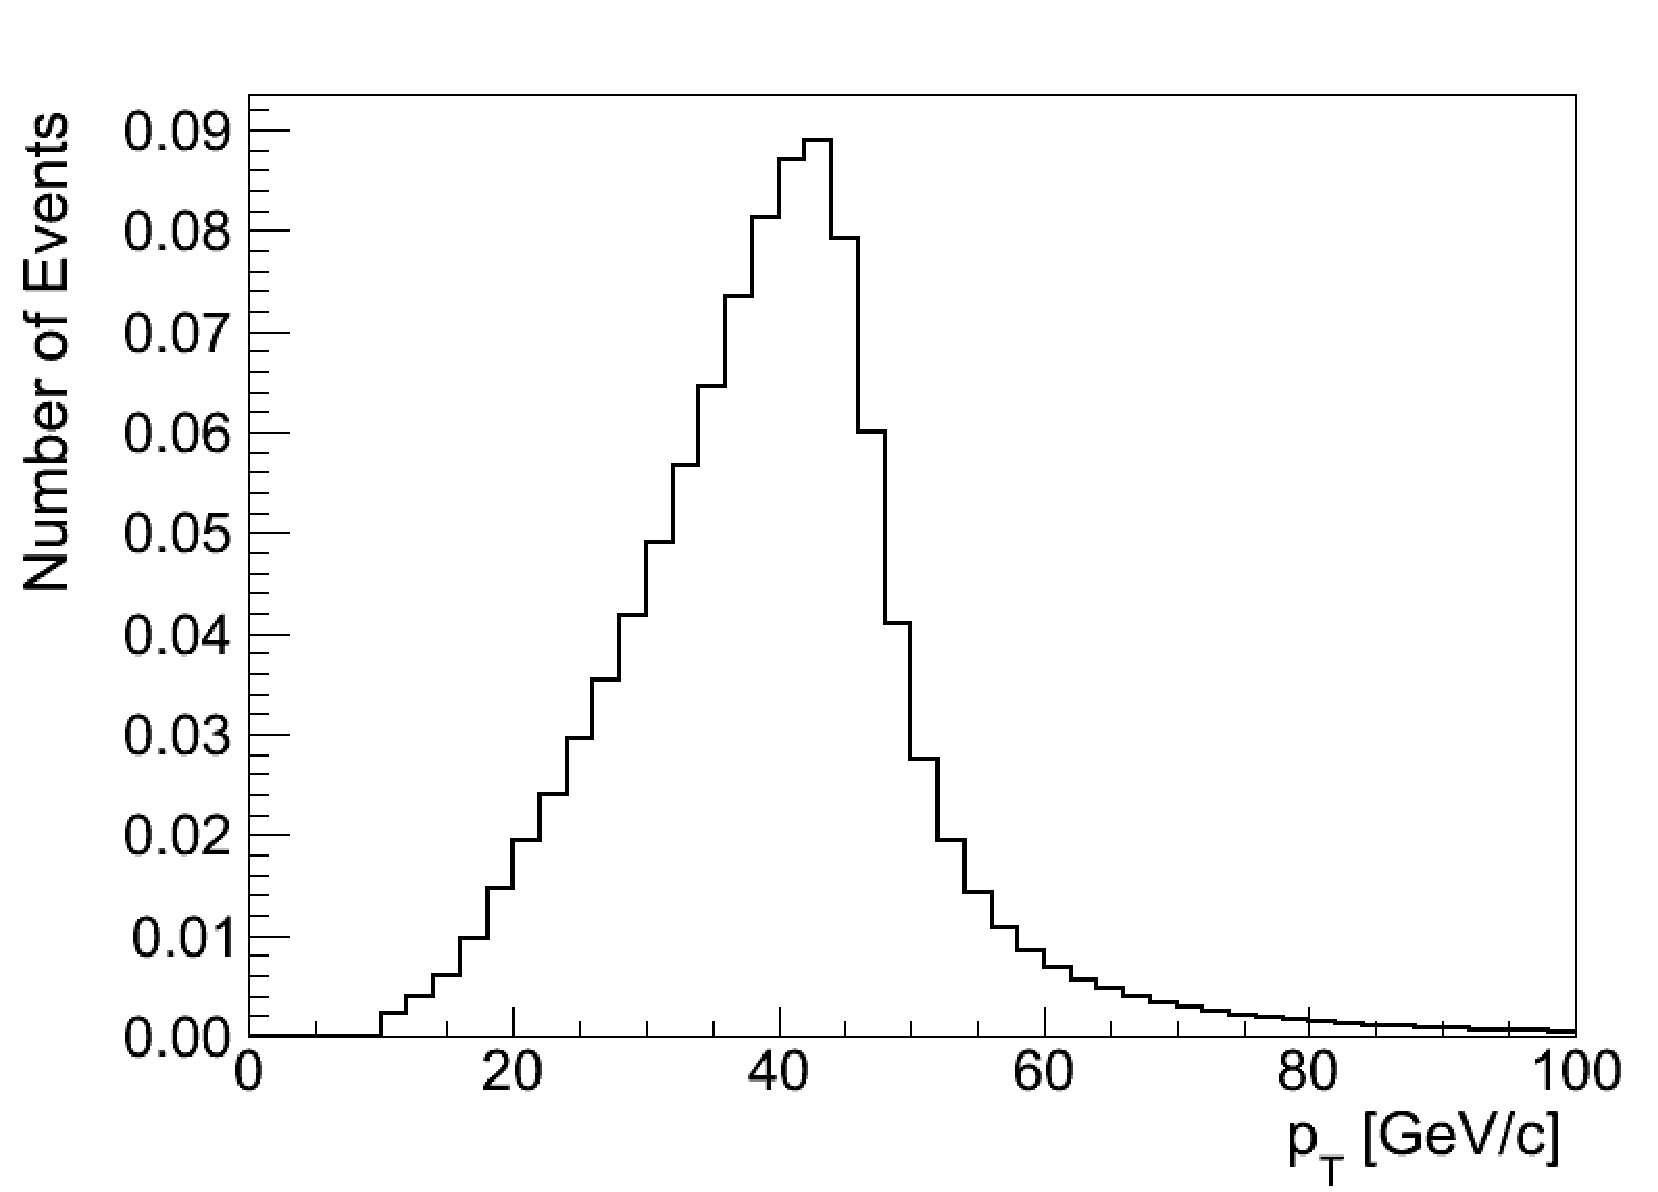
\includegraphics[width=0.45\textwidth]{figures/SignalPt_Source.pdf}}
\subfigure[Weighted]{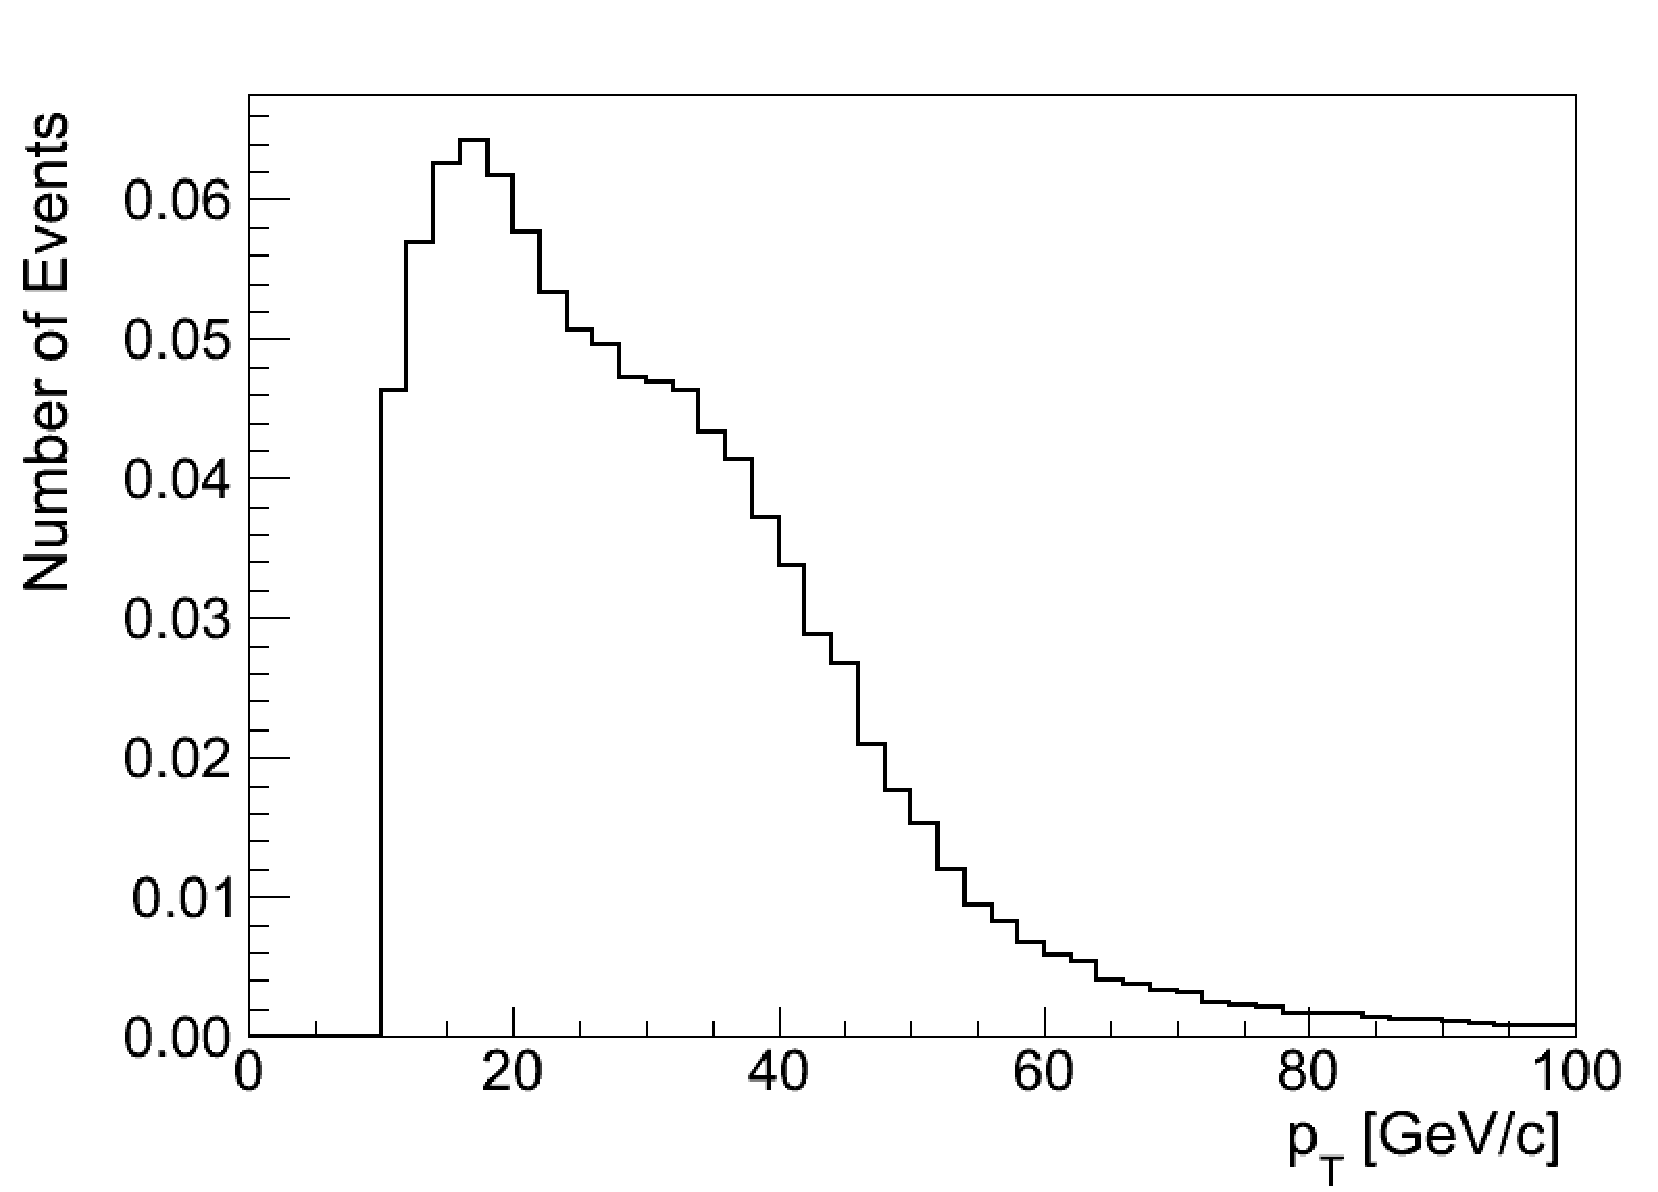
\includegraphics[width=0.45\textwidth]{figures/SignalPt_Target.pdf}}
\caption{The unweighted and weight \pt\ spectrum of the signal electron training sample.}
\label{fig:SignalPtSpectrum}
\end{center}
\end{figure}



\subsection{Background Electron Training Sample}

The background electron sample is obtained also from the DoubleElectron primary dataset, by requiring the logical OR of the following single electron fake rate triggers:

\begin{itemize}
  \item HLT\_Ele8\_CaloIdL\_CaloIsoVL,
  \item HLT\_Ele17\_CaloIdL\_CaloIsoVL,
  \item HLT\_Ele8\_CaloIdL\_CaloIsoVL\_Jet40.
\end{itemize}

These are the same triggers used to measure the fake rates for estimating fake electron background. We require that the event has $\met<20$\GeV\ in order to suppress real electrons from \W\ boson decays, and we require that there is no other GSF electron candidate with \pt\ larger than $10$\GeV\ in order to suppress signal electrons from $\Z/\gamma^{\ast}$ decays. After these requirements the residual contamination from signal type electrons is below the few percent level, and does not significantly affect the optimization.

Due to the fact that the above triggers are all prescaled by different multiples, the sample has a significant bias in the \pt\ spectrum as in the signal electron training sample. We reweight this \pt\ spectrum to the \pt\ spectrum of the loose electron in the ``tight+fail'' sample of the \hww\ analysis\cite{hww_eps}, shown in Figure \ref{fig:BkgPtSpectrum}.

\begin{figure}[!htbp]
\begin{center}
\subfigure[Unweighted]{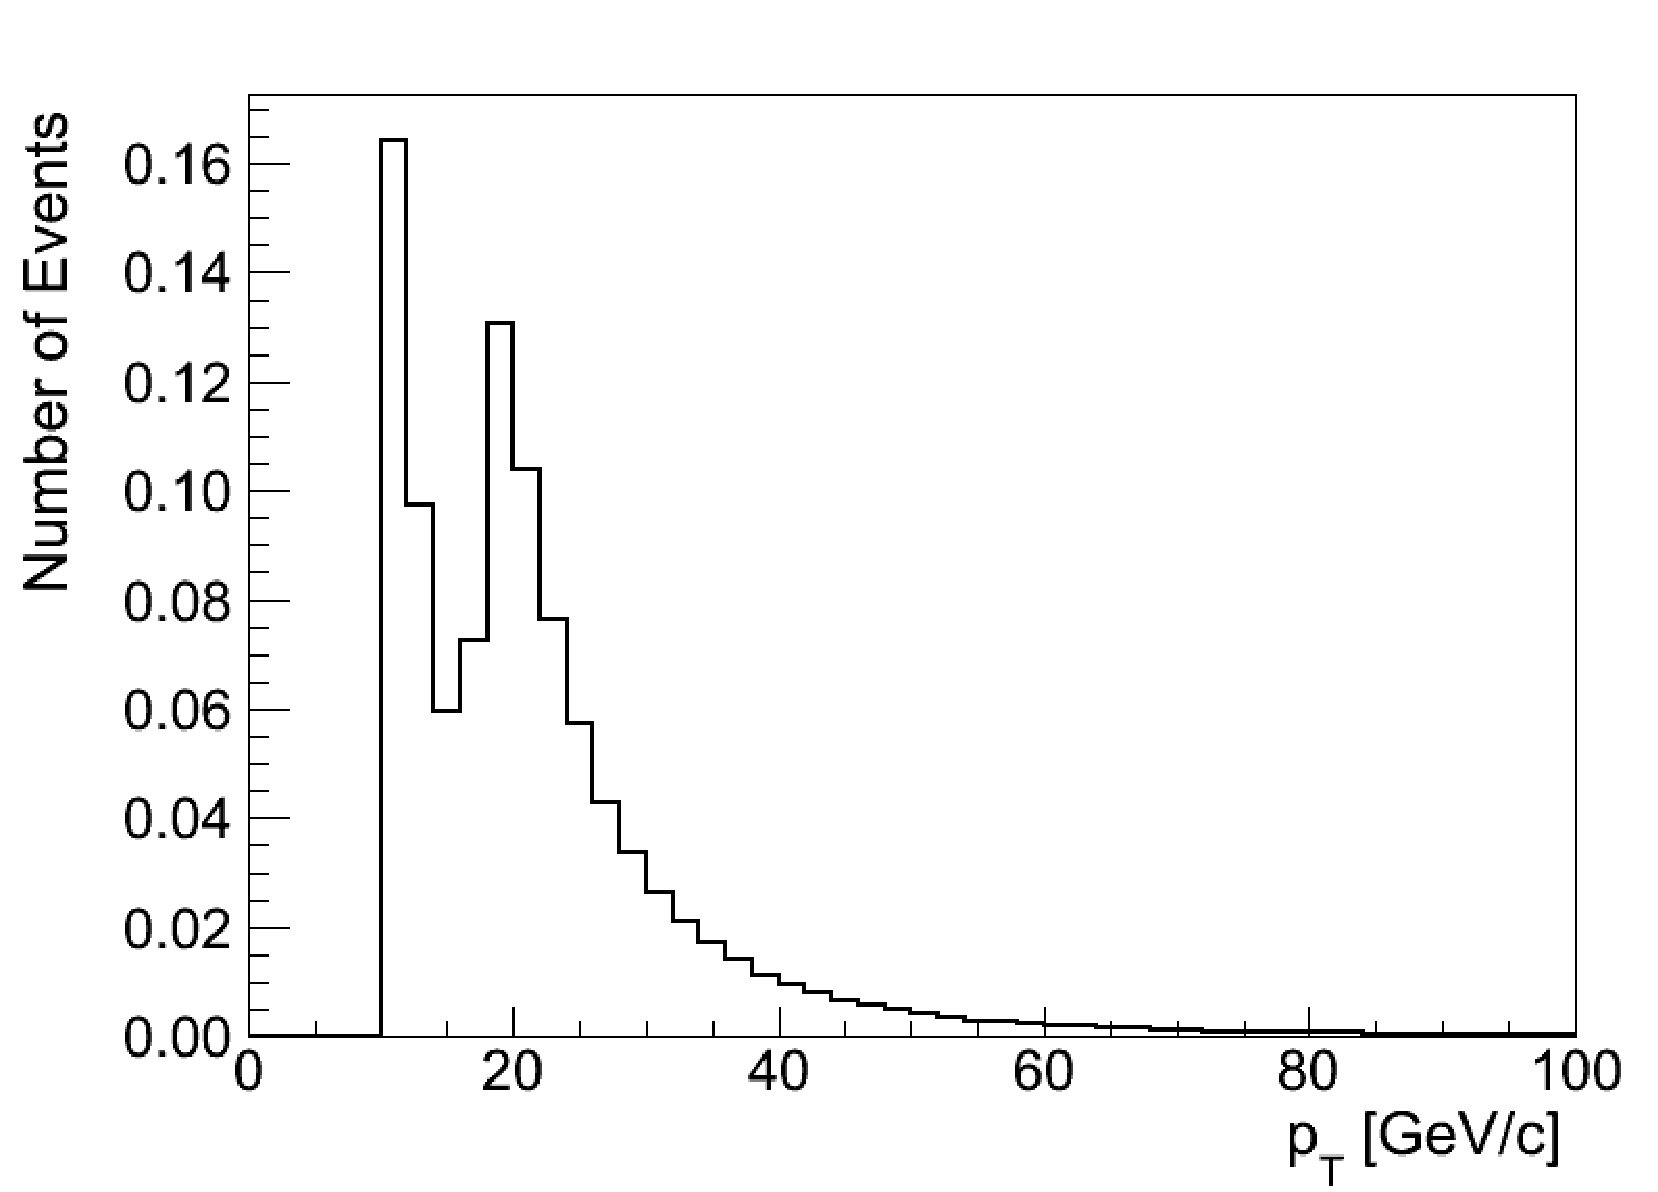
\includegraphics[width=0.45\textwidth]{figures/BkgPt_Source.pdf}}
\subfigure[Weighted]{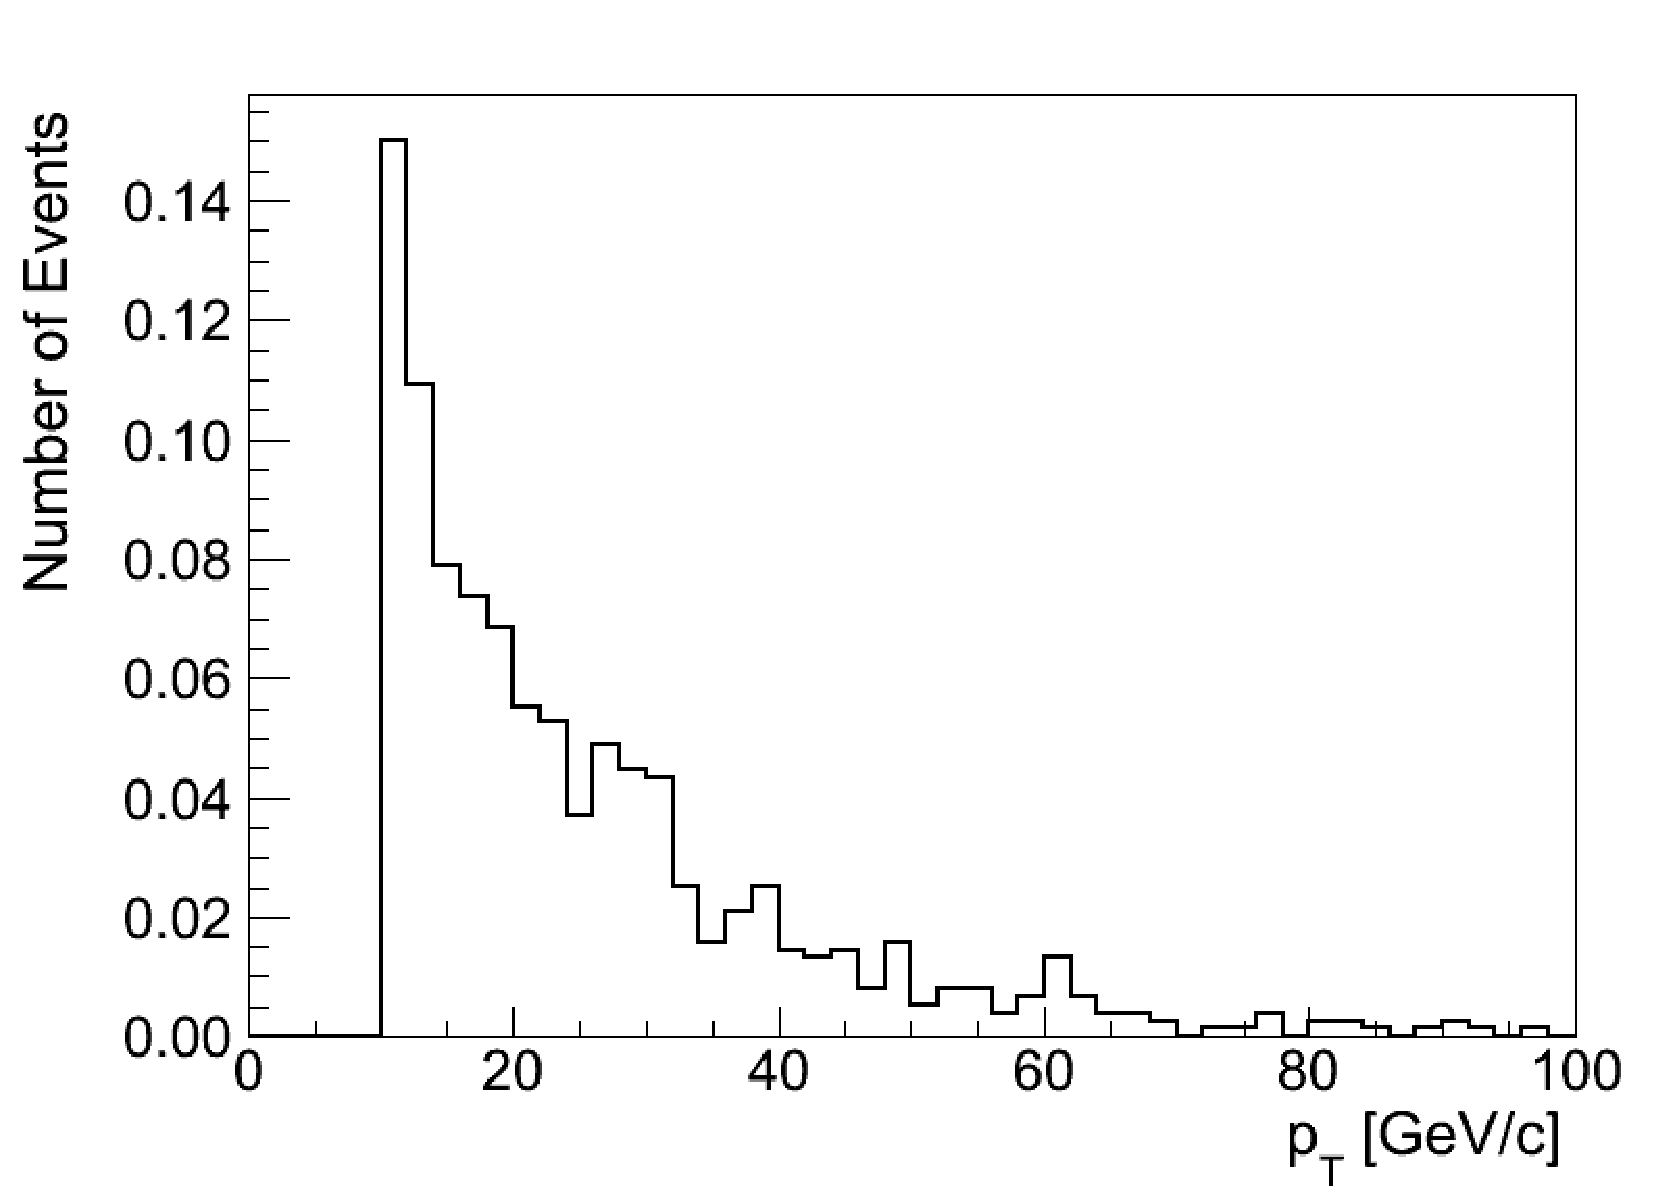
\includegraphics[width=0.45\textwidth]{figures/BkgPt_Target.pdf}}
\caption{The unweighted and weight \pt\ spectrum of the background electron training sample.}
\label{fig:BkgPtSpectrum}
\end{center}
\end{figure}

\section{Comparison of different MVA Methods}

To establish a baseline understanding of the input observables we begin with the standard projective likelihood method implemented in the TMVA toolkit. In Figure \ref{fig:ROC_TMVALHVsStandardLH} we compare the performance of this projective likelihood with the standard likelihood implemented in CMSSW \cite{EleLikelihood}, by plotting the signal efficiency versus background efficiency curve in the six different detector region and \pt\ bins. We observe that in all bins the re-trained projective likelihood performs similarly to the standard likelihood or in some cases better. This is expected since the standard likelihood has been built using Monte Carlo samples from an older release, which can exhibit differences to the current samples under study. 

\begin{figure}[!htbp]
\begin{center}
\subfigure[$10 \le \pt < 20$, $|\eta| < 1.0$]{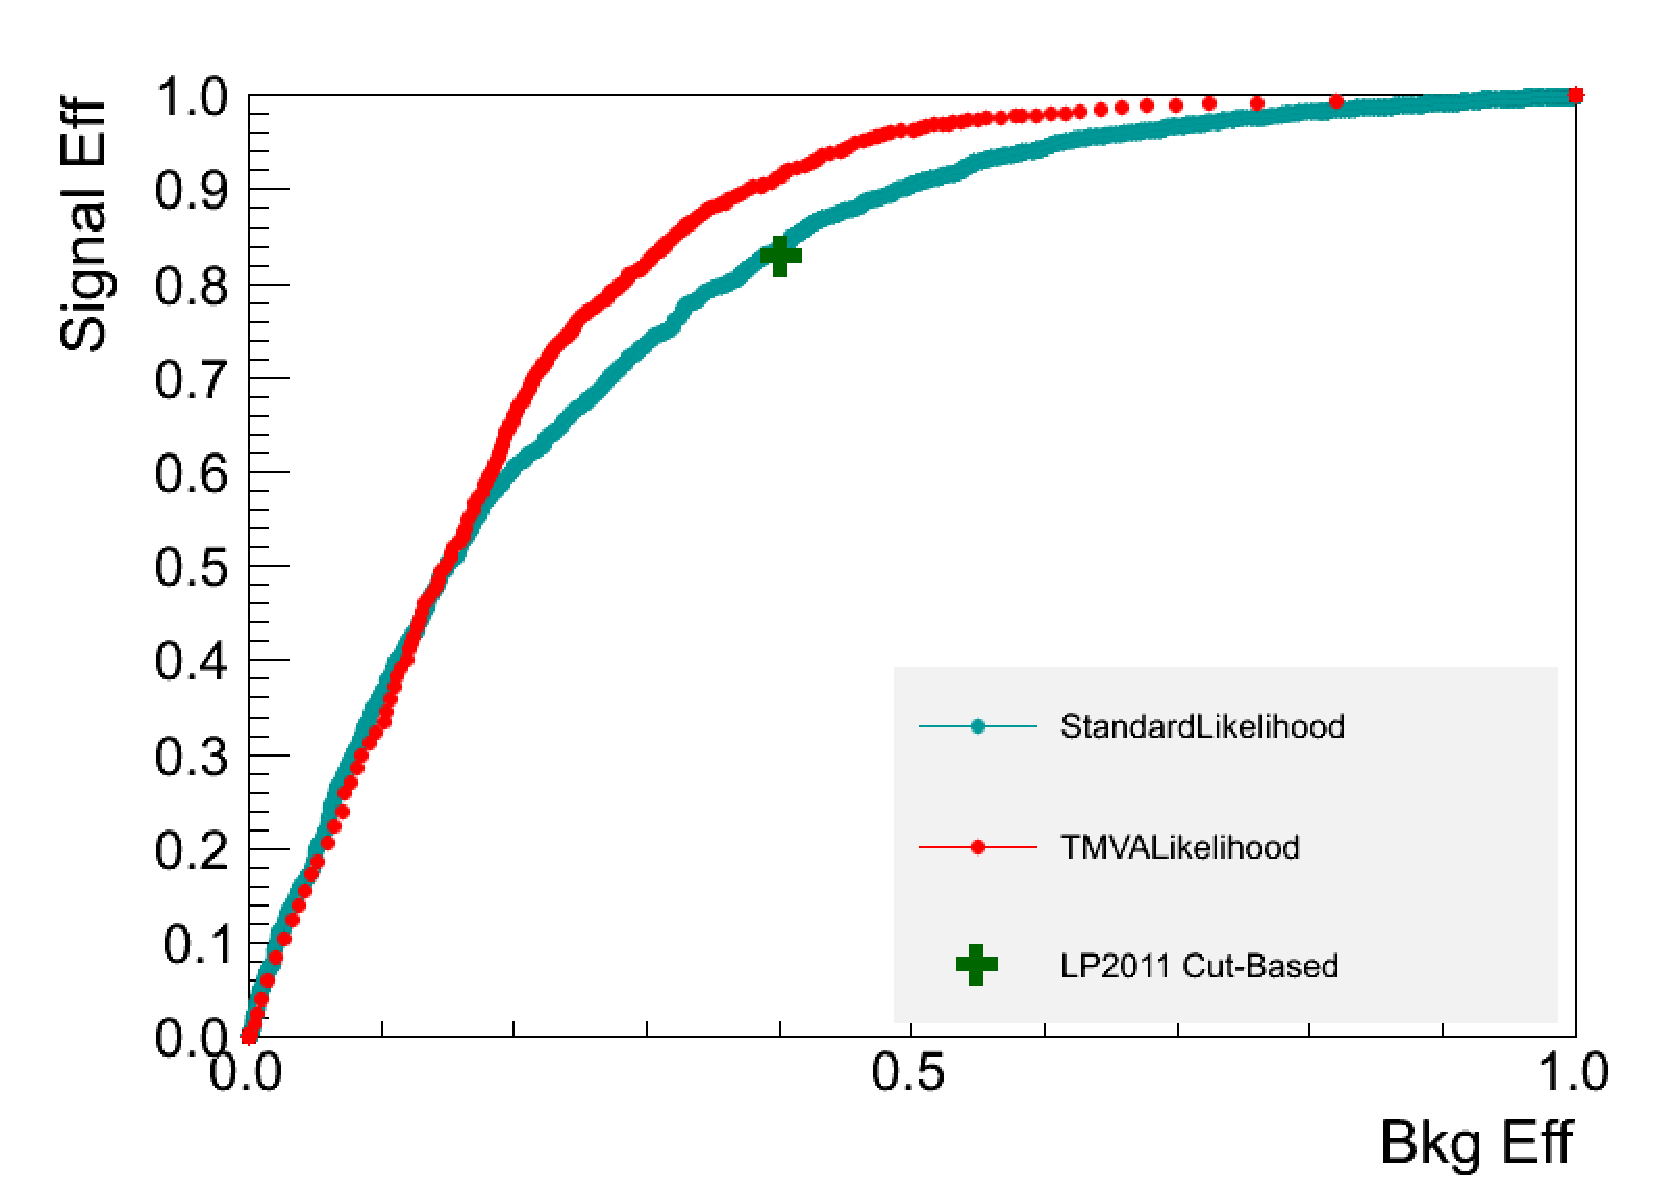
\includegraphics[width=0.45\textwidth]{figures/ROCGraphs_ElectronIDMVA_TMVALHVsStandardLH_Subdet0LowPt.pdf}}
\subfigure[$10 \le \pt < 20$, $1.0 \le |\eta| < 1.5$]{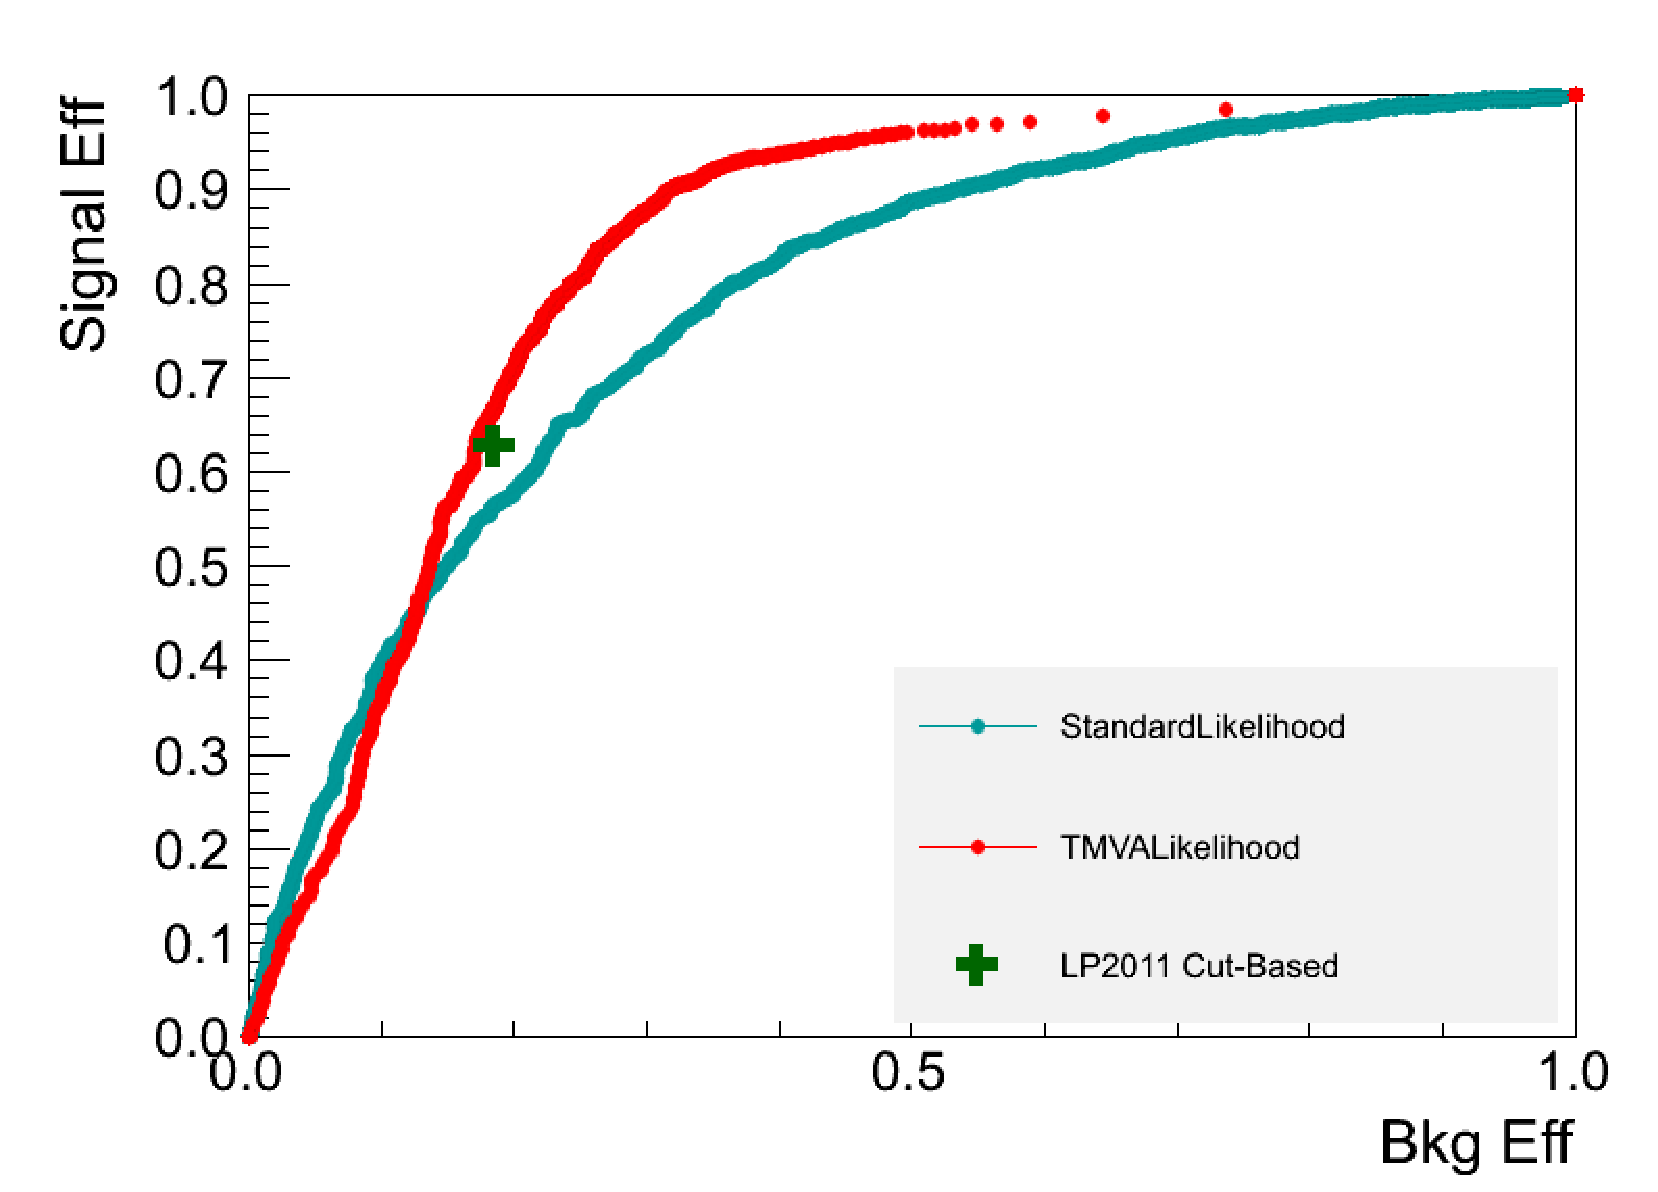
\includegraphics[width=0.45\textwidth]{figures/ROCGraphs_ElectronIDMVA_TMVALHVsStandardLH_Subdet1LowPt.pdf}}
\subfigure[$10 \le \pt < 20$, $1.5 \le |\eta| < 2.5$]{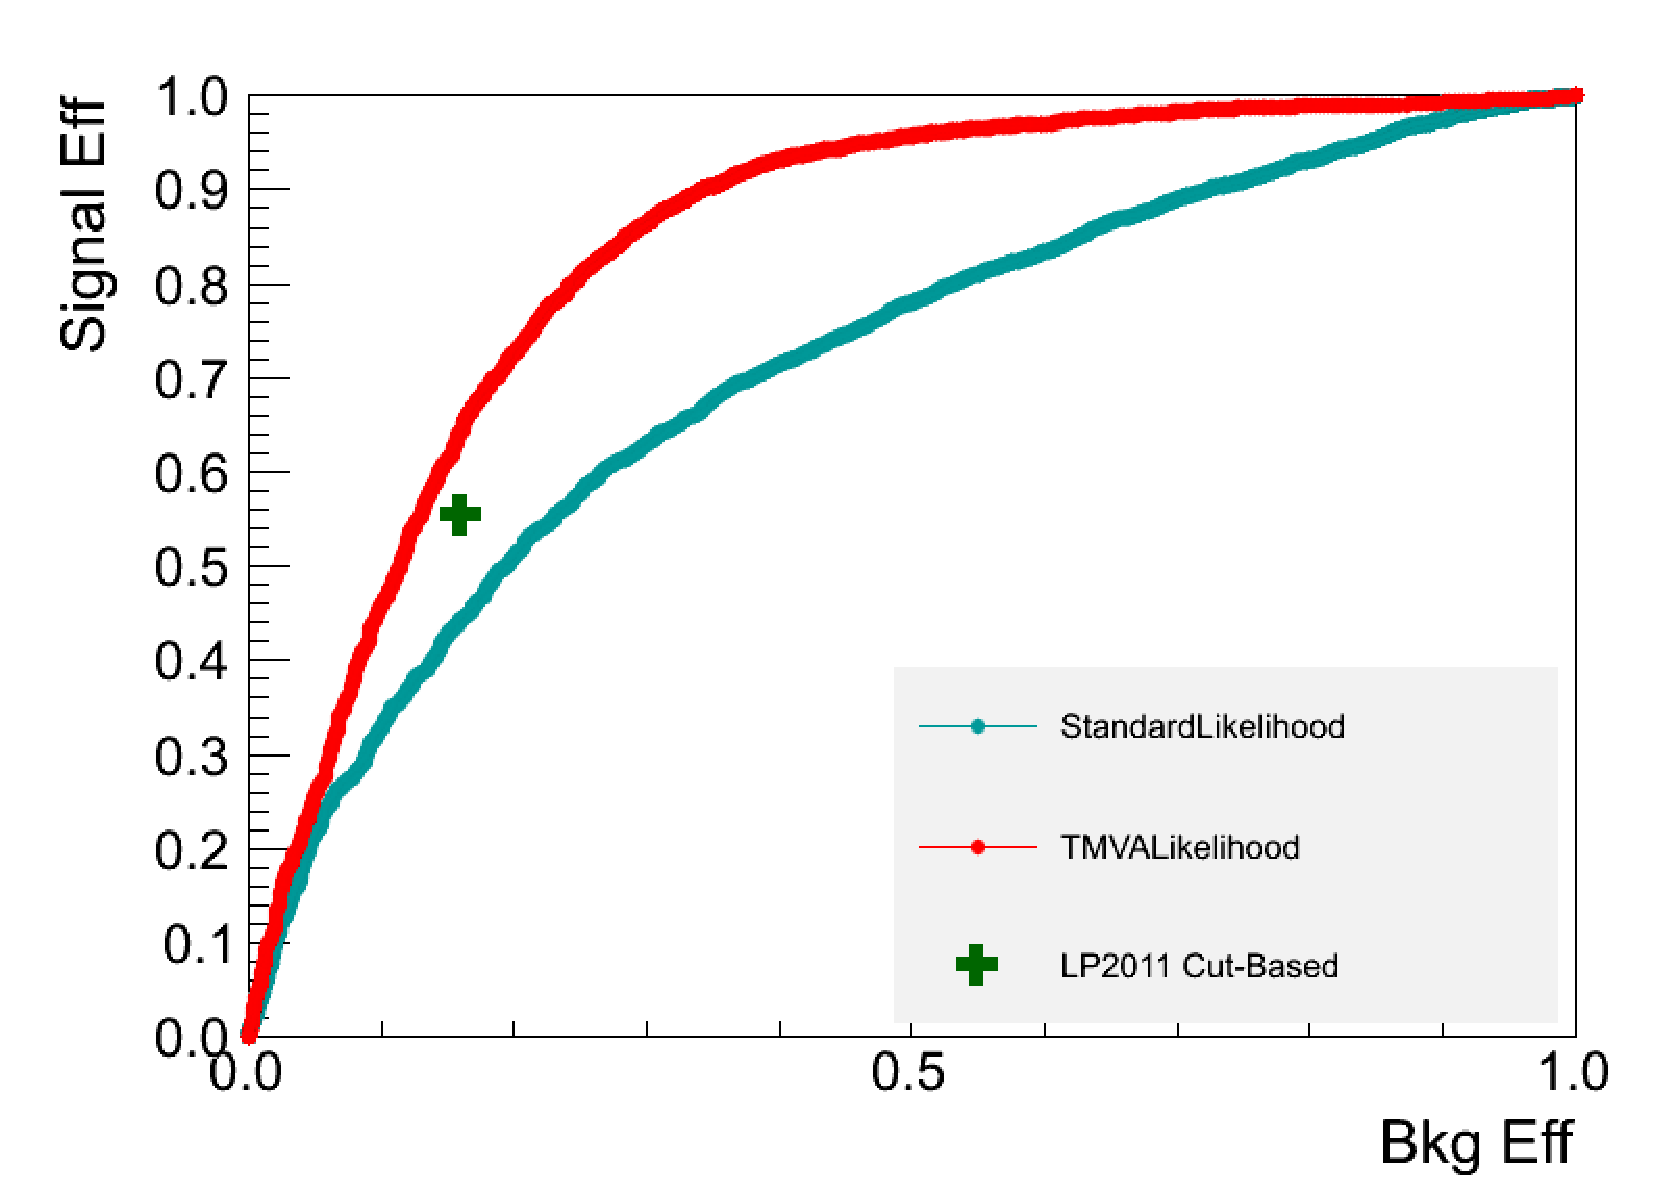
\includegraphics[width=0.45\textwidth]{figures/ROCGraphs_ElectronIDMVA_TMVALHVsStandardLH_Subdet2LowPt.pdf}}
\subfigure[$\pt \ge 20$, $|\eta| < 1.0$]{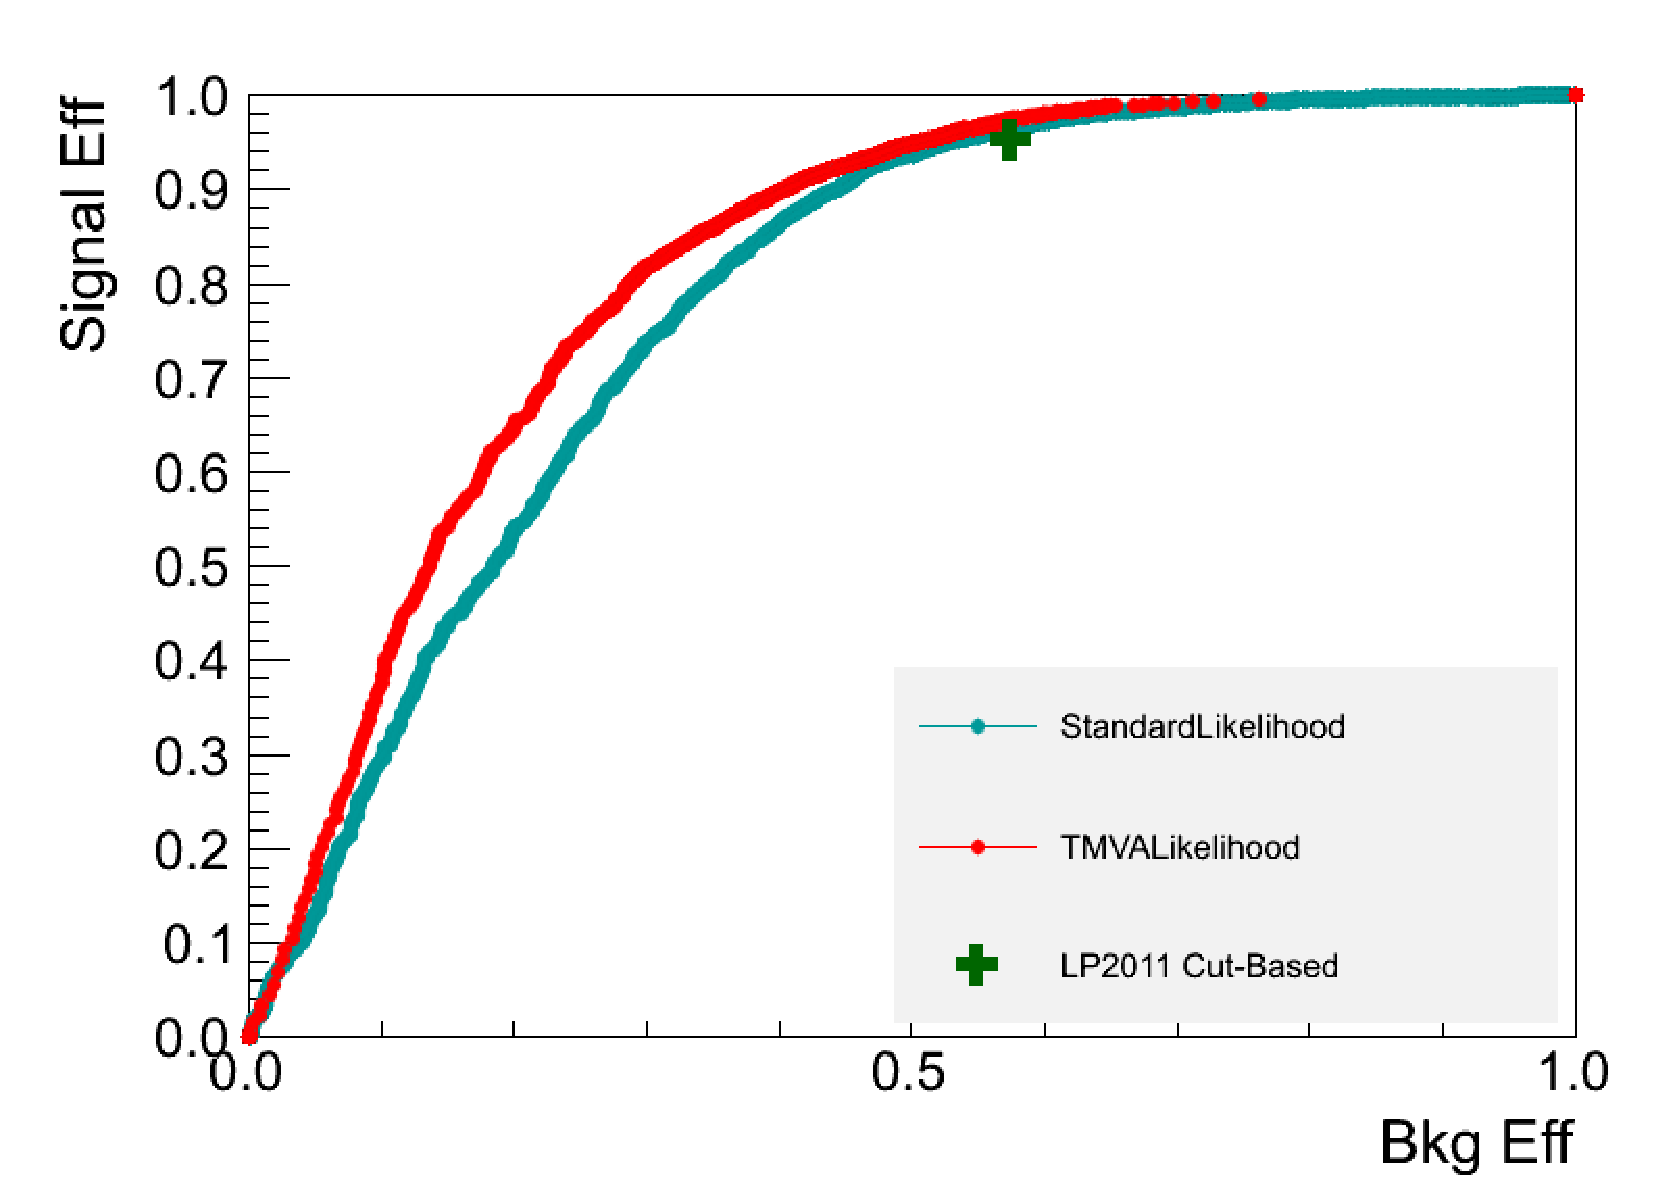
\includegraphics[width=0.45\textwidth]{figures/ROCGraphs_ElectronIDMVA_TMVALHVsStandardLH_Subdet0HighPt.pdf}}
\subfigure[$\pt \ge 20$, $1.0 \le |\eta| < 1.5$]{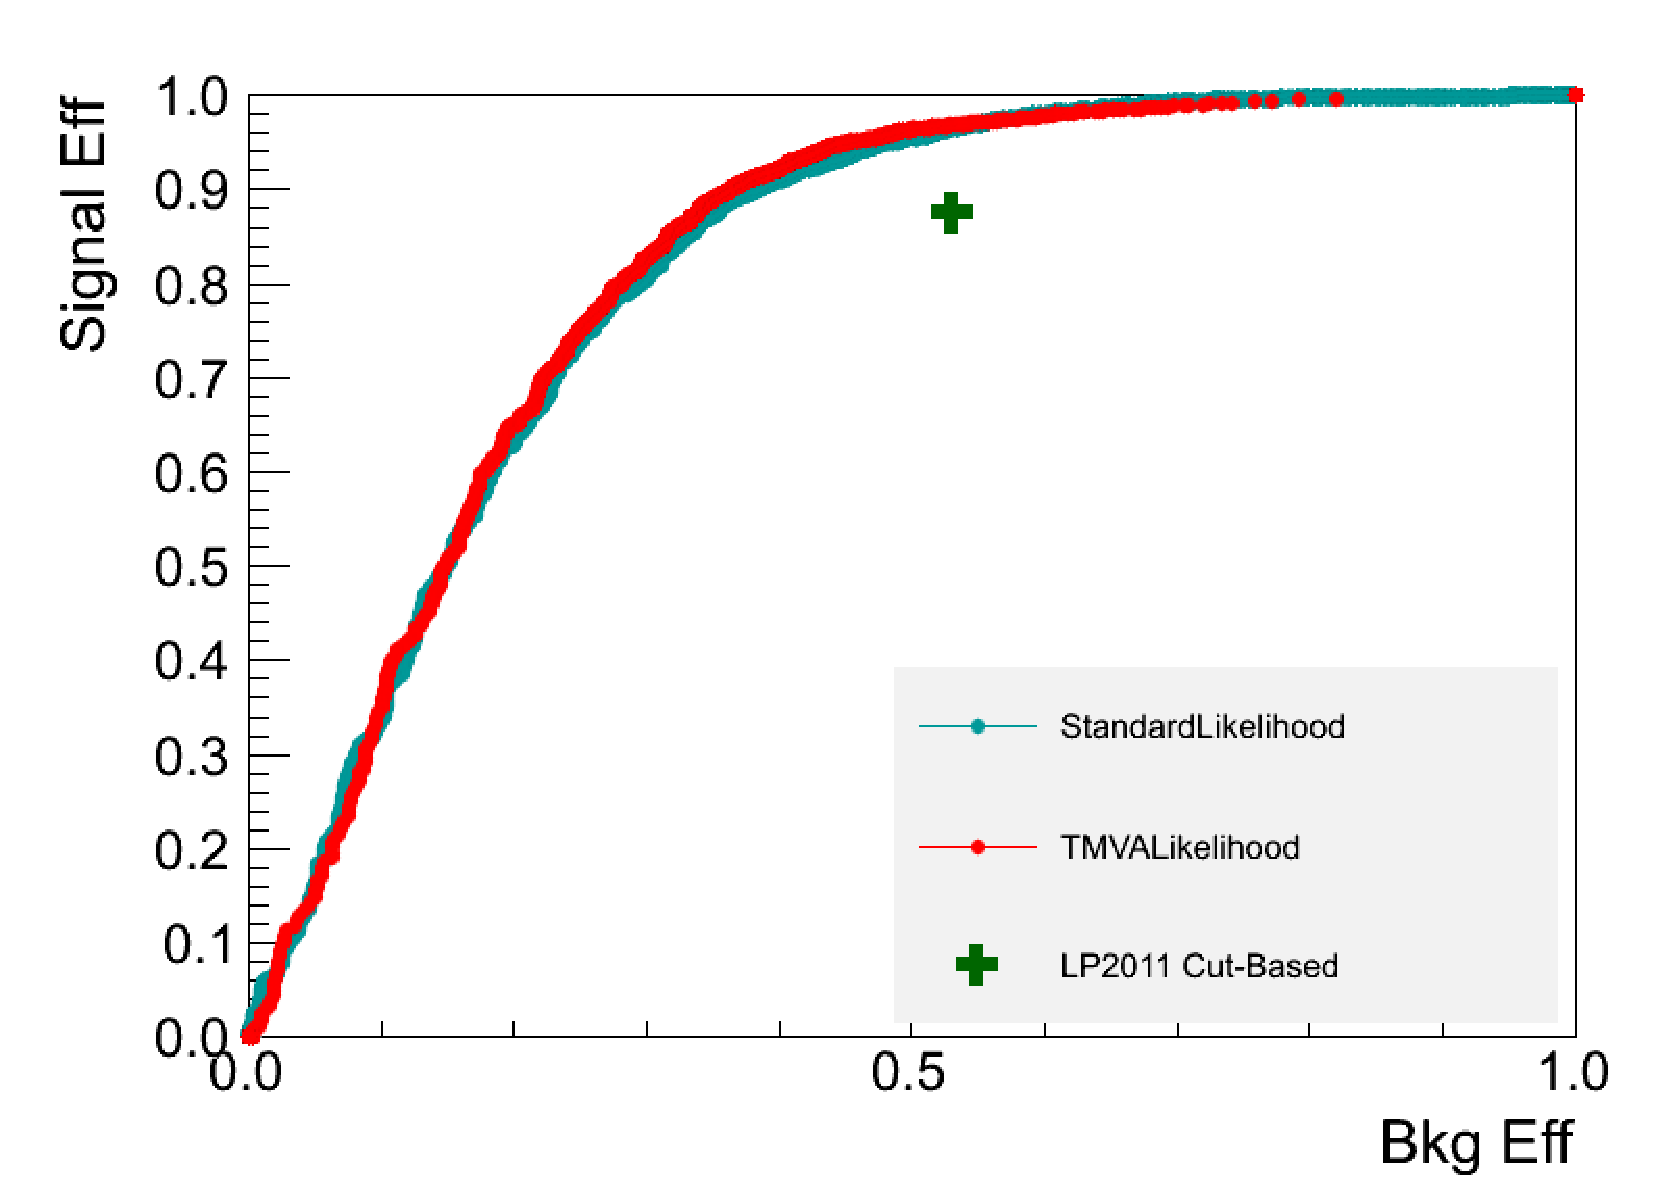
\includegraphics[width=0.45\textwidth]{figures/ROCGraphs_ElectronIDMVA_TMVALHVsStandardLH_Subdet1HighPt.pdf}}
\subfigure[$\pt \ge 20$, $1.5 \le |\eta| < 2.5$]{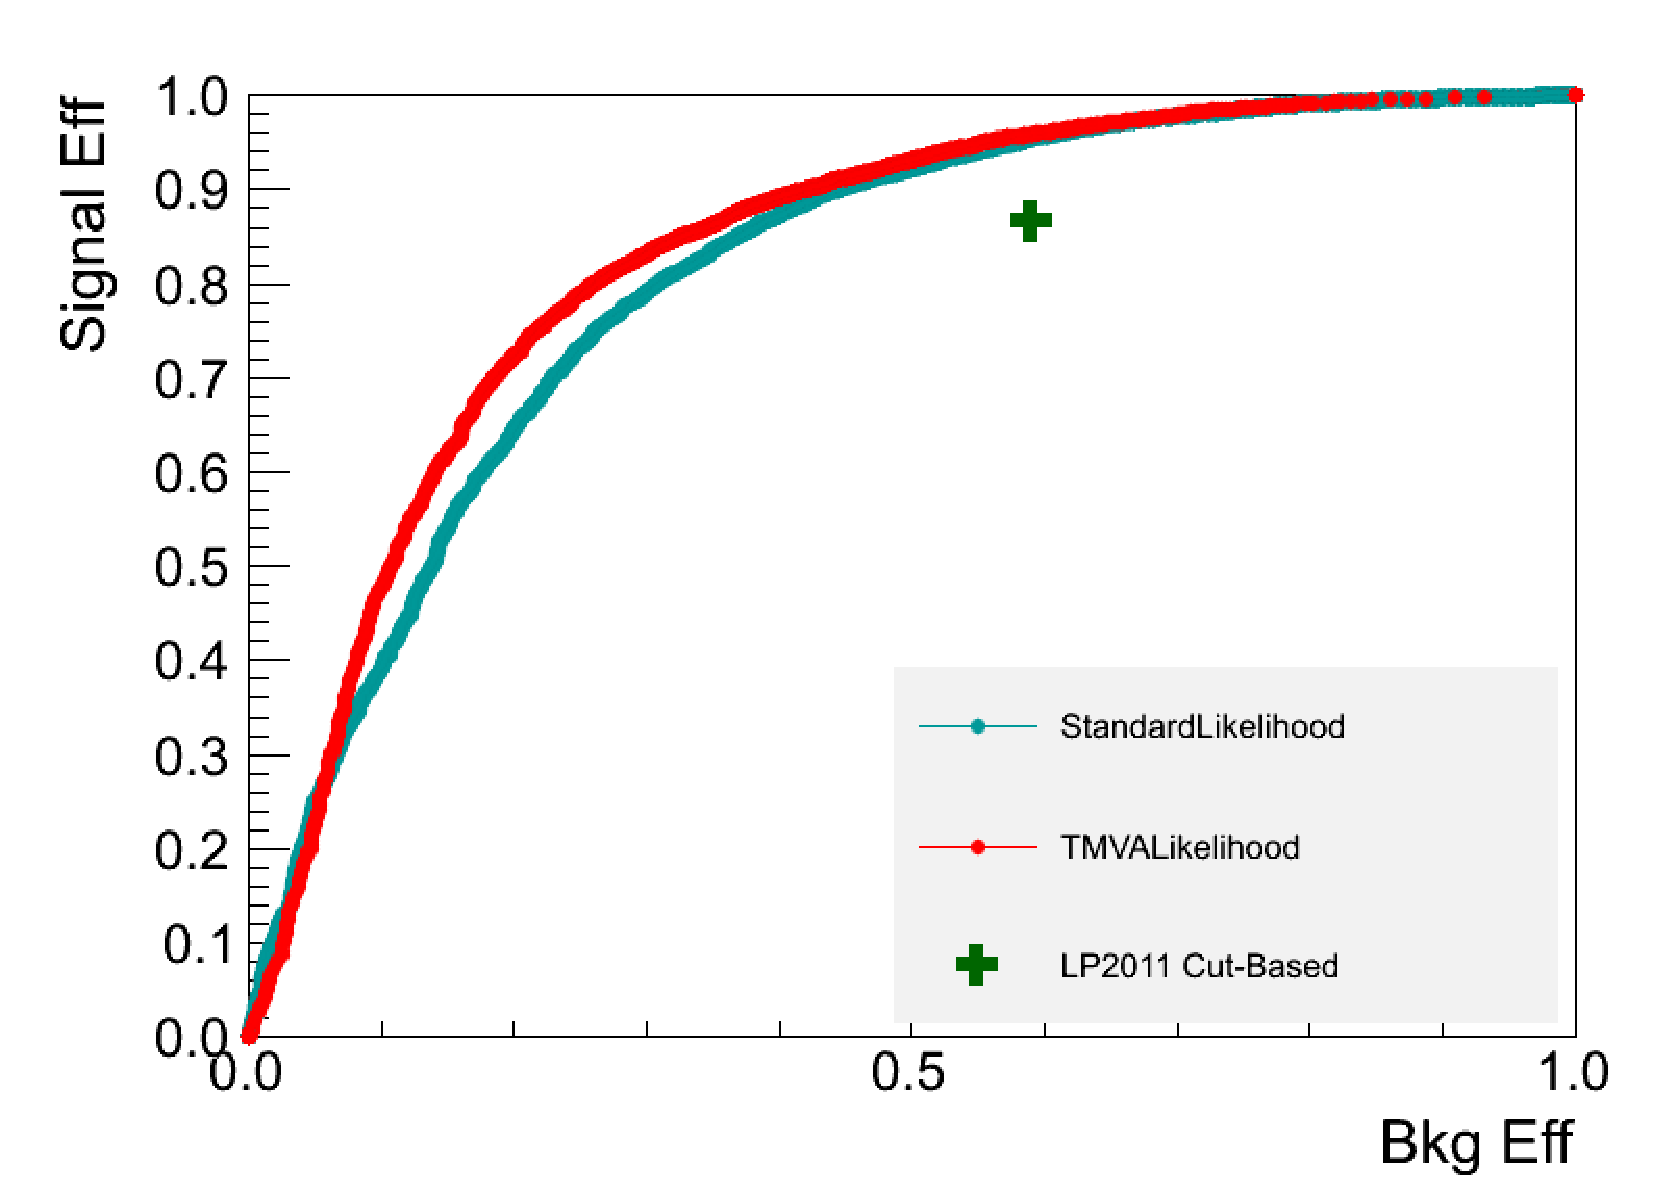
\includegraphics[width=0.45\textwidth]{figures/ROCGraphs_ElectronIDMVA_TMVALHVsStandardLH_Subdet2HighPt.pdf}}
\caption{Comparison of the ROC curves for the projective likelihood using the TMVA implementation and the likelihood implemented in CMSSW.}
\label{fig:ROC_TMVALHVsStandardLH}
\end{center}
\end{figure}

Next, we compare the performance between the projective likelihood and the boosted decision tree (BDT), one of the standard multivariate discrimination methods demonstrated to have robust performance in other contexts. In Figure \ref{fig:ROC_BDTvsLH} we show the signal efficiency versus background efficiency curves for the projective likelihood and the BDT for the electrons with $10 \le \pt < 20$ and $|\eta| < 1.0$. We observe that for every choice of working point the BDT has slightly better performance than the projective likelihood. For the same signal efficiency, we reject approximately $10\%$ more background. 

\begin{figure}[!htbp]
\begin{center}
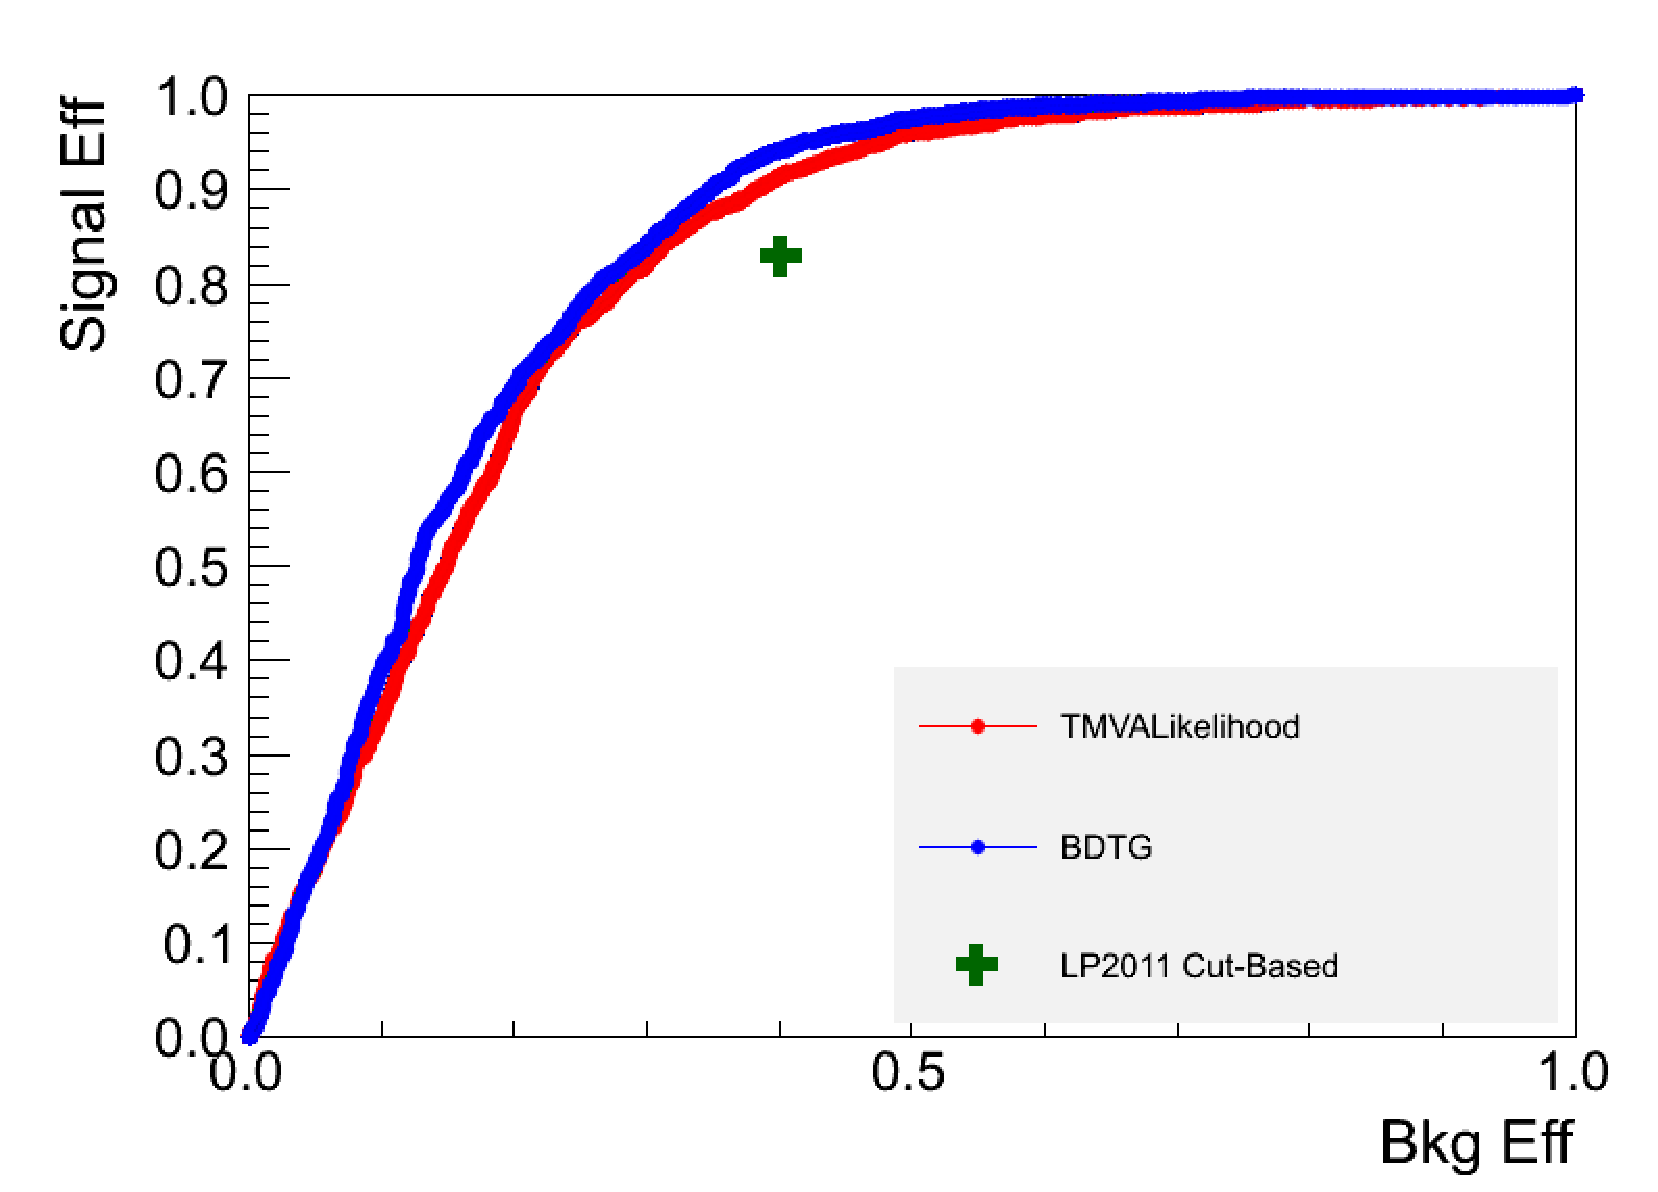
\includegraphics[width=0.45\textwidth]{figures/ROCGraphs_ElectronIDMVA_BDTvsLH_Subdet0LowPt.pdf}
\caption{Comparison of the ROC curves for projective likelihood and boosted decision tree (BDT)
for electrons in the bin with $10 \le \pt < 20$ and $|\eta| < 1.0$. The working point used for 
the cut based electron selection is shown in the green cross.}
\label{fig:ROC_BDTvsLH}
\end{center}
\end{figure}

Next we study the performance for a variety of different multivariate discrimination methods implemented in TMVA. Two variations of the boosted decision tree is tested, implementing two different boosting methods. In the adaptive boost method (BDT), an exponential loss function is used to parameterize the degree of learning while in the gradient boost method (BDTG) a binomial log likelihood loss function is used which is expected to be more robust in the presence of outliers in the training sample. Two neural network implementations (MLP and MLPBNN) are tested as well as the k-nearest neighbour (kNN) method. From Figure \ref{fig:ROC_CompareAllMVAMethods} we observe that the gradient boost version of the BDT and the MLPBNN performs the best. In practice since the BDT training is much faster, in subsequent results we only report results for the BDTG classifier. 

\begin{figure}[!htbp]
\begin{center}
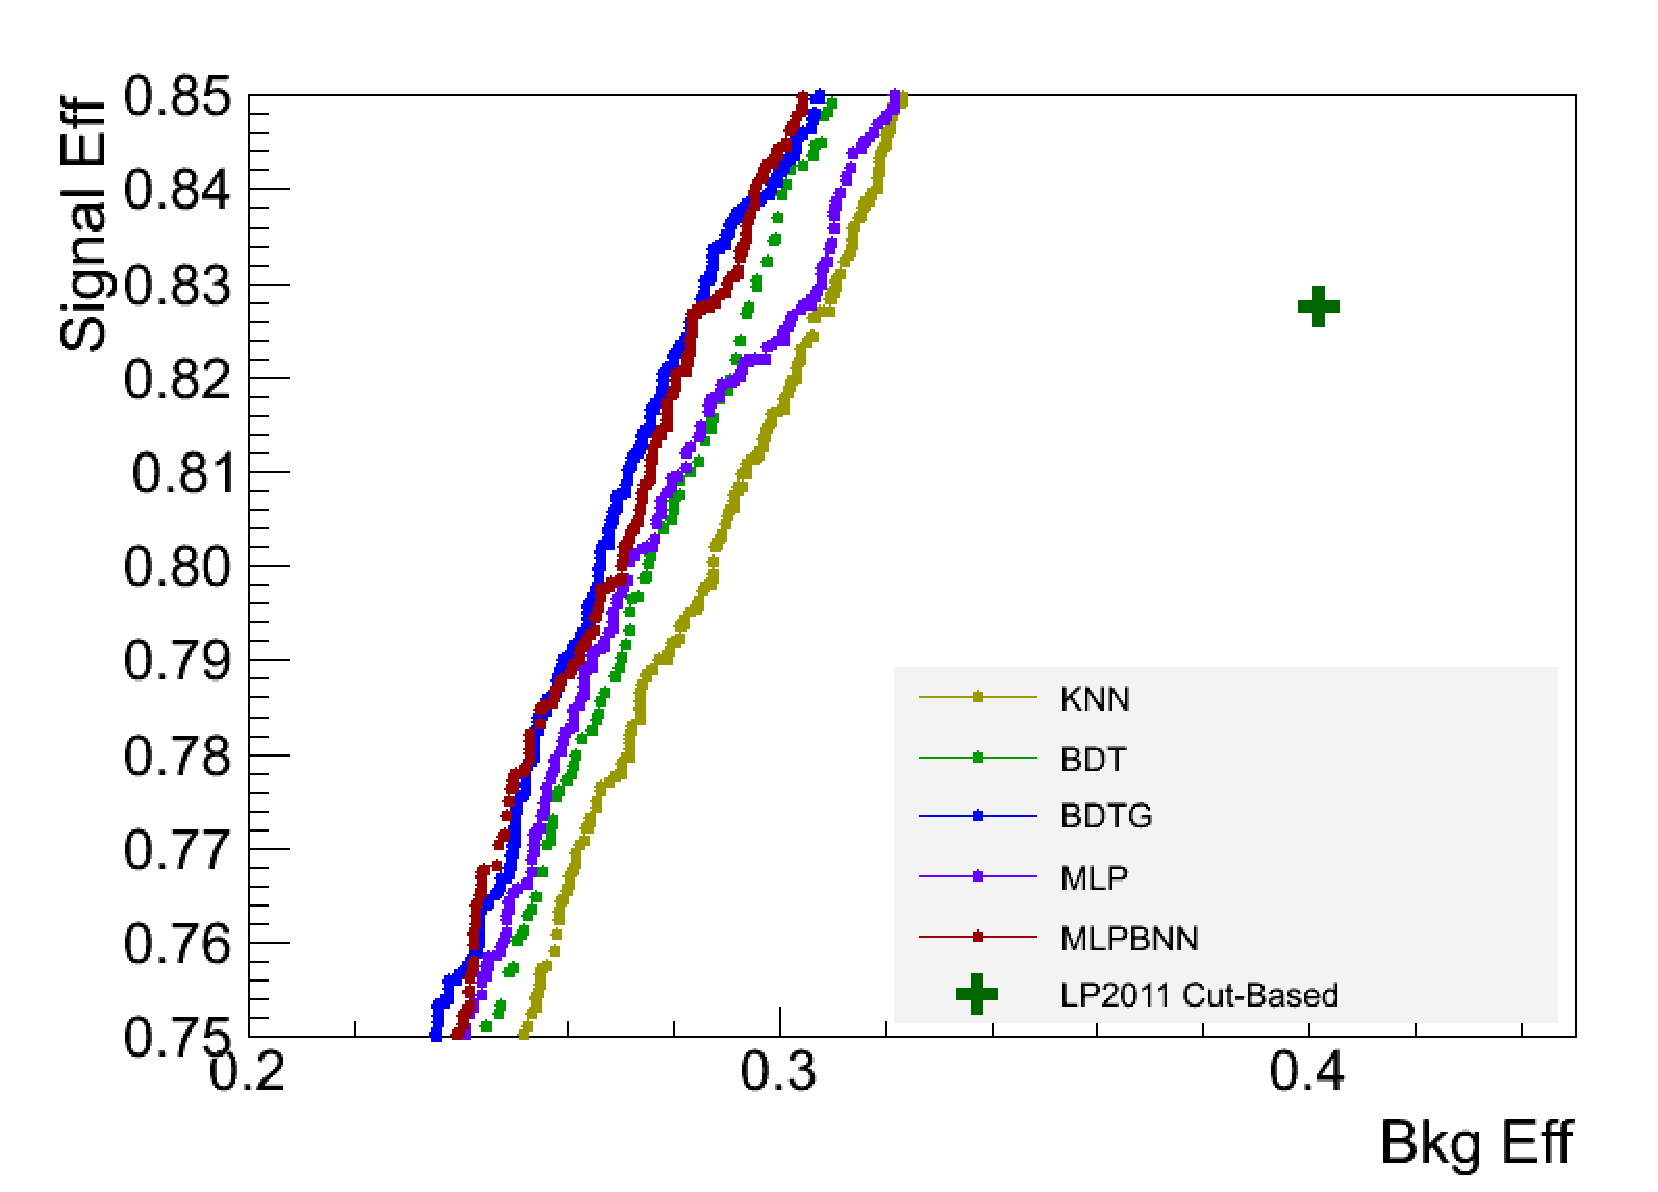
\includegraphics[width=0.45\textwidth]{figures/ROCGraphs_ElectronIDMVA_CompareAllMVAMethods_Subdet0LowPt.pdf}
\caption{Comparison of the ROC curves for a number of different multivariate discriminators for electrons
in the bin with $10 \le \pt < 20$ and $|\eta| < 1.0$. The working point used for the cut based electron
selection is shown in the green cross.}
\label{fig:ROC_CompareAllMVAMethods}
\end{center}
\end{figure}

Some attempt was made to tune the training parameters of the BDTG algorithm on the current training sample. It was observed that with the $4.0.7$ version of TMVA, the bagging option was causing a degradation of performance by roughly $10\%$ and is therefore turned off. The number of trees used in the training, the maximum depth of the trees, and the minimum number of events in one leaf node were found to have no effect on the performance with the current training sample. 

Finally, we investigated two different methods to combine the results of different multivariate discriminators. In the first method we construct a new discriminator formed by the product of the signal likelihood with an assumed signal to background ratio of $1$ of each MVA discriminator. Using this ``combined'' discriminator generally does not yield any improvements but rather follows the performance of the best single discriminator. In the second method we feed each MVA discriminator output as input to train a new MVA discriminator, typically referred to as the committee method. This method is expected to yield improved performance if the different MVA discriminators are not too highly correlated. We observe worse performance with the current training sample, likely due to the limited size of our training samples. These conclusions are demonstrated in Figure \ref{fig:ROC_CompareCombinedMVA}.

\begin{figure}[!htbp]
\begin{center}
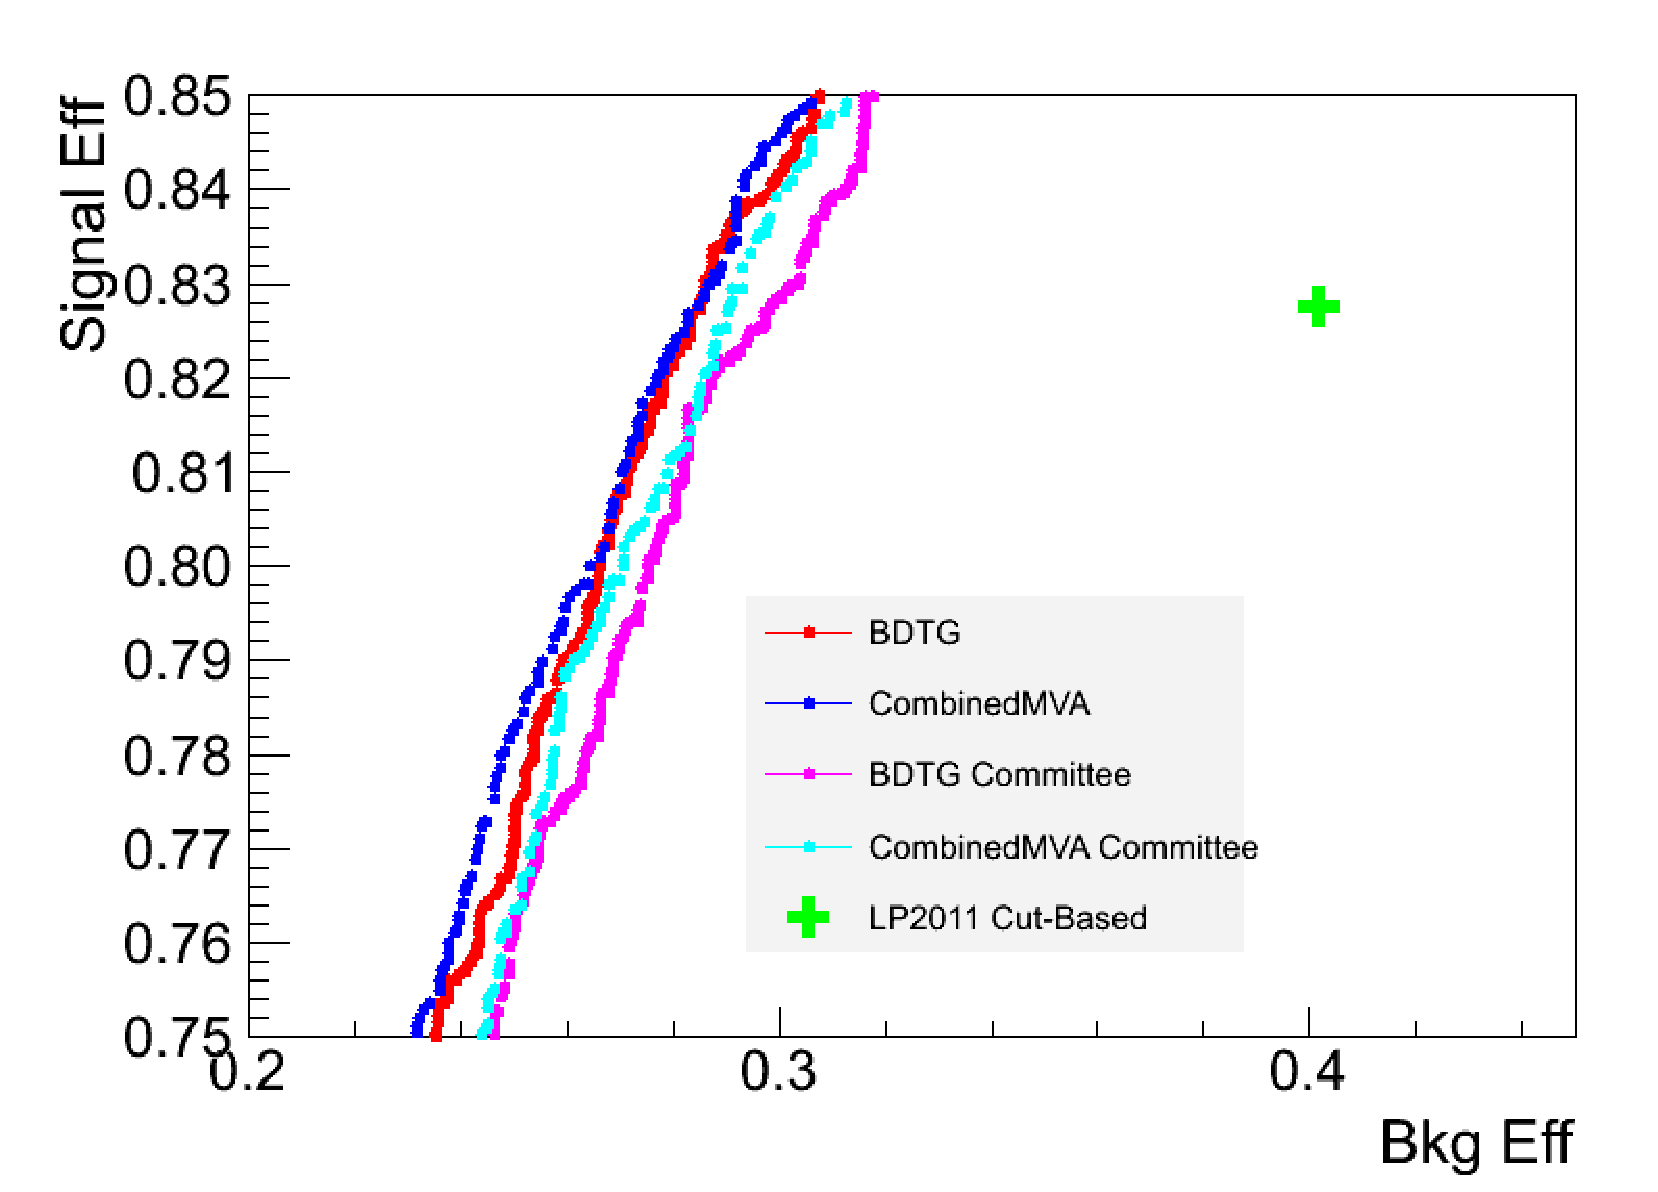
\includegraphics[width=0.45\textwidth]{figures/ROCGraphs_ElectronIDMVA_CompareCombinedMVA_Subdet0LowPt.pdf}
\caption{Comparison of the ROC curves for a number of different multivariate discriminators for electrons
in the bin with $10 \le \pt < 20$ and $|\eta| < 1.0$. The working point used for the cut based electron
selection is shown in the green cross.}
\label{fig:ROC_CompareCombinedMVA}
\end{center}
\end{figure}


\section{Improvement Through Additional Observables}
Having established the BDTG method as the best available multivariate discriminator, we investigate performance gains as additional observables are added to the training. We add additional observables in two stages. In the first stage we add the following discriminating variables:

\begin{itemize}
  \item $E_{\mathrm{supercluster}} / p_{\mathrm{gsf\ track}}$,
  \item $E_{\mathrm{seed\ cluster}} / p_{\mathrm{out}}$,
  \item $E_{\mathrm{seed\ cluster}} / p_{\mathrm{in}}$.
\end{itemize}

Since there are no observables related to the impact parameter, this version is intended to be more generally applicable to lepton analyses.

In the second stage we add these additional impact parameter observables to the MVA training:

\begin{itemize}
  \item $d_{0}$,
  \item 3D impact parameter,
  \item 3D impact parameter significance.
\end{itemize}

This MVA discriminator is expected to give better performance for the \hww\ analysis, but may be not optimal for selecting leptons resulting from the decay of a particle with a naturally larger decay length, such as tau leptons. 

The comparison of the baseline MVA discriminator with these two improved MVA discriminators is shown in Figure \ref{fig:ROC_BaselineV1V2} for the bin with $10 \le \pt < 20$ and $|\eta| < 1.0$. We observe that adding the additional variables without impact parameter information adds roughly $15\%$ in additional background rejection, and adding the impact parameter observables gives another $25\%$ improvement on top. 

\begin{figure}[!htbp]
\begin{center}
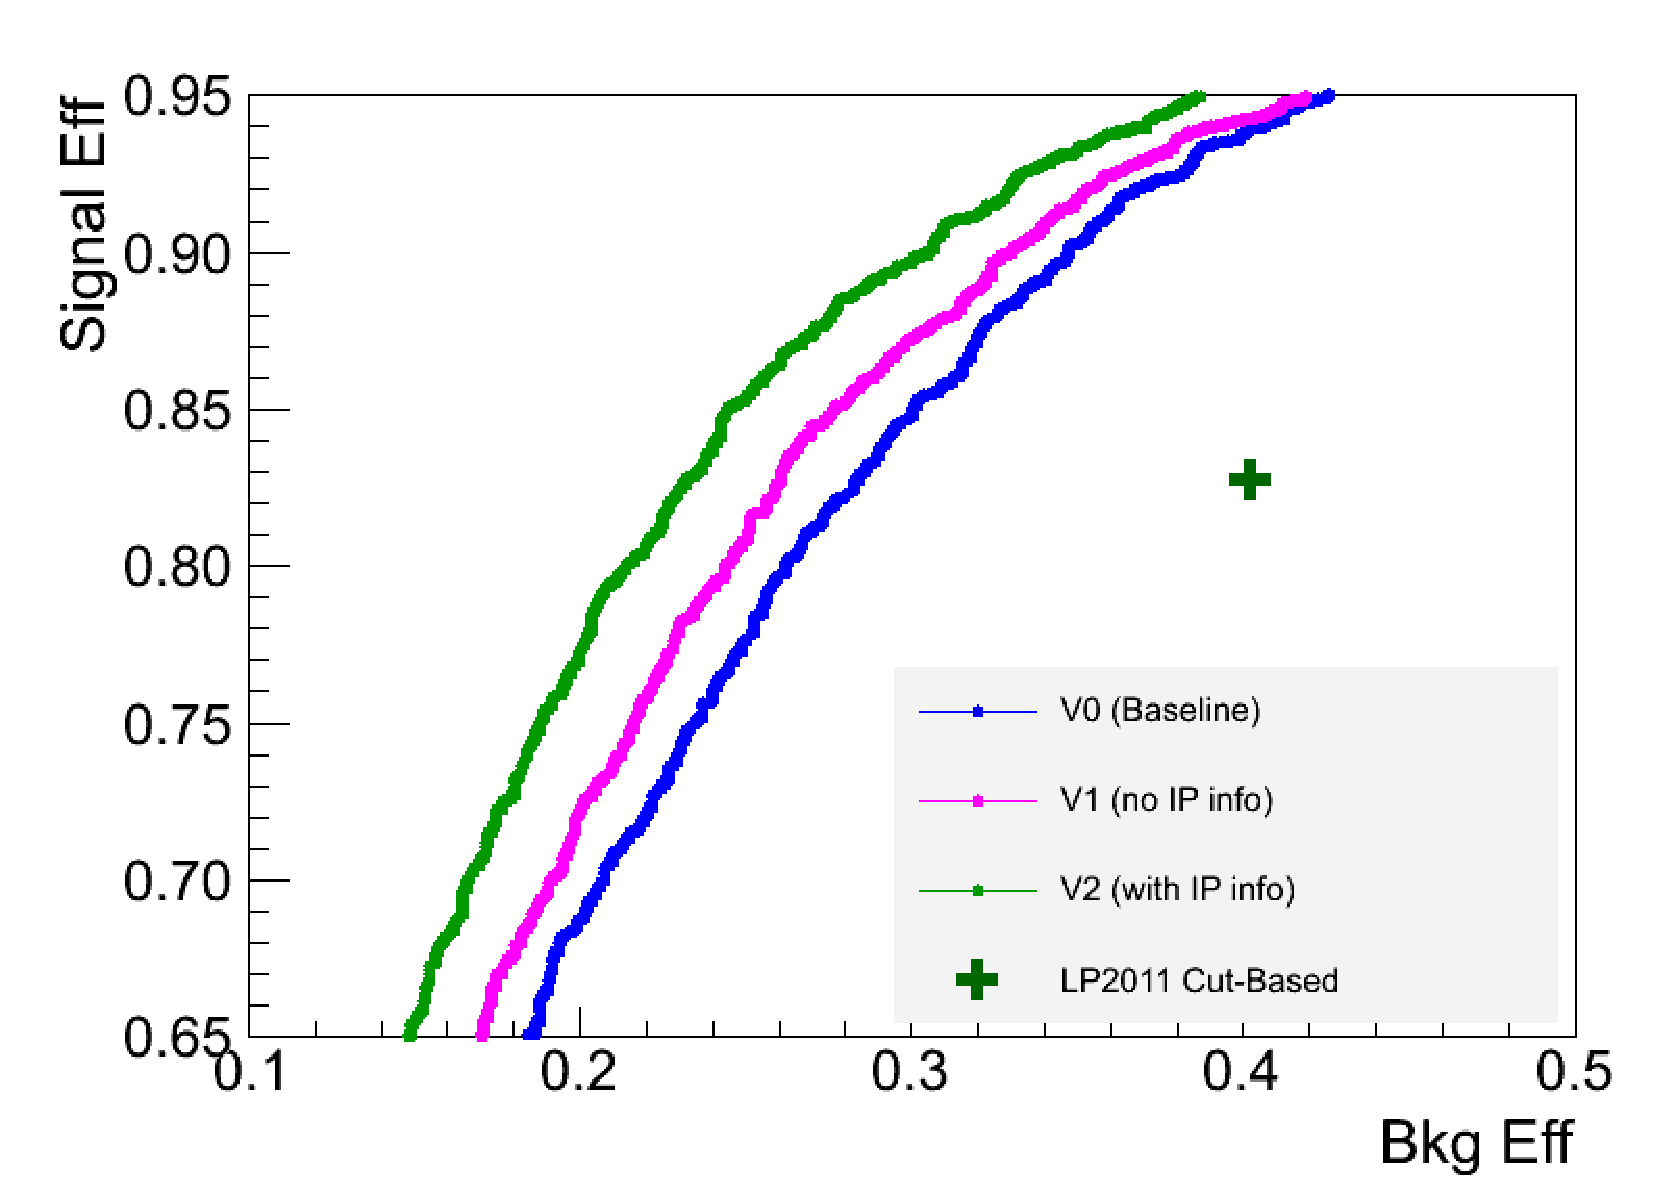
\includegraphics[width=0.45\textwidth]{figures/ROCGraphs_ElectronIDMVA_BaselineV1V2_Subdet0LowPt.pdf}
\caption{Comparison of the ROC curves for the baseline BDT discriminator and 
the two improved BDT discriminators which make use of additional observables. 
The working point used for the cut based electron selection is shown in the green cross.}
\label{fig:ROC_BaselineV1V2}
\end{center}
\end{figure}

The same trend is exhibited in the remaining five kinematic bins shown collectively in Figure \ref{fig:ROC_Performance}. We choose new working points for the electron selection which give the same signal efficiency as the cut based selection used for the Lepton Photon 2011 \hww\ analysis. Using these working points, we reject approximately $40\%$ to $50\%$ more background than the cut based selection. For the low $\pt$ electrons, the addition of the impact parameter gives an improvement of roughly $20\%$, while for high $\pt$ electrons it does not give any significant improvement. 

\begin{figure}[!htbp]
\begin{center}
\subfigure[$10 \le \pt < 20$, $|\eta| < 1.0$]{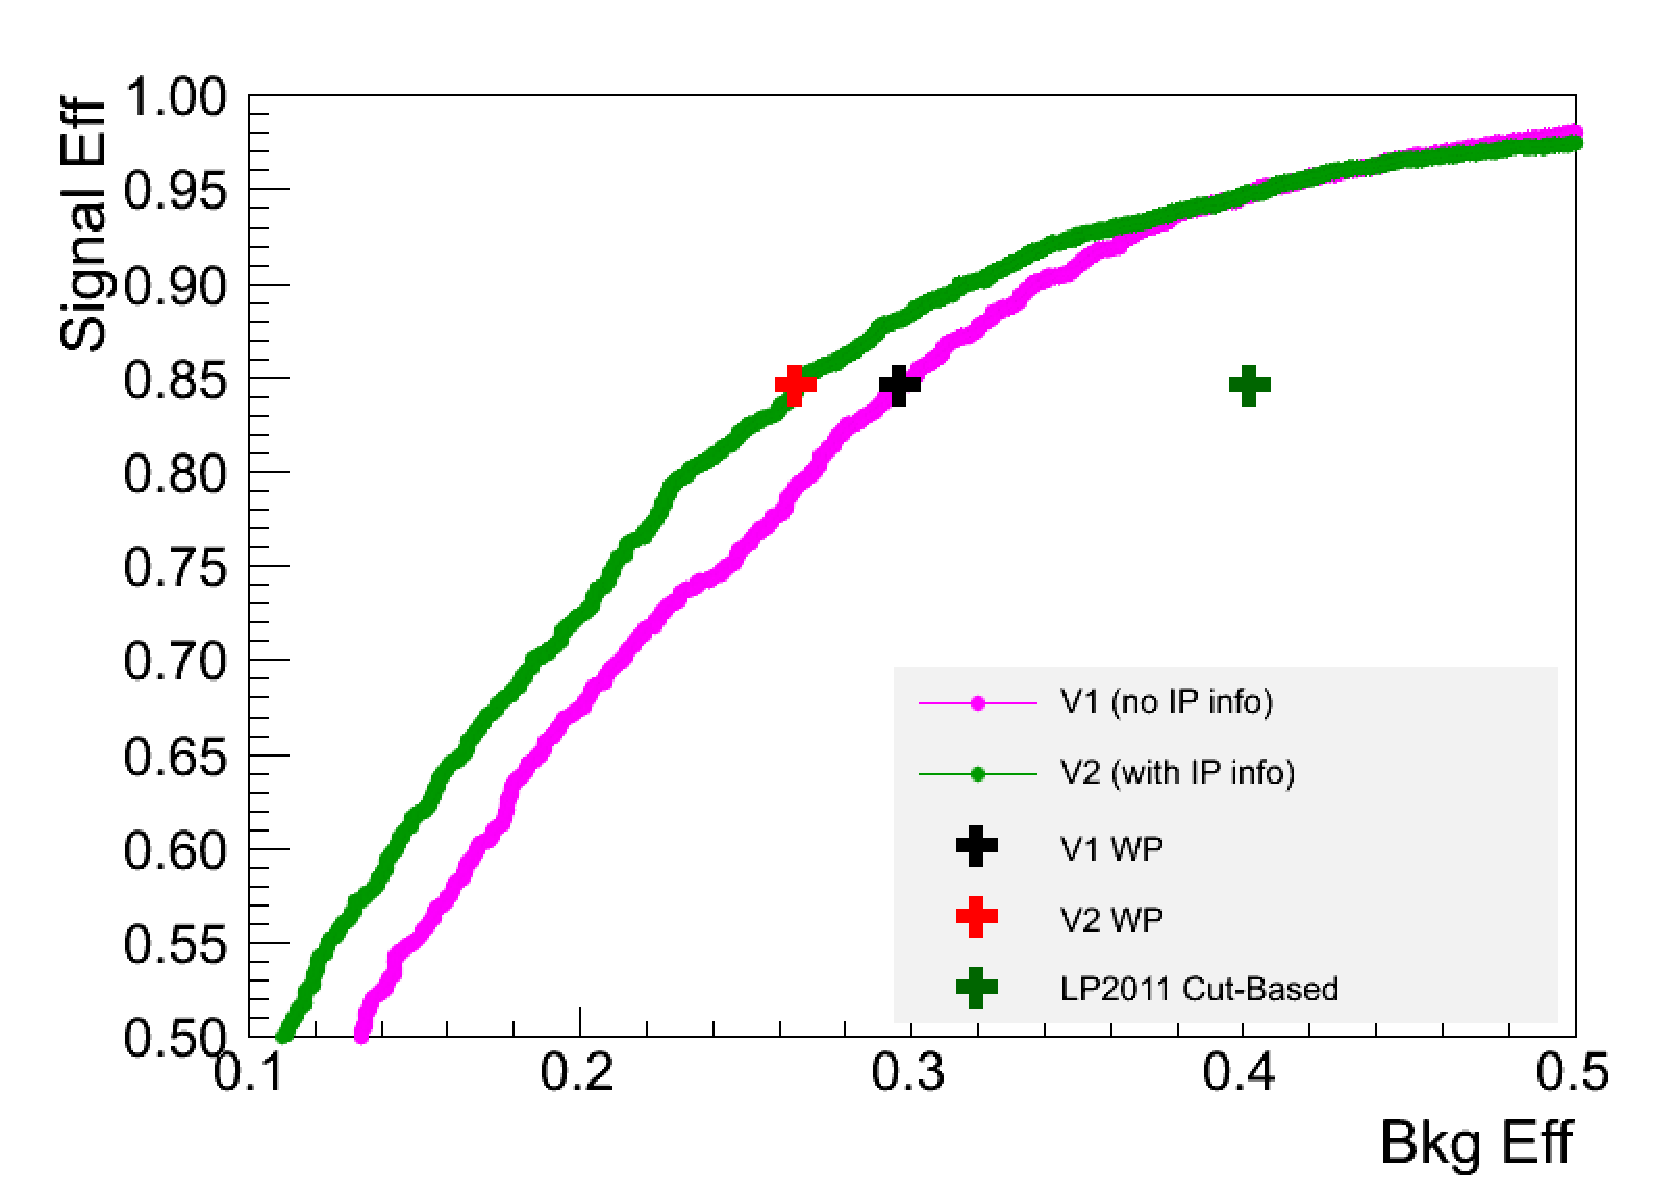
\includegraphics[width=0.45\textwidth]{figures/ROCGraphs_ElectronIDMVA_WithAndWithoutIPInfoSubdet0LowPt_HWW115.pdf}}
\subfigure[$10 \le \pt < 20$, $1.0 \le |\eta| < 1.5$]{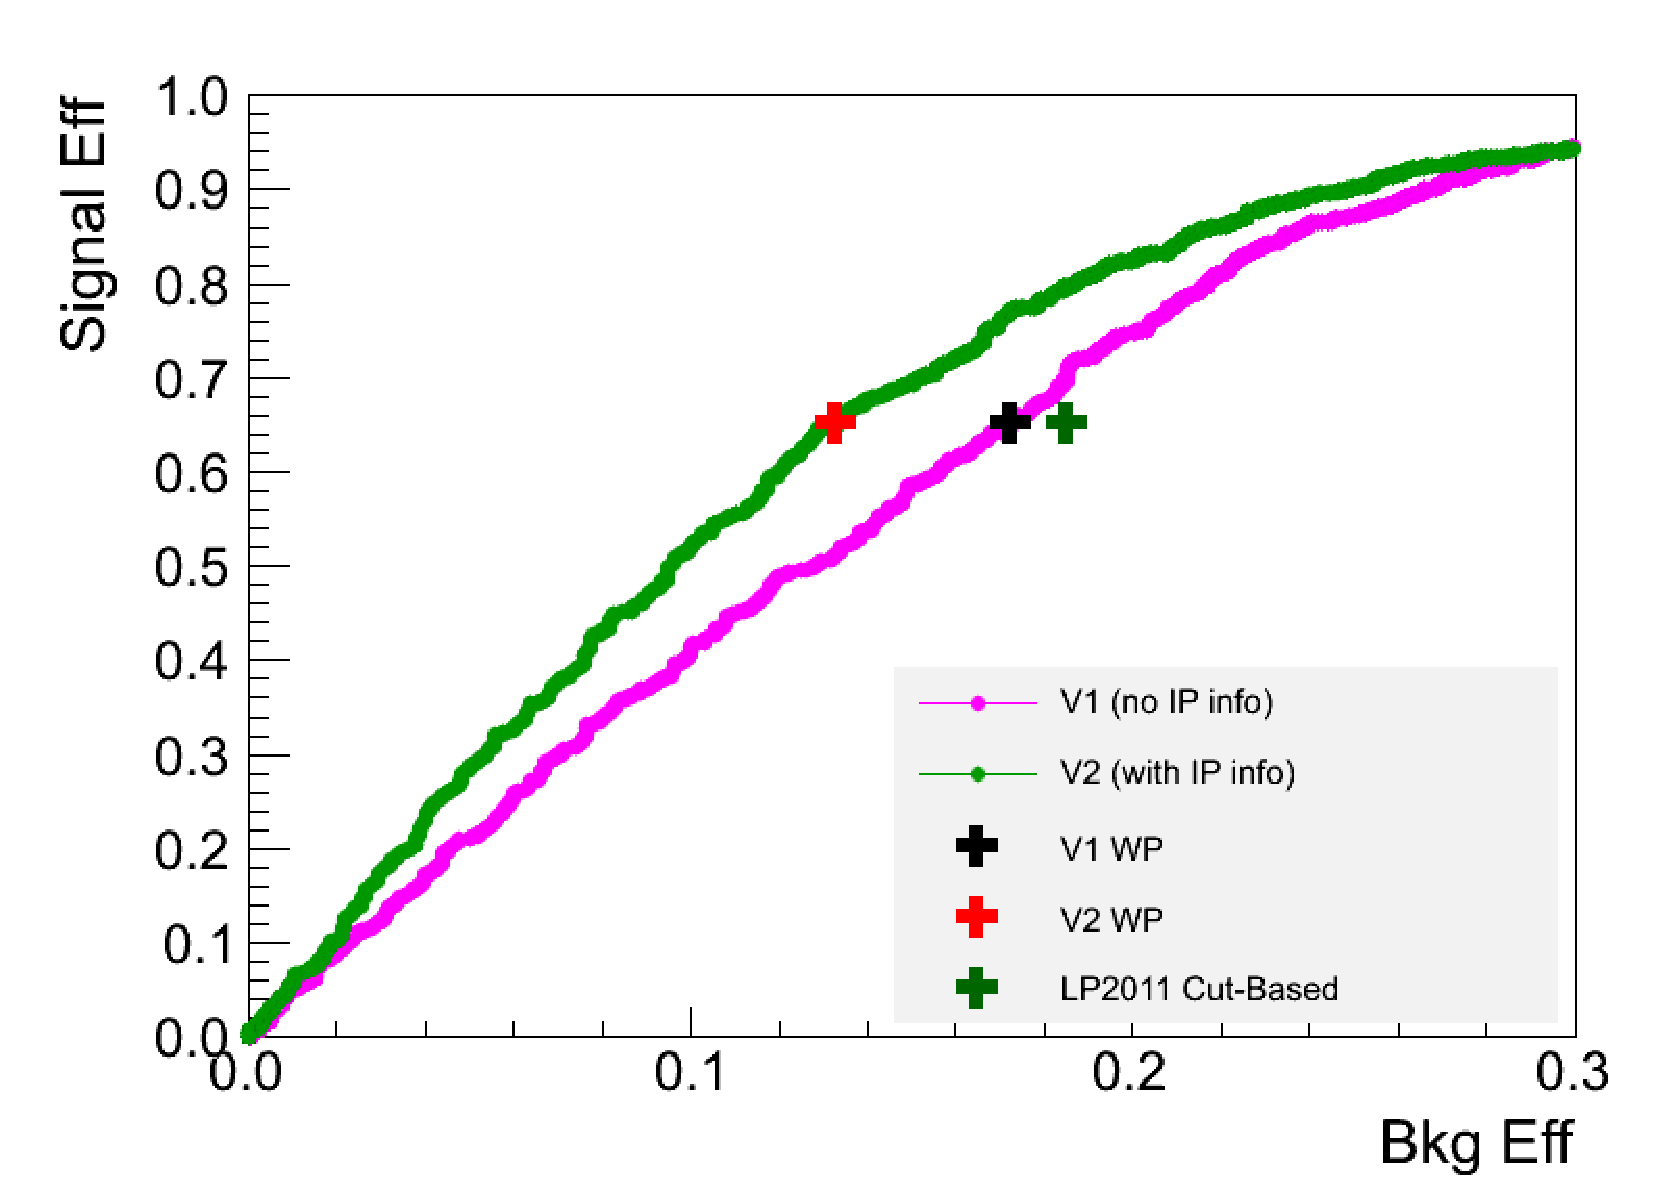
\includegraphics[width=0.45\textwidth]{figures/ROCGraphs_ElectronIDMVA_WithAndWithoutIPInfoSubdet1LowPt_HWW115.pdf}}
\subfigure[$10 \le \pt < 20$, $1.5 \le |\eta| < 2.5$]{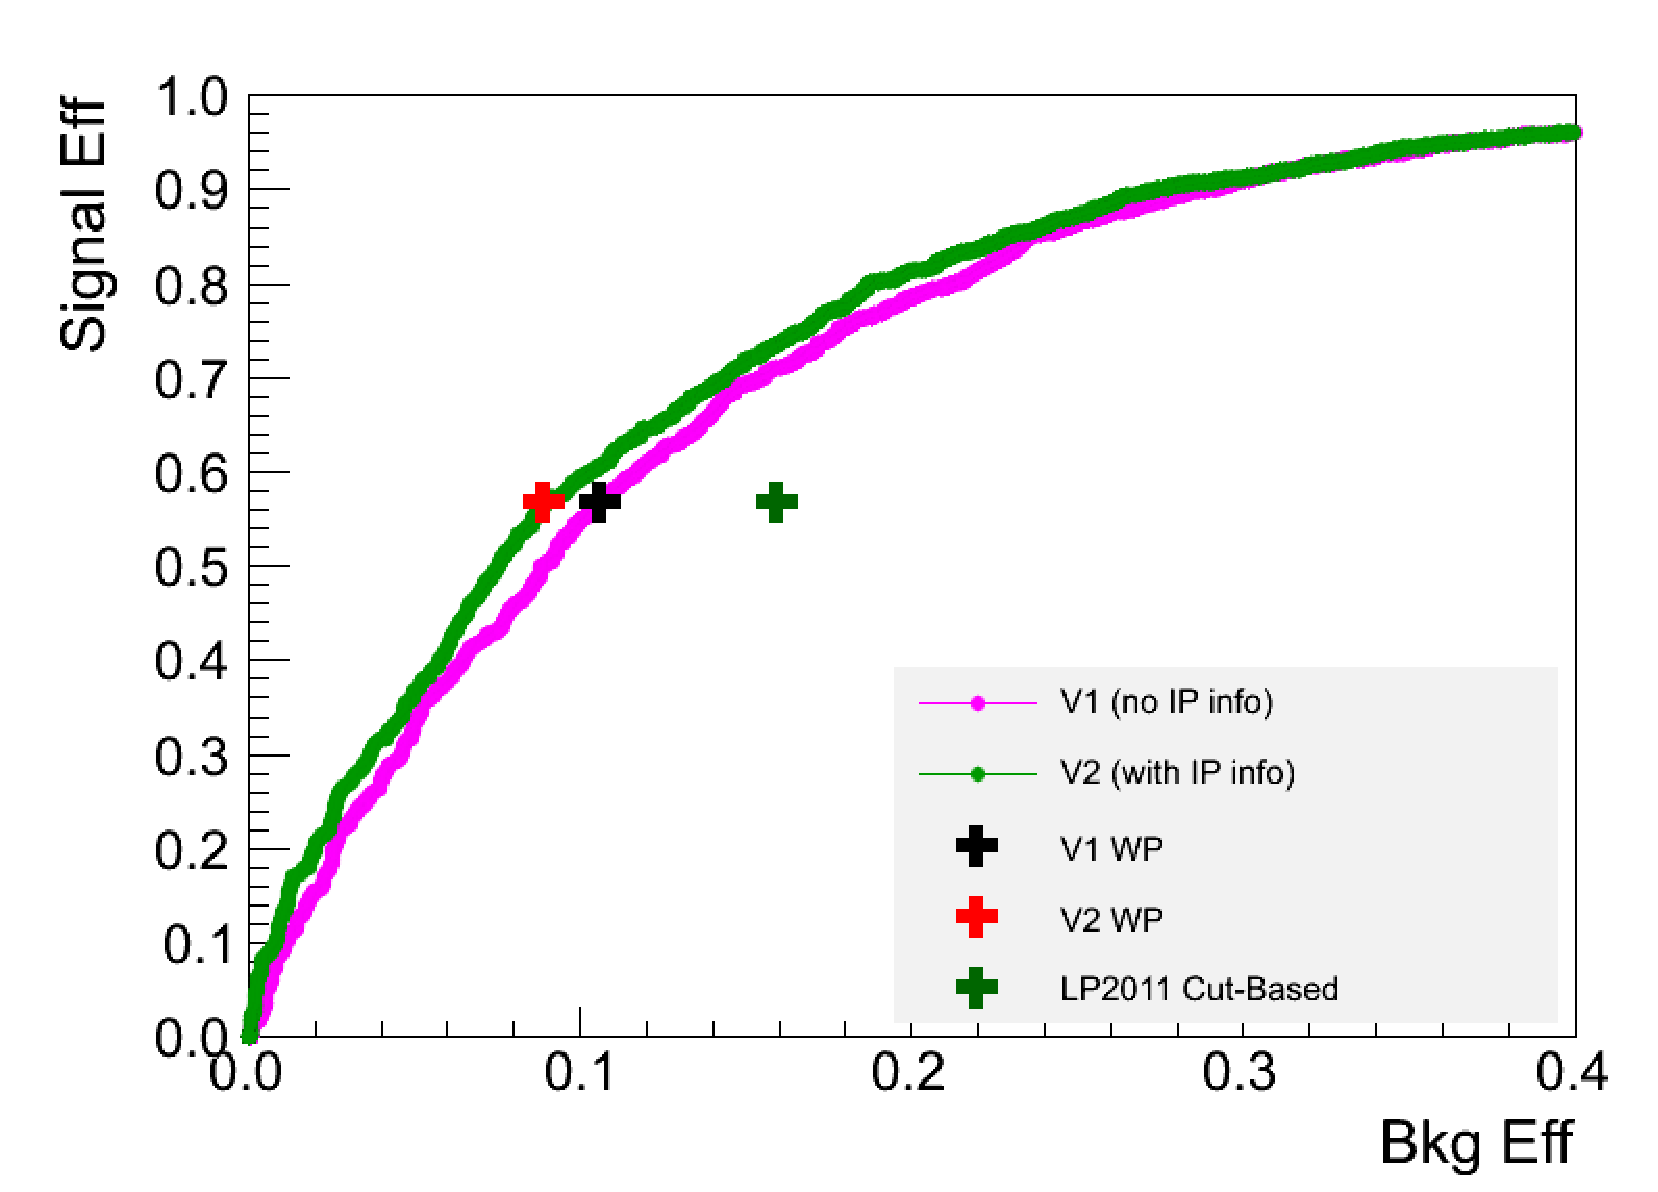
\includegraphics[width=0.45\textwidth]{figures/ROCGraphs_ElectronIDMVA_WithAndWithoutIPInfoSubdet2LowPt_HWW115.pdf}}
\subfigure[$\pt \ge 20$, $|\eta| < 1.0$]{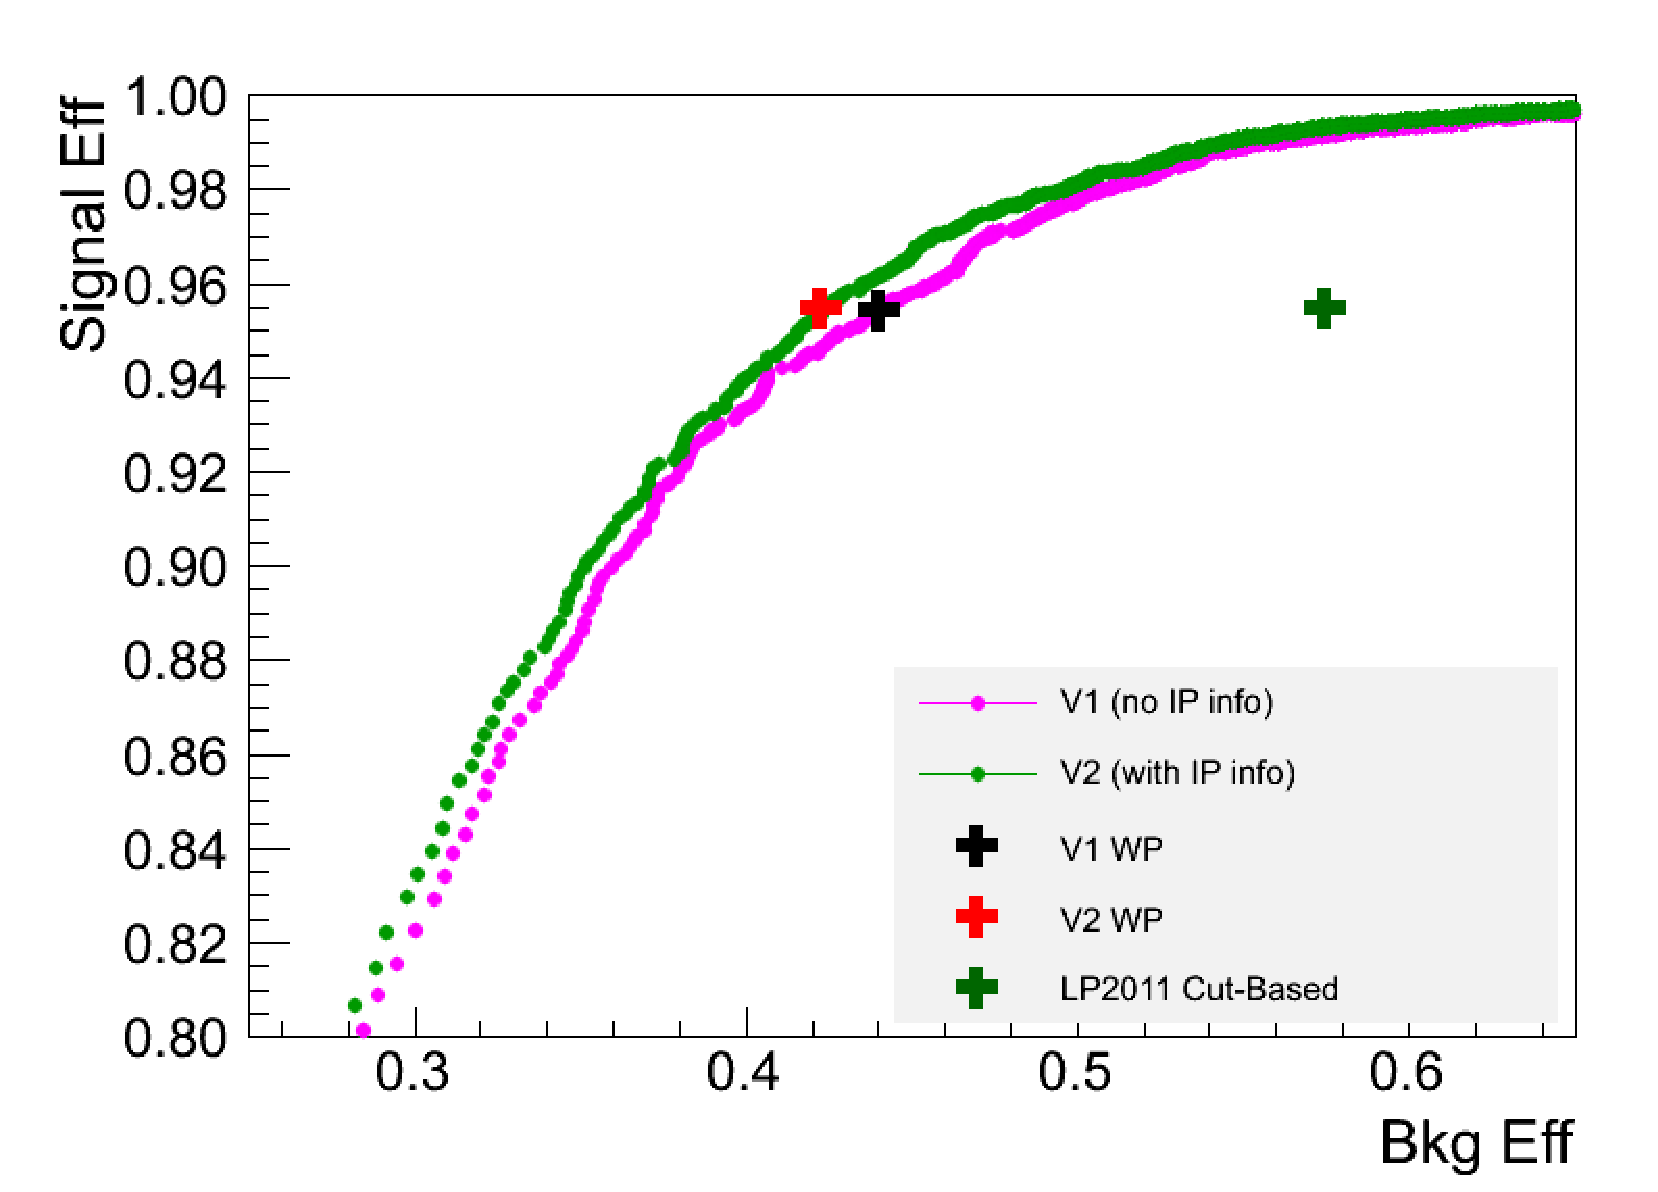
\includegraphics[width=0.45\textwidth]{figures/ROCGraphs_ElectronIDMVA_WithAndWithoutIPInfoSubdet0HighPt_HWW115.pdf}}
\subfigure[$\pt \ge 20$, $1.0 \le |\eta| < 1.5$]{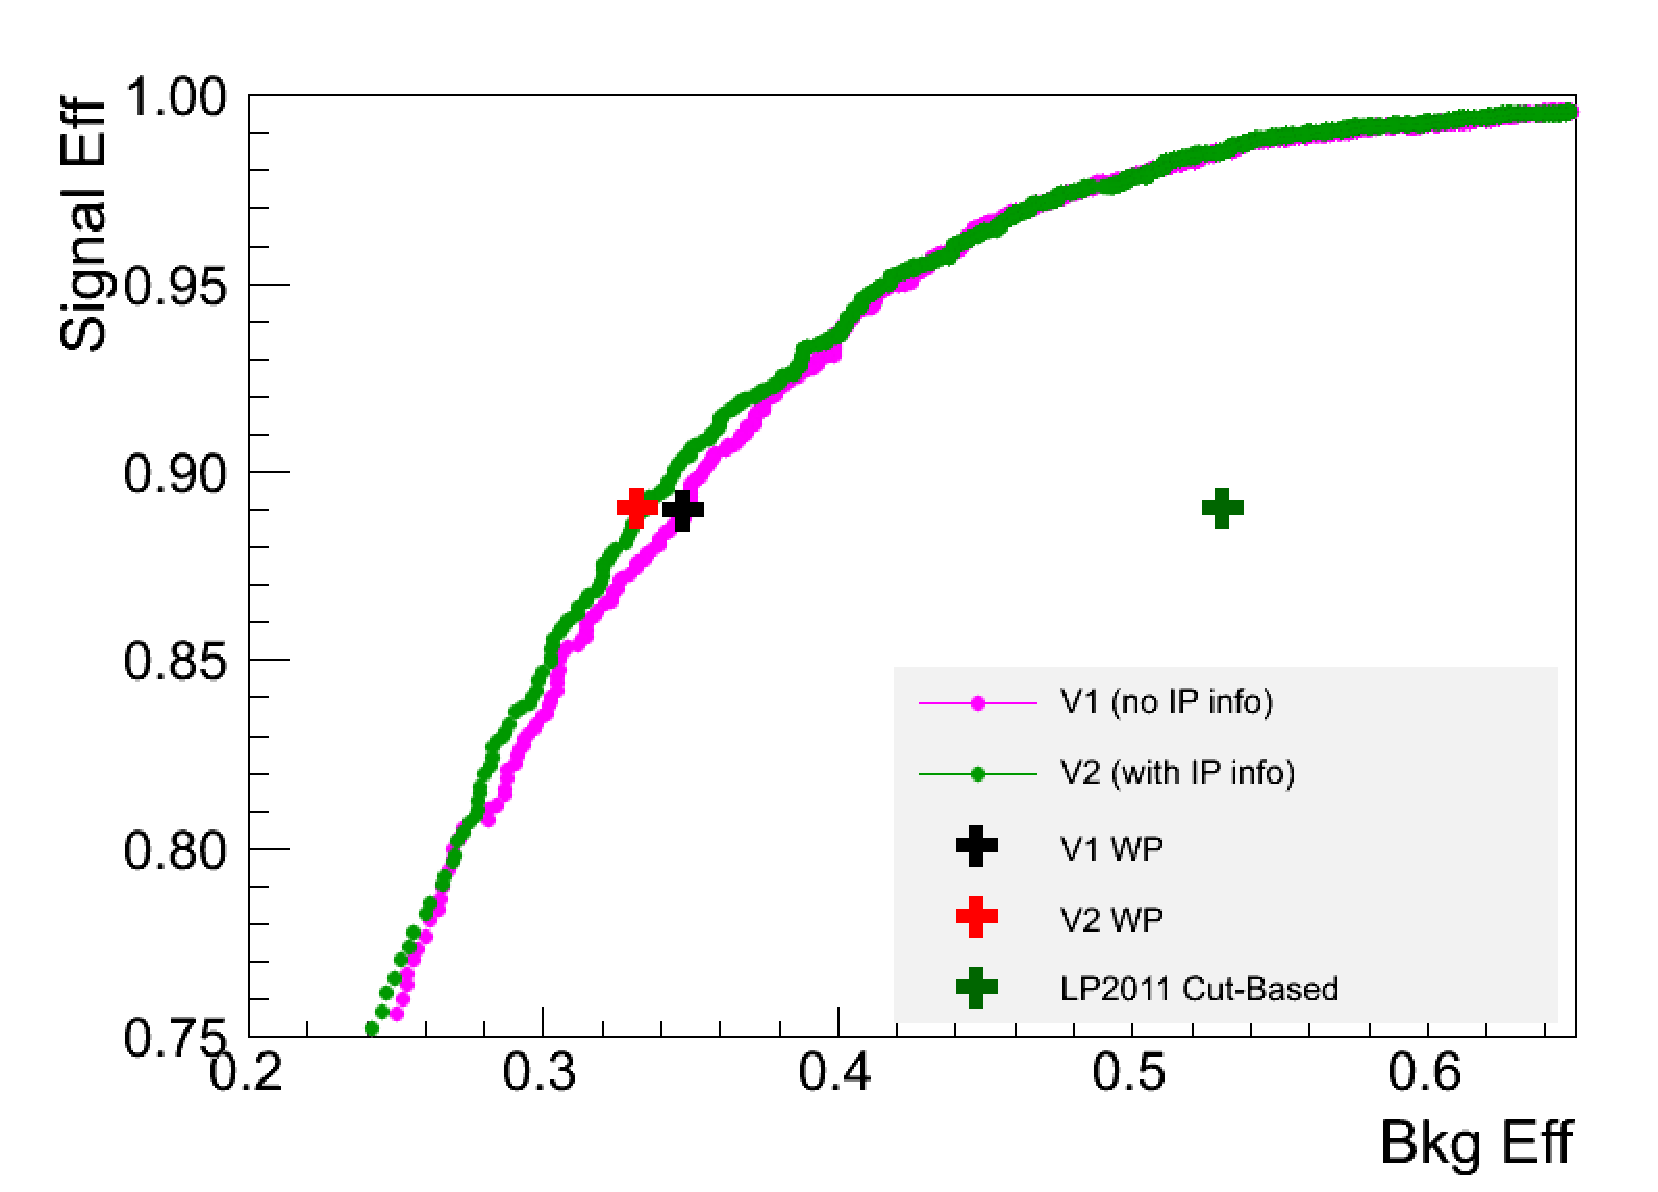
\includegraphics[width=0.45\textwidth]{figures/ROCGraphs_ElectronIDMVA_WithAndWithoutIPInfoSubdet1HighPt_HWW115.pdf}}
\subfigure[$\pt \ge 20$, $1.5 \le |\eta| < 2.5$]{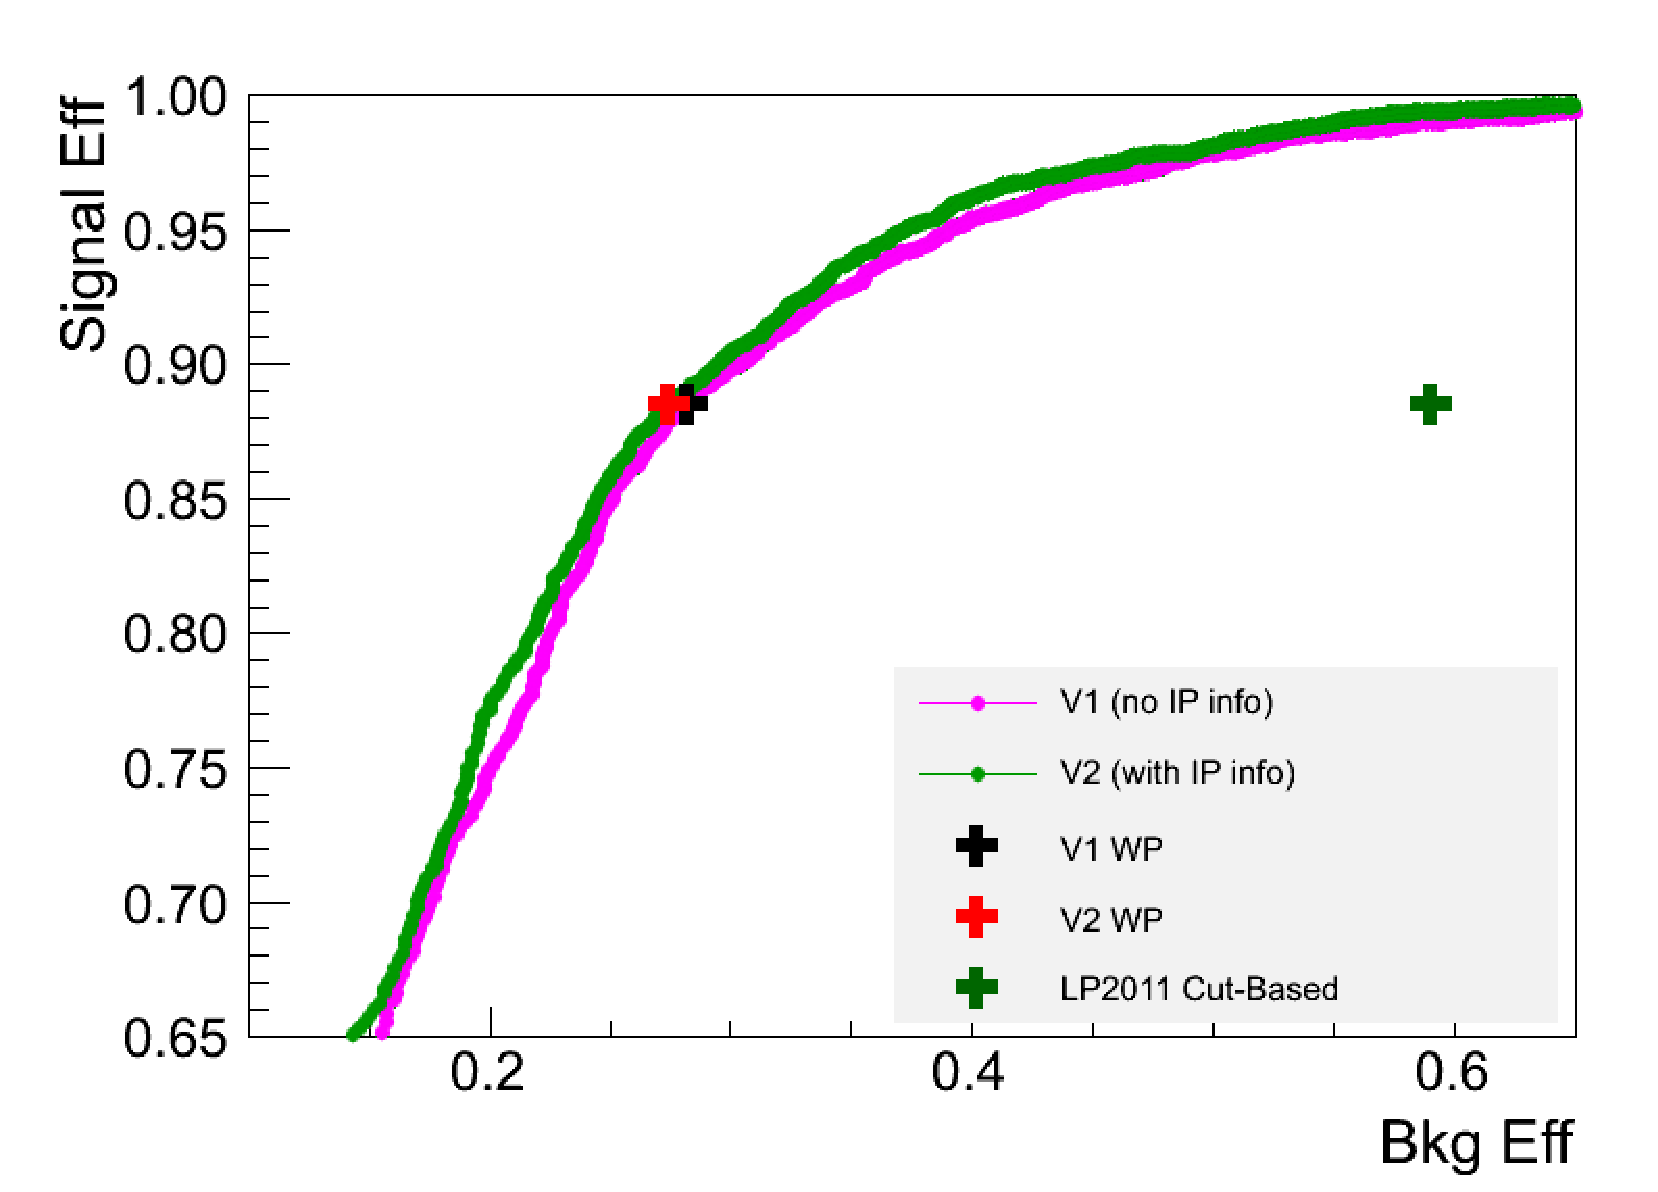
\includegraphics[width=0.45\textwidth]{figures/ROCGraphs_ElectronIDMVA_WithAndWithoutIPInfoSubdet2HighPt_HWW115.pdf}}
\caption{ROC curves for the BDT discriminator with and without the impact parameter
variables. The signal efficiency is computed from the \hww\ signal Monte Carlo
sample with a Higgs mass hypothesis of $115\GeV$. 
The working point used for the cut based electron selection is shown in the green cross.
The red and black crosses show the new proposed working points for the BDT discriminator 
with and without the impact parameter variables respectively.
}
\label{fig:ROC_Performance} 
\end{center}
\end{figure}
 
\section{Application to the \hww\ Analysis}
The newly defined working point for the BDT discriminator that includes the impact parameter variables is summarized in Table \ref{tab:BDTWithIPWorkingPoint}. We verify its performance gain by applying this electron selection for the \hww\ analysis. 

\begin{table}[!htbp]
\begin{center}
\begin{tabular}{|c|c|}
\hline
    Electron Bin                              &        BDT Cut Value  \\
 \hline
    $10 \le \pt < 20$, $|\eta| < 1.0$         &        BDT $> 0.139$  \\ 
 \hline
    $10 \le \pt < 20$, $1.0 \le |\eta| < 1.5$ &        BDT $> 0.525$  \\ 
 \hline
    $10 \le \pt < 20$, $1.5 \le |\eta| < 2.5$ &        BDT $> 0.543$  \\ 
 \hline
    $\pt \ge 20$, $|\eta| < 1.0$              &        BDT $> 0.947$  \\ 
 \hline
    $\pt \ge 20$, $1.0 \le |\eta| < 1.5$      &        BDT $> 0.950$  \\ 
 \hline
    $\pt \ge 20$, $1.5 \le |\eta| < 2.5$      &        BDT $> 0.884$  \\ 
 \hline
\end{tabular}
\caption{Cut values on the BDT output in each kinematic region for the newly defined working point using the BDT that includes impact parameter information. }
\label{tab:BDTWithIPWorkingPoint}
\end{center}
\end{table}


Fake rates extracted using the procedure defined in reference \cite{hww_eps}, are summarized numerically in Table \ref{tab:FakeRates}. They are compared with the fake rate for the cut based electron selection in Figure \ref{fig:FakeRates} as a function of \pt\ and $\eta$.


\begin{table}[!htbp]
\begin{center}
\begin{tabular}{|c|c|c|c|c|c|}
\hline
                       &        $0<\eta<0.5$      &        $1<\eta<1.5$      &        $1.5<\eta<2$      &        $2<\eta<2.5$       \\
 \hline
    $10 < p_{T} <= 15$ &        $0.060 +/- 0.009$ &        $0.041 +/- 0.009$ &        $0.018 +/- 0.006$ &        $0.032 +/- 0.010$  \\ 
 \hline
    $15 < p_{T} <= 20$ &        $0.072 +/- 0.009$ &        $0.045 +/- 0.009$ &        $0.015 +/- 0.005$ &        $0.041 +/- 0.009$  \\ 
 \hline
    $20 < p_{T} <= 25$ &        $0.082 +/- 0.009$ &        $0.051 +/- 0.009$ &        $0.050 +/- 0.008$ &        $0.044 +/- 0.008$  \\ 
 \hline
    $25 < p_{T} <= 30$ &        $0.070 +/- 0.009$ &        $0.052 +/- 0.010$ &        $0.036 +/- 0.008$ &        $0.058 +/- 0.010$  \\ 
 \hline
    $30 < p_{T} <= 35$ &        $0.074 +/- 0.011$ &        $0.089 +/- 0.015$ &        $0.074 +/- 0.012$ &        $0.054 +/- 0.011$  \\ 
 \hline
\end{tabular}
\caption{Electron fake rate in $\eta$-$p_T$ using data from the Lepton Photon 2011 dataset. 
Uncertainties are statistical only. A combination of the {\bf Ele8\_CaloIdL\_CaloIsoVL}, {\bf Ele17\_CaloIdL\_CaloIsoVL}, 
{\bf Ele8\_CaloIdL\_CaloIsoVL\_Jet40} triggers are used, with a $p_{T}$ threshold on the leading jet in
the event of $35$ GeV. }
\label{tab:FakeRates}
\end{center}
\end{table}

\begin{figure}[!htbp]
\begin{center}
\subfigure[Fake rates as a function of \pt]{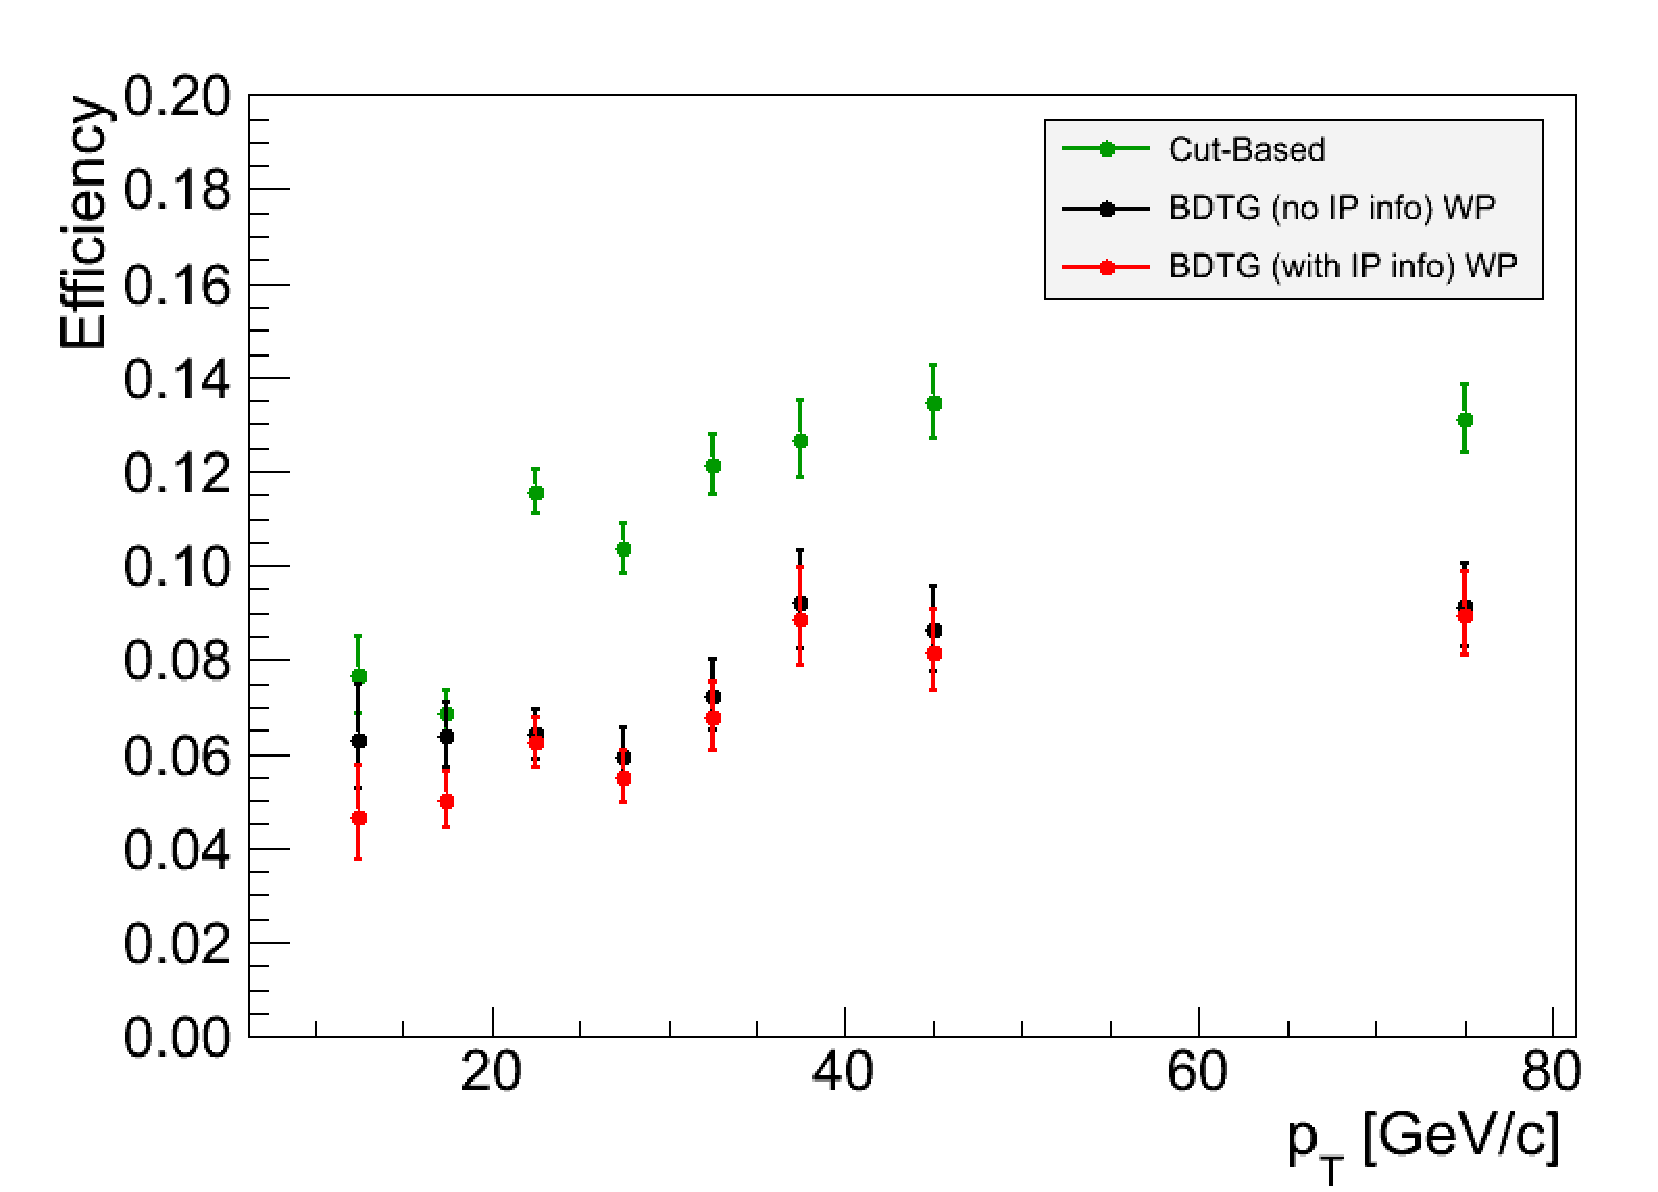
\includegraphics[width=0.45\textwidth]{figures/ElectronFakeRate_CutBasedVsMVA_Pt.pdf}}
\subfigure[Fake rates as a function of $\eta$]{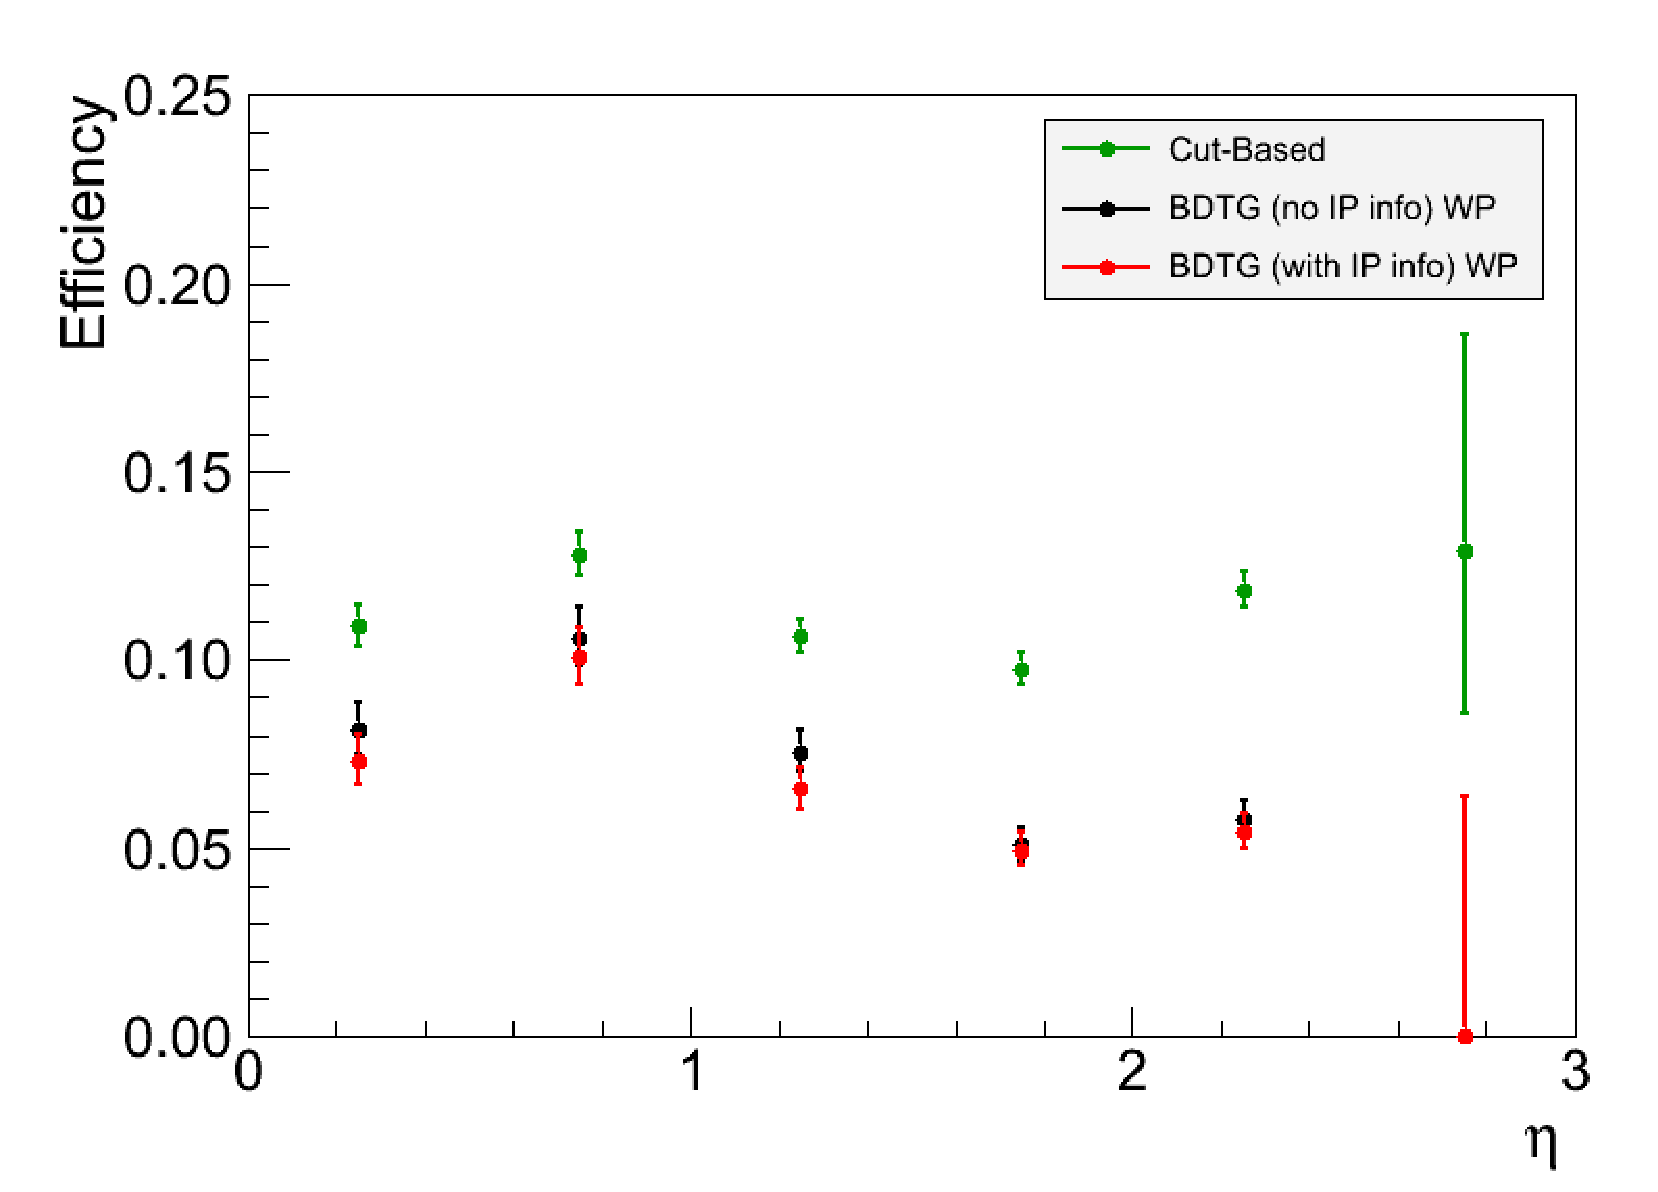
\includegraphics[width=0.45\textwidth]{figures/ElectronFakeRate_CutBasedVsMVA_Eta.pdf}}
\caption{Fake rates as a function of \pt\ and $\eta$ for the cut based electron selection and the two BDT selections.}
\label{fig:FakeRates}
\end{center}
\end{figure}

We also measure the data to Monte Carlo efficiency scale factors for the new working point. The results are summarized in Table \ref{tab:EfficiencyScaleFactors}, and show that the Monte Carlo to data corrections are small. This fact is also evident from Figure \ref{fig:BDT_Distributions} which show the comparison of the BDT discriminator distribution between data and signal Monte Carlo.

\begin{table}[!ht]
\begin{center}
\begin{tabular}{|c|c|c|c|}
\hline
Bin                                        & Monte Carlo Efficiency & Data Efficiency     & Scale Factor           \\ 
\hline
$10 \le \pt < 15$, $0 \le |\eta| < 1.479$    & 0.417 $\pm$ 0.004      & 0.418 $\pm$ 0.002   & 1.003 $\pm$ 0.011    \\ 
$10 \le \pt < 15$, $1.479 \le |\eta| < 2.5$  & 0.193 $\pm$ 0.003      & 0.204 $\pm$ 0.010   & 1.054 $\pm$ 0.055    \\ 
$15 \le \pt < 20$, $0 \le |\eta| < 1.479$    & 0.556 $\pm$ 0.003      & 0.536 $\pm$ 0.003   & 0.965 $\pm$ 0.006    \\ 
$15 \le \pt < 20$, $1.479 \le |\eta| < 2.5$  & 0.301 $\pm$ 0.003      & 0.299 $\pm$ 0.007   & 0.993 $\pm$ 0.026    \\ 
$20 \le \pt $, $0 \le |\eta| < 1.479$        & 0.8384 $\pm$ 0.0003    & 0.8262 $\pm$ 0.0007 & 0.9854 $\pm$ 0.0009  \\ 
$20 \le \pt $, $1.479 \le |\eta| < 2.5$      & 0.6565 $\pm$ 0.0006    & 0.6673 $\pm$ 0.0006 & 1.0164 $\pm$ 0.0009  \\ 
\hline
\end{tabular}
\caption{Data to Monte Carlo efficiency scale factors for the new BDT working point.}
\label{tab:EfficiencyScaleFactors}
\end{center}
\end{table}

\begin{figure}[!htbp]
\begin{center}
\subfigure[$10 \le \pt < 20$, $|\eta| < 1.0$]{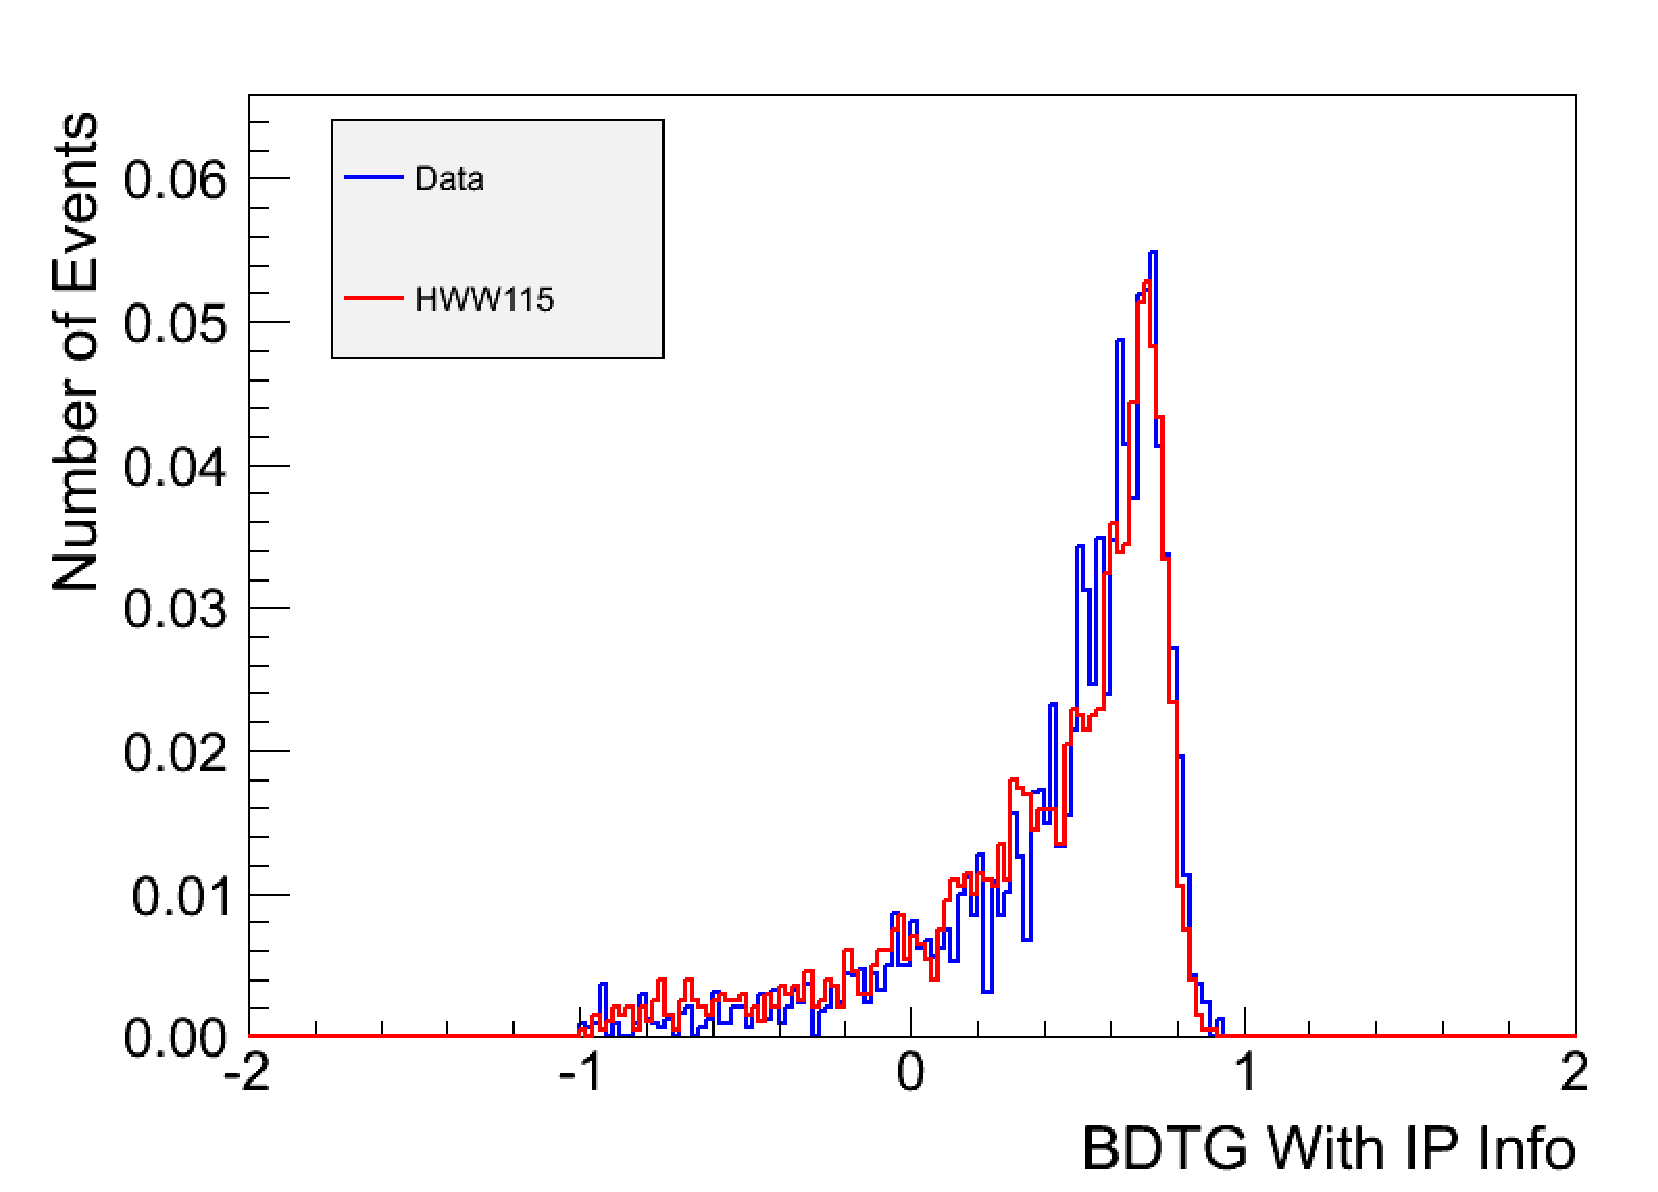
\includegraphics[width=0.45\textwidth]{figures/EleBDTGV2_Subdet0LowPt_Real.pdf}}
\subfigure[$10 \le \pt < 20$, $1.0 \le |\eta| < 1.5$]{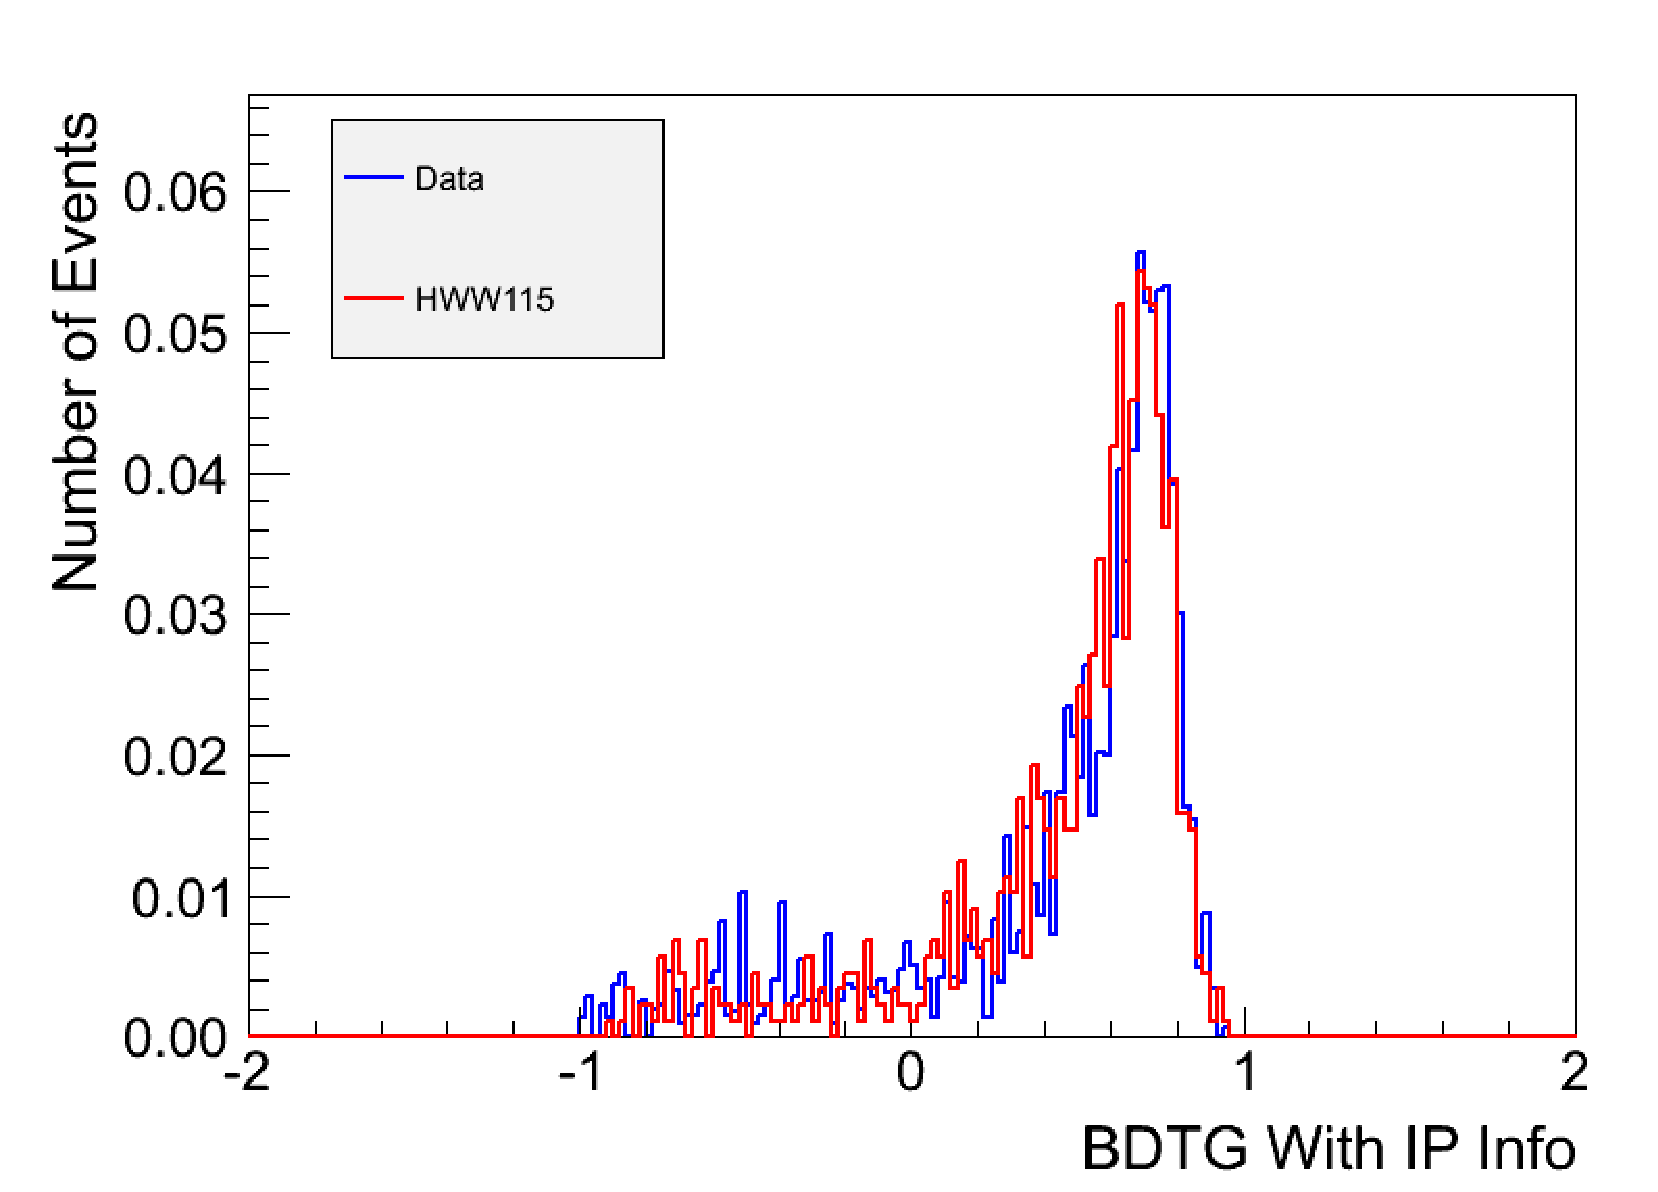
\includegraphics[width=0.45\textwidth]{figures/EleBDTGV2_Subdet1LowPt_Real.pdf}}
\subfigure[$10 \le \pt < 20$, $1.5 \le |\eta| < 2.5$]{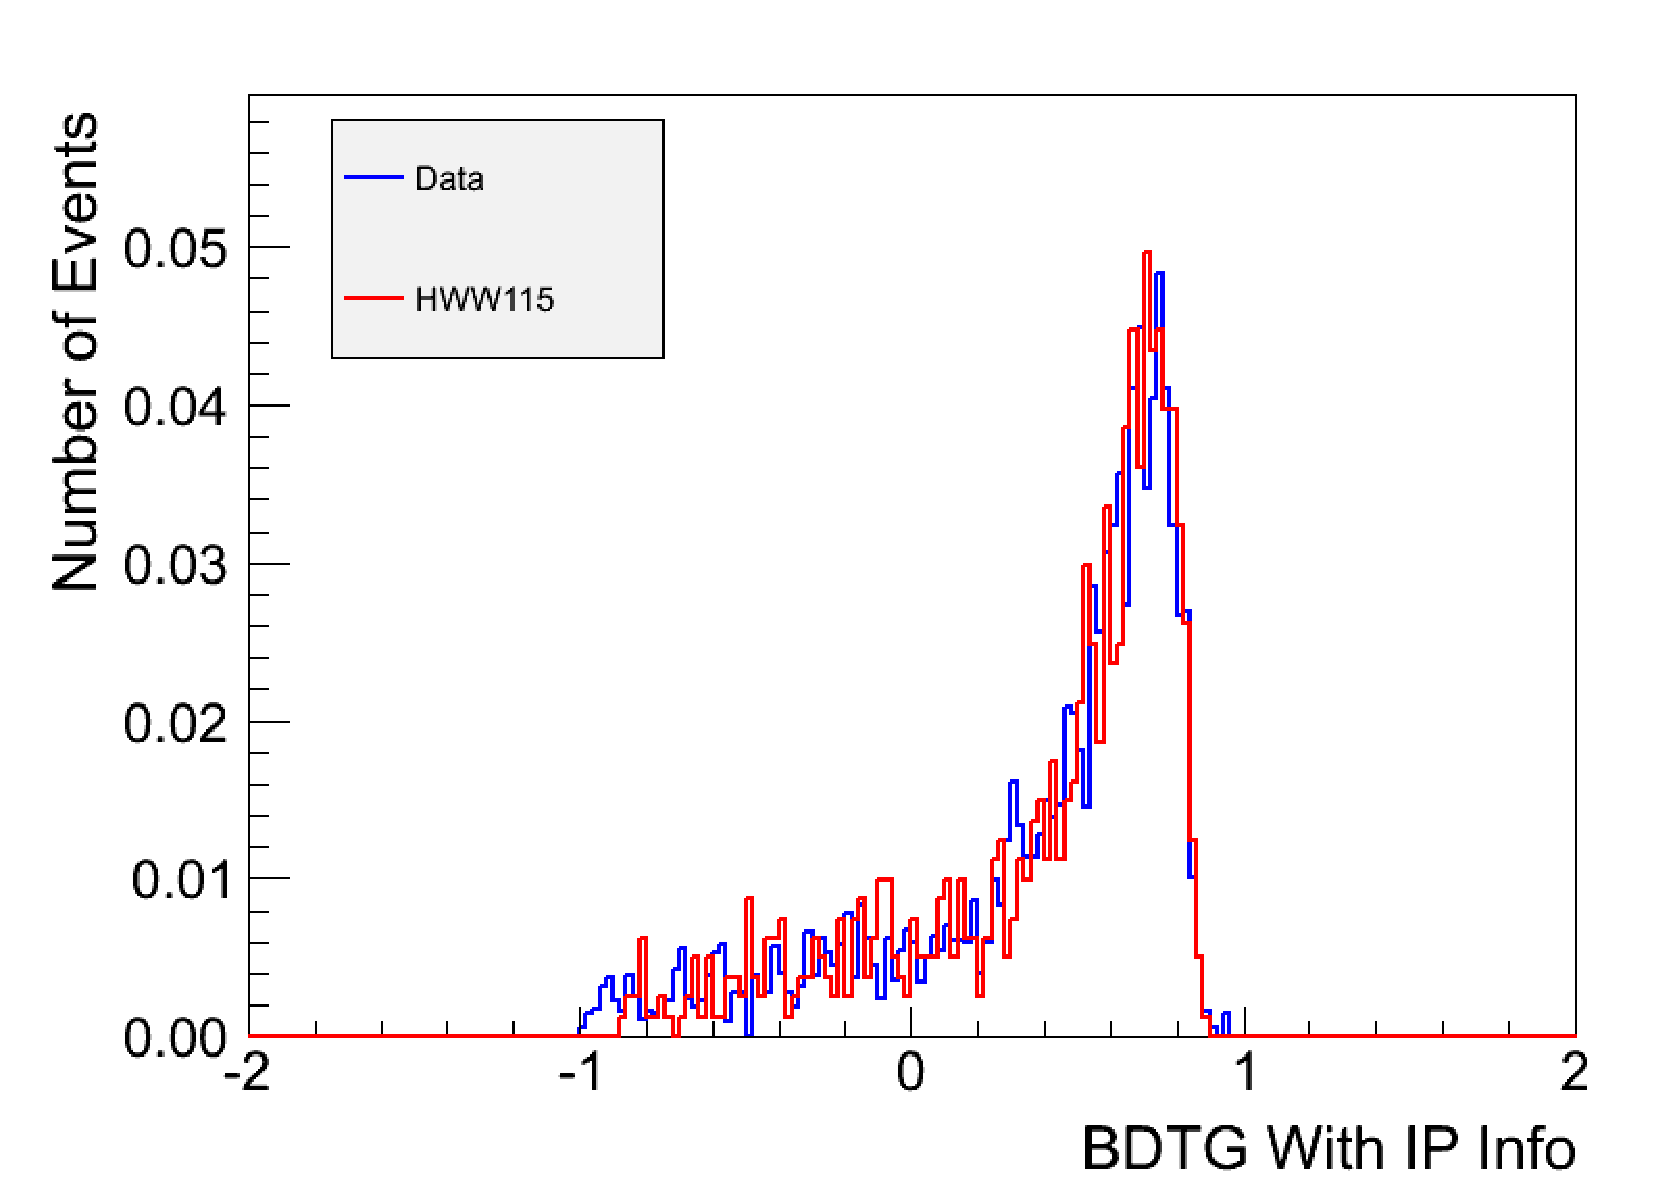
\includegraphics[width=0.45\textwidth]{figures/EleBDTGV2_Subdet2LowPt_Real.pdf}}
\subfigure[$\pt \ge 20$, $|\eta| < 1.0$]{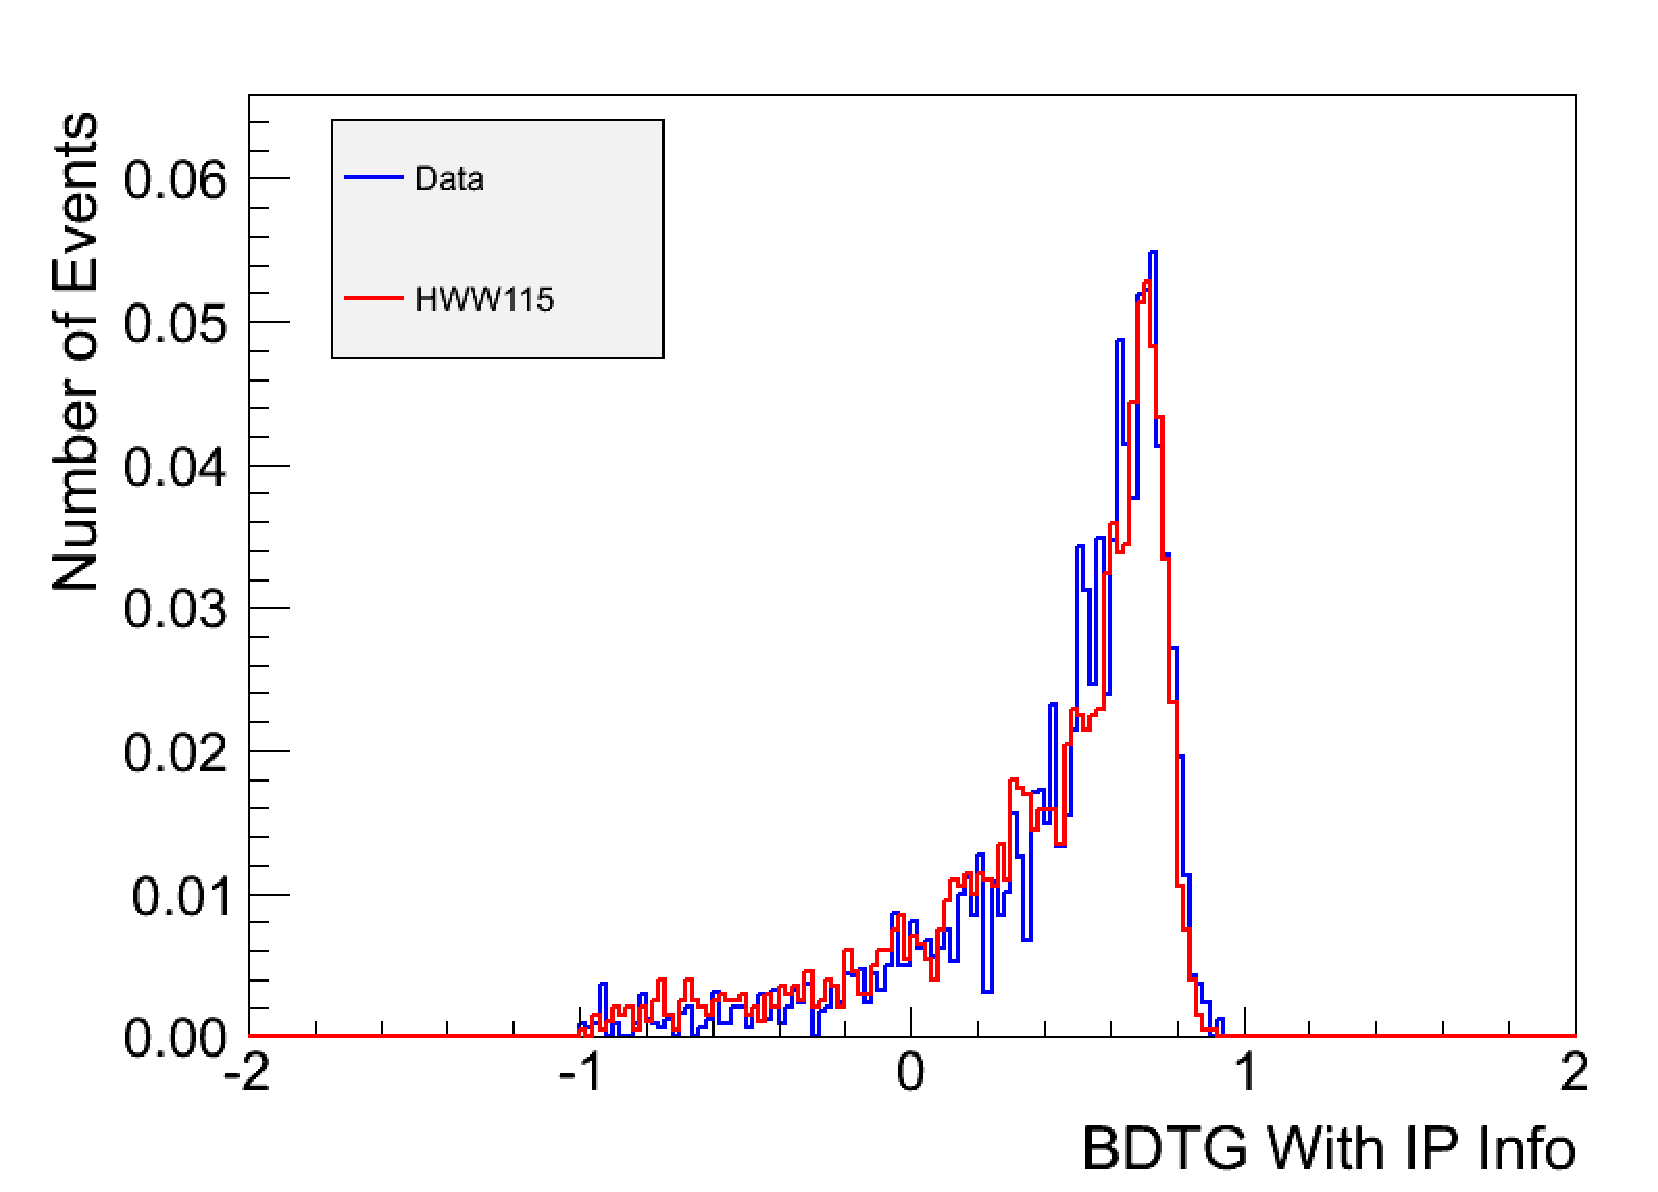
\includegraphics[width=0.45\textwidth]{figures/EleBDTGV2_Subdet0LowPt_Real.pdf}}
\subfigure[$\pt \ge 20$, $1.0 \le |\eta| < 1.5$]{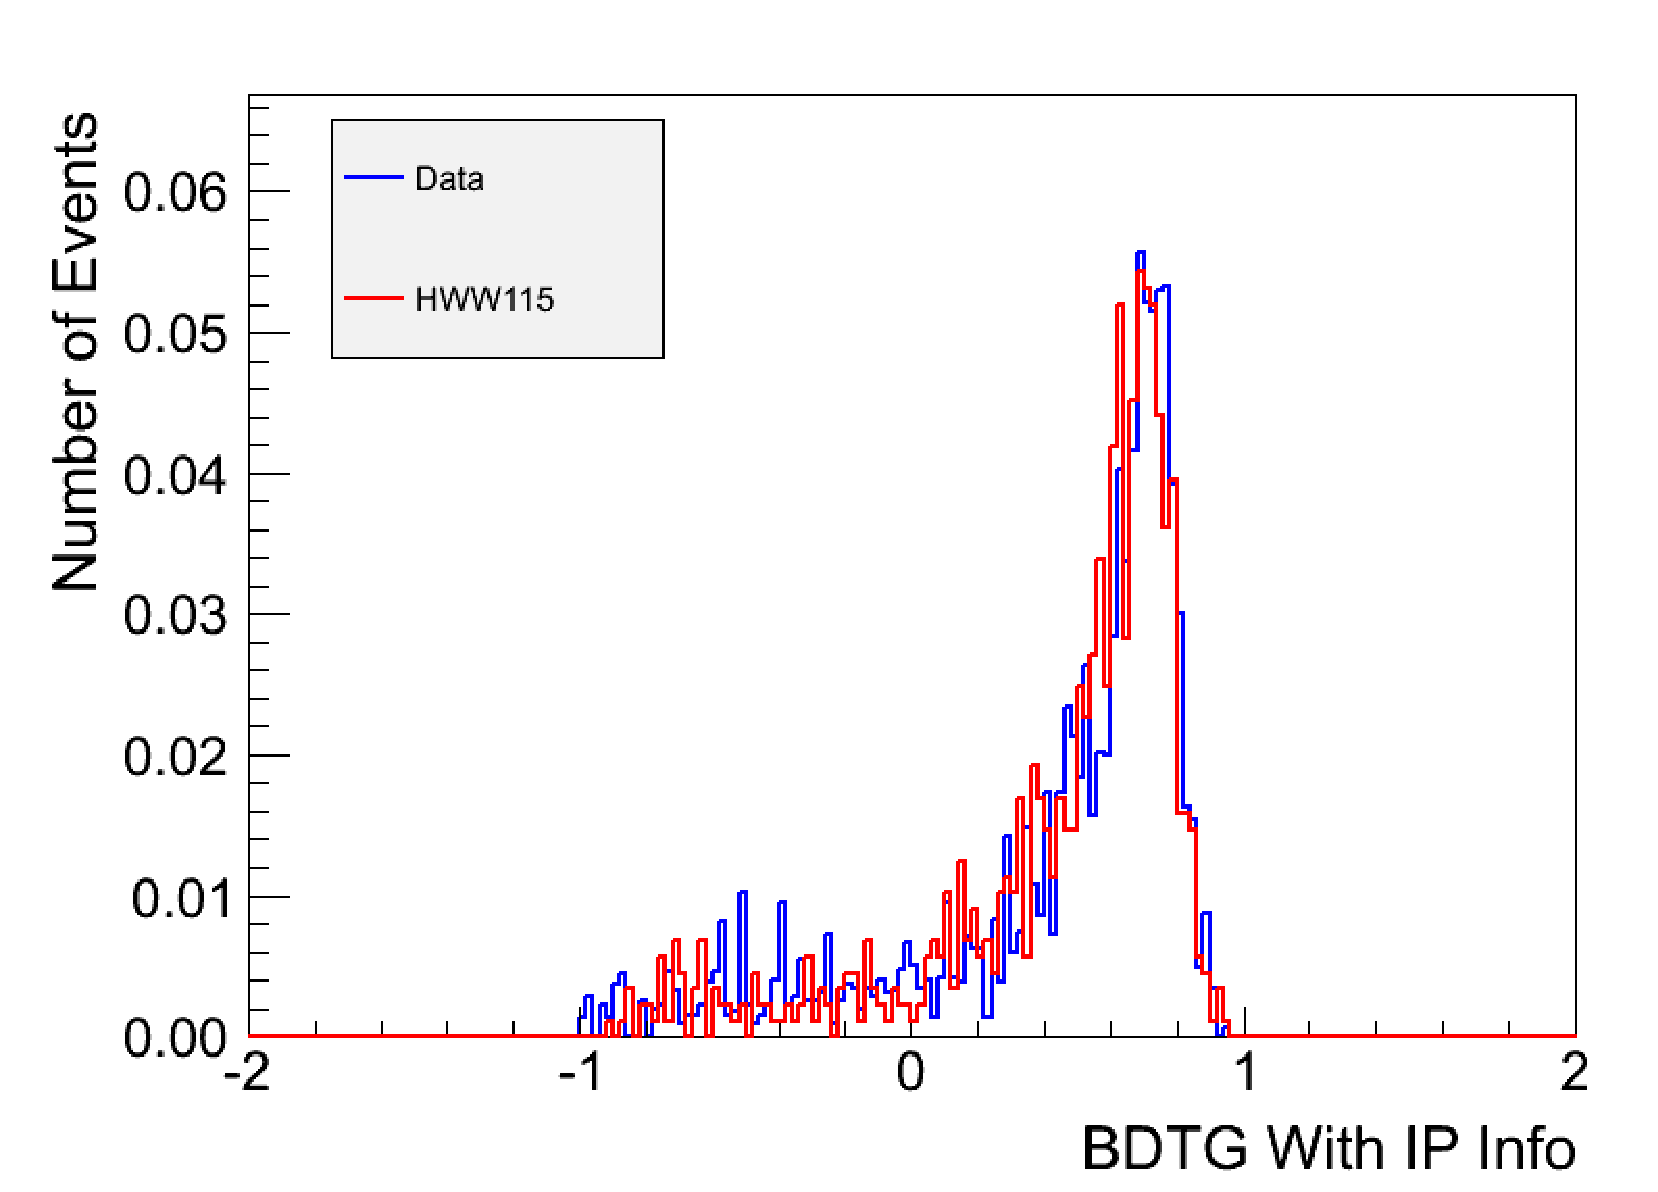
\includegraphics[width=0.45\textwidth]{figures/EleBDTGV2_Subdet1LowPt_Real.pdf}}
\subfigure[$\pt \ge 20$, $1.5 \le |\eta| < 2.5$]{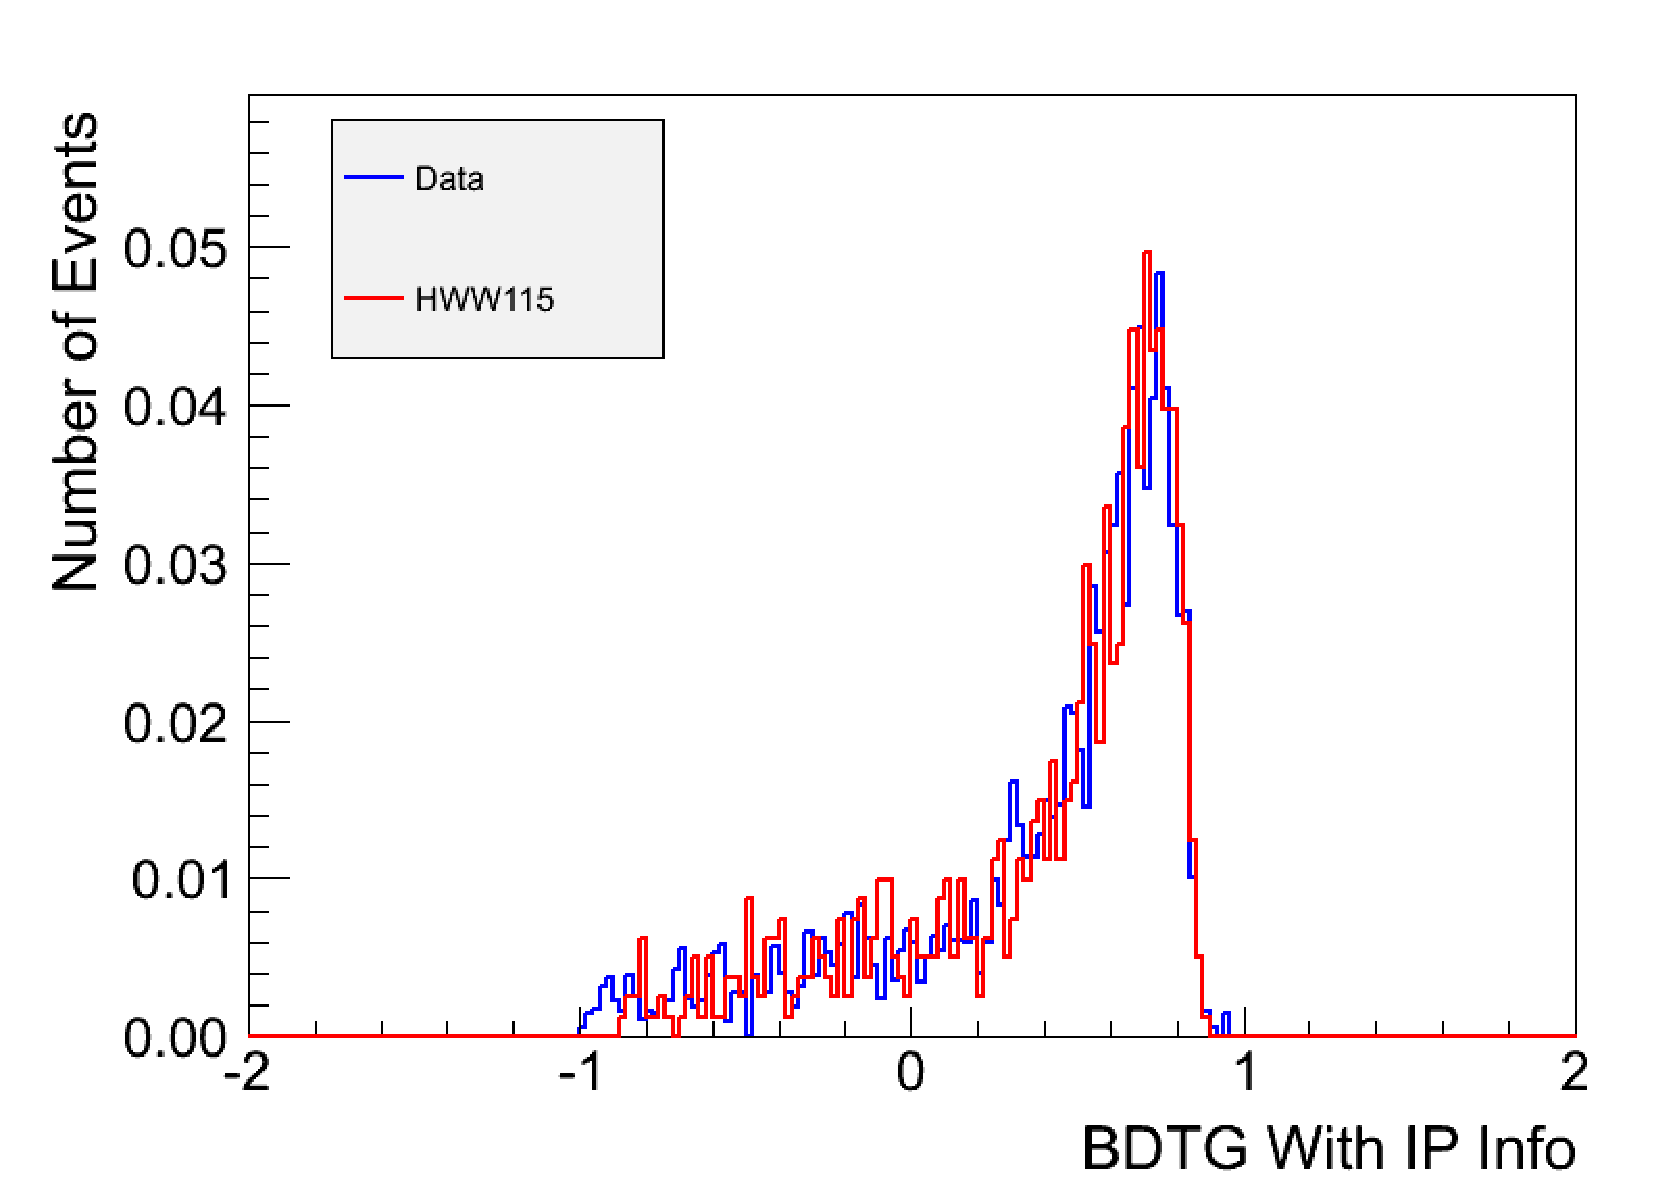
\includegraphics[width=0.45\textwidth]{figures/EleBDTGV2_Subdet2LowPt_Real.pdf}}
\caption{A comparison of the BDT discriminator distribution between data and signal Monte Carlo, separately for electrons in each of the six $\pt$ and $\eta$ bins.
}
\label{fig:BDT_Distributions} 
\end{center}
\end{figure}


Using the efficiency and fake rate measurements above we perform the full \hww\ analysis for the $120$\GeV\ mass hypothesis. The yields for the signal and the W+jets background the $m_{\mathrm{H}} = 120$\GeV\ analysis are shown in Table \ref{tab:HWW120Yield} for the cut based selection and the BDT selection. We see that for roughly the same signal yield, we reduce the fake electron background by $45\%$ and the total W+jets background by $25\%$. 


\begin{table}[!ht]
\begin{center}
\begin{tabular}{|c|c|c|}
\hline
\multicolumn{3}{|c|}{ 0 Jet Bin }               \\ 
\hline
Process                                      & Yields using cut based electron selection & Yields using BDT electron selection \\ 
\hline
W+Jets           & 31.6 (16.3)     & 23.8 (9.0) \\ 
HWW 120 Signal   & 11.7            & 11.4       \\ 
\hline
\multicolumn{3}{|c|}{ 1 Jet Bin }               \\ 
\hline
Process                                      & Yields using cut based electron selection & Yields using BDT electron selection \\ 
\hline
W+Jets           & 9.7 (4.4)       & 8.1 (2.5)  \\ 
HWW 120 Signal   & 4.1             & 3.8        \\ 
\hline
\multicolumn{3}{|c|}{ 2 Jet Bin }               \\ 
\hline
Process                                      & Yields using cut based electron selection & Yields using BDT electron selection \\ 
\hline
W+Jets           & 0.9             & 0.6        \\ 
HWW 120 Signal   & 0.6             & 0.6        \\ 
\hline
\end{tabular}
\caption{Data to Monte Carlo efficiency scale factors for the new BDT working point.}
\label{tab:HWW120Yield}
\end{center}
\end{table}


\section{Future Improvements}

A number of additional observables may be added to the BDT to further increase signal to background discrimination. One of the important variables that has not been used is the hadronic to electromagnetic energy ratio (H/E) due to its sensitivity to pileup. Future modifications of the exact algorithm used to compute this observable should render it insensitive to pileup, and therefore should give additional discrimination between electrons and charged pions and kaons. Use of the measured electron charge in combination with shower shape variables or $\Delta \phi_{\mathrm{in}}$ can give added discriminatory power as background and signal behave differently with respect to them. 

Use of the preshower detector could give additional discrimination between conversion electrons from neutral pion decays and prompt electrons. The matching in $\eta$ and $\phi$ between the cluster position and the electron track extrapolated to the calorimeter may give additional performance gains, as well as the $\chi^{2}$/degree of freedom for the electron GSF track. Additional shower shape information in the form of the $\eta$-width and $\phi$-width of the supercluster can also give additional discrimination power. Finally, adding single crystal information to the MVA in order to allow it to make use of the correlations can yield gains in performance. However, the inclusion of additional information may require larger training samples in order for the multivariate methods to properly make use of them.

Another outstanding question that is left unanswered is whether the performance can be improved with larger training samples. This can be tested in the future by varying the size of the training sample and observing whether there are significant changes in performance. 

\section{Conclusions}
  \label{sec:summary}
We have implemented a multivariate approach to electron identification using a boosted decision tree and studied the performance gain over the simple cut based approach. We observe an improvement of roughly $40\%$ to $50\%$ in the background rejection at the same signal efficiency as the cut based working point used for the \hww\ analysis. Fake rates and signal efficiency measurements were made verifying that the Monte Carlo simulation description of the BDT discriminator is reasonably accurate. The application of this BDT based electron selection on the \hww\ analysis with a signal mass hypothesis of $120$ \GeV\ shows that one can reduce the fake electron background by $45\%$ and the total W+Jets background by about $25\%$.



%===================================================================================================
\clearpage

\vspace*{-0.2cm}
\thebibliography{12}

\bibitem{pdg}
 K. Nakamura et al. (Particle Data Group), "Review of particle physics", J. Phys.G37 , 2010.

\bibitem{Higgs1}
F. Englert and R. Brout, "Broken symmetries and the masses of gauge bosons", Phys. Rev. Lett. 13,  1964.

\bibitem{Higgs2}
P. W. Higgs, "Broken symmetry and the mass of gauge vector mesons", Phys. Rev. Lett. 13, 1964.

\bibitem{Higgs3}
Guralnik, G.S. and Hagen, C.R. and Kibble, T.W.B., "Global Conservation Laws and Massless Particles", 
Phys.Rev.Lett. 13, 1964.

\bibitem{dittmar}
M.~Dittmar and H.~K.~Dreiner, Phys.\ Rev.\  D {\bf 55} (1997) 167".

\bibitem{HWW2010}
CMS Collaboration, "Measurement of WW Production and Search for the Higgs Boson in 
pp Collisions at $\sqrt{s}$ = 7 TeV", arXiv:1102.5429

\bibitem{HWW2011AN}
L.~Bauerdick et al, "A Higgs Boson Search in the Fully Leptonic $W^+W^-$ Final State", CMS AN-2011/155

\bibitem{VBTFCrossSectionNote}
J. Alcaraz Maestre, \textit{et al.}, "Updated Measurements of Inclusive W and Z Cross Sections 
at $\sqrt{s}=7$ TeV", CMS AN-2010/264.

\bibitem{ggWWError}
F.~ Stoeckli, "http://indico.cern.ch/getFile.py/access?contribId=0\&resId=1\&materialId=slides\&confId=49009", 
EWK Diboson meeting of March 12 2009.

\bibitem{json}
{\small
/afs/cern.ch/cms/CAF/CMSCOMM/COMM\_DQM/certification/Collisions11/7TeV/Prompt/Cert\_160404-163869\_7TeV\_PromptReco\_Collisions11\_JSON.txt
}

\bibitem{ElIso}
A. Vartak, M. LeBourgeois, V. Sharma, "Lepton Isolation in the CMS Tracker, ECAL and HCAL", CMS AN-2010/106.

\bibitem{PVDA}
W. Erdmann, M. LeBourgeois, B. Mangano, 
https://indico.cern.ch/getFile.py/access?contribId=5\&sessionId=3\&resId=1\&materialId=slides\&confId=127127, 
note in preparation.

\bibitem{NExpHits}
B. Mangano \textit{et al.}, "Improvement in Photon Conversion Rejection Performance Using 
Advanced Tracking Tools", AN-10-283.

\bibitem{fakeLeptonNote1}
S.~Xie, \textit{et al.}", "Study of Data-Driven Methods for Estimation of Fake Lepton Backgrounds", 
CMS AN-2009/120.

\bibitem{fakeLeptonNote2}
W.~Andrews, \textit{et al.}, "Fake Rates for dilepton Analyses", CMS AN-2010/257.

\bibitem{fakeLeptonBkgSpillage1}
 F. Golf, D. Evans, J. Mulmenstadt  \textit{et al.}, ``Expectations for observation of top quark pair production in the dilepton final state with the early CMS data'', CMS AN-2009/050.

\bibitem{dyestnote}
W. Andrews, et al., “A Method to Measure the Contribution of $\dyll$ to a di-lepton+ MET Selection”, CMS AN-2009/023 (2009).

\bibitem{jes}
CMS Collaboration, "Jet Energy Calibration with Photon+Jet Events", PAS JME-09-004.

\bibitem{jetpas}
CMS Collaboration, "Jet Performance in pp Collisions at $\sqrt{s}=7 \rm\ TeV$", PAS JME-10-003.

\bibitem{btag}
CMS collaboration, "Commissioning of b-jet identification with pp collisions at $\sqrt{s}=7~\TeV$, BTV-10-001.

\bibitem{antikt}
Cacciari, Matteo and Salam, Gavin P. and Soyez, Gregory, "The anti-$k_t$ jet clustering 
algorithm", JHEP 04,  2008.

\bibitem{ConversionNote}
W.~Andrews, \textit{et al.}, "Study of photon conversion rejection at CMS", CMS AN-2009/159.

\bibitem{tmva}
A. Hoecker, \textit{et al.}, "TMVA - Toolkit for Multivariate Data Analysis", arXiv:physics/0703039, 2007.

\bibitem{XS}
CMS Generator group, Standard Model Cross Sections for CMS at 7 TeV, 2010.

\bibitem{PDF4LHC}
PDF4LHC Working Group, 
{\tt http://www.hep.ucl.ac.uk/pdf4lhc/PDF4LHCrecom.pdf}

\bibitem{Nadolsky:2008zw}
Nadolsky, Pavel M. and others, "Implications of CTEQ global analysis for 
collider observables", Phys. Rev. D78 2008.

\bibitem{Martin:2009iq}
Martin, A. D. and Stirling, W. J. and Thorne, R. S. and Watt, G., "Parton 
distributions for the LHC, Eur. Phys. J. C63 2009.

\bibitem{Ball:2010de}
Ball, Richard D. and others, "A first unbiased global NLO determination 
of parton distributions and their uncertainties", arXiv 1002.4407.

\bibitem{bayesian}
A. O'Hagan and J.J. Forster, "Bayesian Inference", Kendall's Advanced Theory of Statistics, 
Arnold, London, 2B, 2004.

\bibitem{ref:tagprobe_mit_w}
G. Bauer {\it et. al.}, "Lepton ef?iencies for the inclusive W cross section measurement with 36.1pb$^{-1}$", AN2011/097

\bibitem{ref:tagprobe_snt_top}
W. Andrews {\it et. al.}, "Uncertainties on the Lepton Selection Efficiency for t$t\bar{t}$ Cross Section Analysis", AN2010/274

\bibitem{LHCHiggsCrossSectionWorkingGroup:2011ti}
LHC Higgs Cross Section Working Group, "Handbook of LHC Higgs Cross Sections: 
Inclusive Observables", CERN-2011-002, 2011.

\bibitem{PFMET} 
CMS Collaboration, ``CMS MET Performance in Events Containing Electroweak Bosons from pp Collisions at $\sqrt{s}=7$ TeV'', CMS PAS JME-2010-005 (2010)


\bibitem{trkMET} 
Marco Zanetti, ``MET with PU in $\hww\to2\ell$'', https://indico.cern.ch/conferenceDisplay.py?confId=131580
Benjamin Hooberman, ``MET with PU in MC and First 2011 Data'', https://indico.cern.ch/contributionDisplay.py?contribId=5\&confId=132579. 


\bibitem{lands}
Mingshui Chen and Andrey Korytov, https://mschen.web.cern.ch/mschen/lands/

\bibitem{MCFMHiggsProduction}
J. Campbell, R.K. Ellis, G. Zanderighi, ``Next-to-Leading order Higgs + 2 jet production via gluon fusion.'', JHEP 0610:028 (2006), hep-ph/0608194

\bibitem{MCFMVVProduction}
J. Campbell, R.K. Ellis, C. Williams, ``Vector boson pair production at the LHC.'', arxiv:hep-ph/1105.0020.

\bibitem{MITHggNote} 
G. Bauer et al., ``Higgs Search in the pp $\rightarrow$ H $\rightarrow$ $\gamma\gamma$ channel at $\sqrt{s}=7$ TeV'', CMS AN-2011/168. 



%===================================================================================================
%% \newpage 
%% \appendix
%% \appendixpage
%% \section{Data Samples}
%%   \label{app:datasets}
%%   %UPDATEME%
The datasets used for this analysis are summarized in Tables.~\ref{tab:DatasetsData} 
and~\ref{tab:DatasetsMC} for data and Monte Carlo, respectively. The total integrated
luminosity is 49 $\pm$ 2 $\ipb$. We used just basic quality requirements, since an official good 
run list (JSON file) was not available. It will be used in future updates.
For Monte Carlo simulation we use madgraph when possible, 
but different generators such as Pythia and Powheg 
are also used. 
%For $gg \to \WW$ a dedicated generator is used. For \wz\ and \zz\
%processes we use Pythia, since MadGraph samples are mixed with $\WW$ in
%a single $VV$ sample, which is difficult to use properly.

%The choice of the Monte Carlo samples depends on the sample
%availability, but in general we tried to be consistent and use a
%single generator - MadGraph. In the case of Drell-Yan, MadGraph samples
%are not adequate to cover the full mass spectrum. The main sample has a 50 $\GeVcc$ 
%minimum dilepton mass requirement, while the other one, covering
%the low mass region, has an additional requirement on extra jet
%activity. 
%We use madgraph when possible, but different generators are used for some samples
%For $gg \to \WW$ a dedicated generator is used. For \wz\ and \zz\
%processes we use Pythia, since MadGraph samples are mixed with $\WW$ in
%a single $VV$ sample, which is difficult to use properly.

%UPDATEME%
\begin{table}[!ht]
\begin{center}
\begin{tabular}{|c|c|}
\hline
 Dataset Description                   &   Dataset Name   \\
\hline
\hline
\multicolumn{2}{|c|}{$H \to \WW$ Signal Selection Samples} \\
\hline
Run2011A MuEl PromptReco            &  /MuEG/Run2011A-PromptReco-v*/AOD   \\
Run2011A DiMuon PromptReco          &  /DoubleMu/Run2011A-PromptReco-v*/AOD   \\
Run2011A SingleMuon PromptReco      &  /SingleMu/Run2011A-PromptReco-v*/AOD   \\
Run2011A DiElectron PromptReco      &  /DoubleElectron/Run2011A-PromptReco-v*/AOD   \\
\hline
\hline
\multicolumn{2}{|c|}{Fake Rate Measurement Samples} \\
\hline
Run2010A Jet  PromptReco            & /Jet/Run2011A-PromptReco-v*/AOD	\\
Run2010B Photon PromptReco          & /Photon/Run2011A-PromptReco-v*/AOD \\
\hline
\end{tabular}
\caption{Summary of data datasets used.\label{tab:DatasetsData}}
\end{center}
\end{table}

\begin{table}[!ht]
\begin{center}
{\footnotesize
\begin{tabular}{|c|c|c|}
\hline
\multicolumn{3}{|c|}{With Pileup: Processed dataset name is always} \\
\multicolumn{3}{|c|}{/Spring11-PU\_S1\_START311\_V1G1-v*/AODSIM} \\
\hline
 Dataset Description                     &   Primary Dataset Name   & cross-section (pb)\\
\hline
qq $\rightarrow WW$                  	 &   /VVJetsTo4L\_TuneD6T\_7TeV-madgraph-tauola                        &  43.0  \\
gg $\rightarrow WW \to 2l 2\nu$          &   /GluGluToWWTo4L\_TuneZ2\_7TeV-gg2ww-pythia6                       &   0.153\\
$\ttbar$                              	 &   /TTJets\_TuneZ2\_7TeV-madgraph-tauola                             & 157.5 \\
$\singletops$                  	 	 &   /TToBLNu\_TuneZ2\_s-channel\_7TeV-madgraph                        &  1.4 \\
$\singletopt$                  	 	 &   /TToBLNu\_TuneZ2\_t-channel\_7TeV-madgraph                        &  20.9 \\
tW                                    	 &   /TToBLNu\_TuneZ2\_tW-channel\_7TeV-madgraph                       &  10.6 \\
Z[20-inf] $\rightarrow ee$	  	 &   /DYToEE\_M-20\_CT10\_TuneZ2\_7TeV-powheg-pythia                   &  1666.0 \\
Z[20-inf] $\rightarrow \mu\mu$        	 &   /DYToMuMu\_M-20\_CT10\_TuneZ2\_7TeV-powheg-pythia                 &  1666.0 \\	       
Z[20-inf] $\rightarrow \tau\tau$  	 &   /DYToTauTau\_M-20\_CT10\_TuneZ2\_7TeV-powheg-pythia-tauola        &  1666.0 \\
Z[10-20]  $\rightarrow ee$	  	 &   /DYToEE\_M-10To20\_CT10\_TuneZ2\_7TeV-powheg-pythia               &  3892.9 \\
Z[10-20]  $\rightarrow \mu\mu$    	 &   /DYToMuMu\_M-10To20\_CT10\_TuneZ2\_7TeV-powheg-pythia             &  3892.9 \\
Z[10-20]  $\rightarrow \tau\tau$  	 &   /DYToTauTau\_M-10To20\_CT10\_TuneZ2\_7TeV-powheg-pythia-tauola    &  3892.9 \\
W/Z+$\gamma$                       	 &   /PhotonVJets\_7TeV-madgraph                                       &  165.0 \\
W $\rightarrow$ $\ell\nu$           	 &   /WJetsToLNu\_TuneZ2\_7TeV-madgraph-tauola                         &  31314.0 \\
WZ                               	 &   /WZtoAnything\_TuneZ2\_7TeV-pythia6-tauola                        &  18.2 \\
ZZ                               	 &   /ZZtoAnything\_TuneZ2\_7TeV-pythia6-tauola                        &   5.9\\
$gg \to H \to WW \to 2\ell2\nu$          &   /GluGluToHToWWTo2L2Nu\_M-*\_7TeV-powheg-pythia6                   & vary \\
$gg \to H \to WW \to \ell\tau2\nu$       &   /GluGluToHToWWTo2L2Nu\_M-*\_7TeV-powheg-pythia6                   & vary \\
$gg \to H \to WW \to 2\tau2\nu$          &   /GluGluToHToWWTo2Tau2Nu\_M-*\_7TeV-powheg-pythia6                 & vary \\
$qqH,~H \to WW \to 2\ell2\nu$            &   /VBF\_HToWWTo2L2Nu\_M-*\_7TeV-powheg-pythia6                      & vary \\
$qqH,~ H \to WW \to \ell\tau2\nu$	 &   /VBF\_HToWWTo2Tau2Nu\_M-*\_7TeV-powheg-pythia6                    & vary \\
$qqH,~H \to WW \to 2\tau2\nu$	         &   /VBF\_HToWWToLNuTauNu\_M-*\_7TeV-powheg-pythia6                   & vary \\
$WH/ZH/\ttbar H,~H\to WW$                &   /WH\_ZH\_TTH\_HToWW\_M-*\_7TeV-pythia6                            & vary \\
\hline
\hline
\end{tabular}
}
\caption{Summary of Monte Carlo datasets used.\label{tab:DatasetsMC}. The cross sections for a SM Higgs boson
is taken from the LHC Higgs cross-section working group~\cite{LHCHiggsCrossSectionWorkingGroup:2011ti}}
\end{center}
\end{table}

Due to details in the implementation of the Powheg calculation, the
resulting Higgs $\pt$ spectrum for $gg \to H$ has a much harder
spectrum compared with the most precise spectrum calculated to NNLO
with resummation to NNLL order, as illustrated in
Figure~\ref{fig:h160ww_pthiggs}(a). Therefore, the proper procedure is
to apply an event-by-event rewighting to the Powheg simulated
events. For the time being we correct the $gg \to H \to \WW$ jet bin
efficiency computed from the Powheg Monte Carlo sample, by a scale
factor which is approximately identical for all Higgs masses. The
scale factors applied to each jet bin in the Powheg simulation are
shown in Figure~\ref{fig:h160ww_pthiggs}(b). The jet definition is 
consitent with the one used in the analysis.

\begin{figure}[!htbp]
\begin{center}
   \subfigure[]{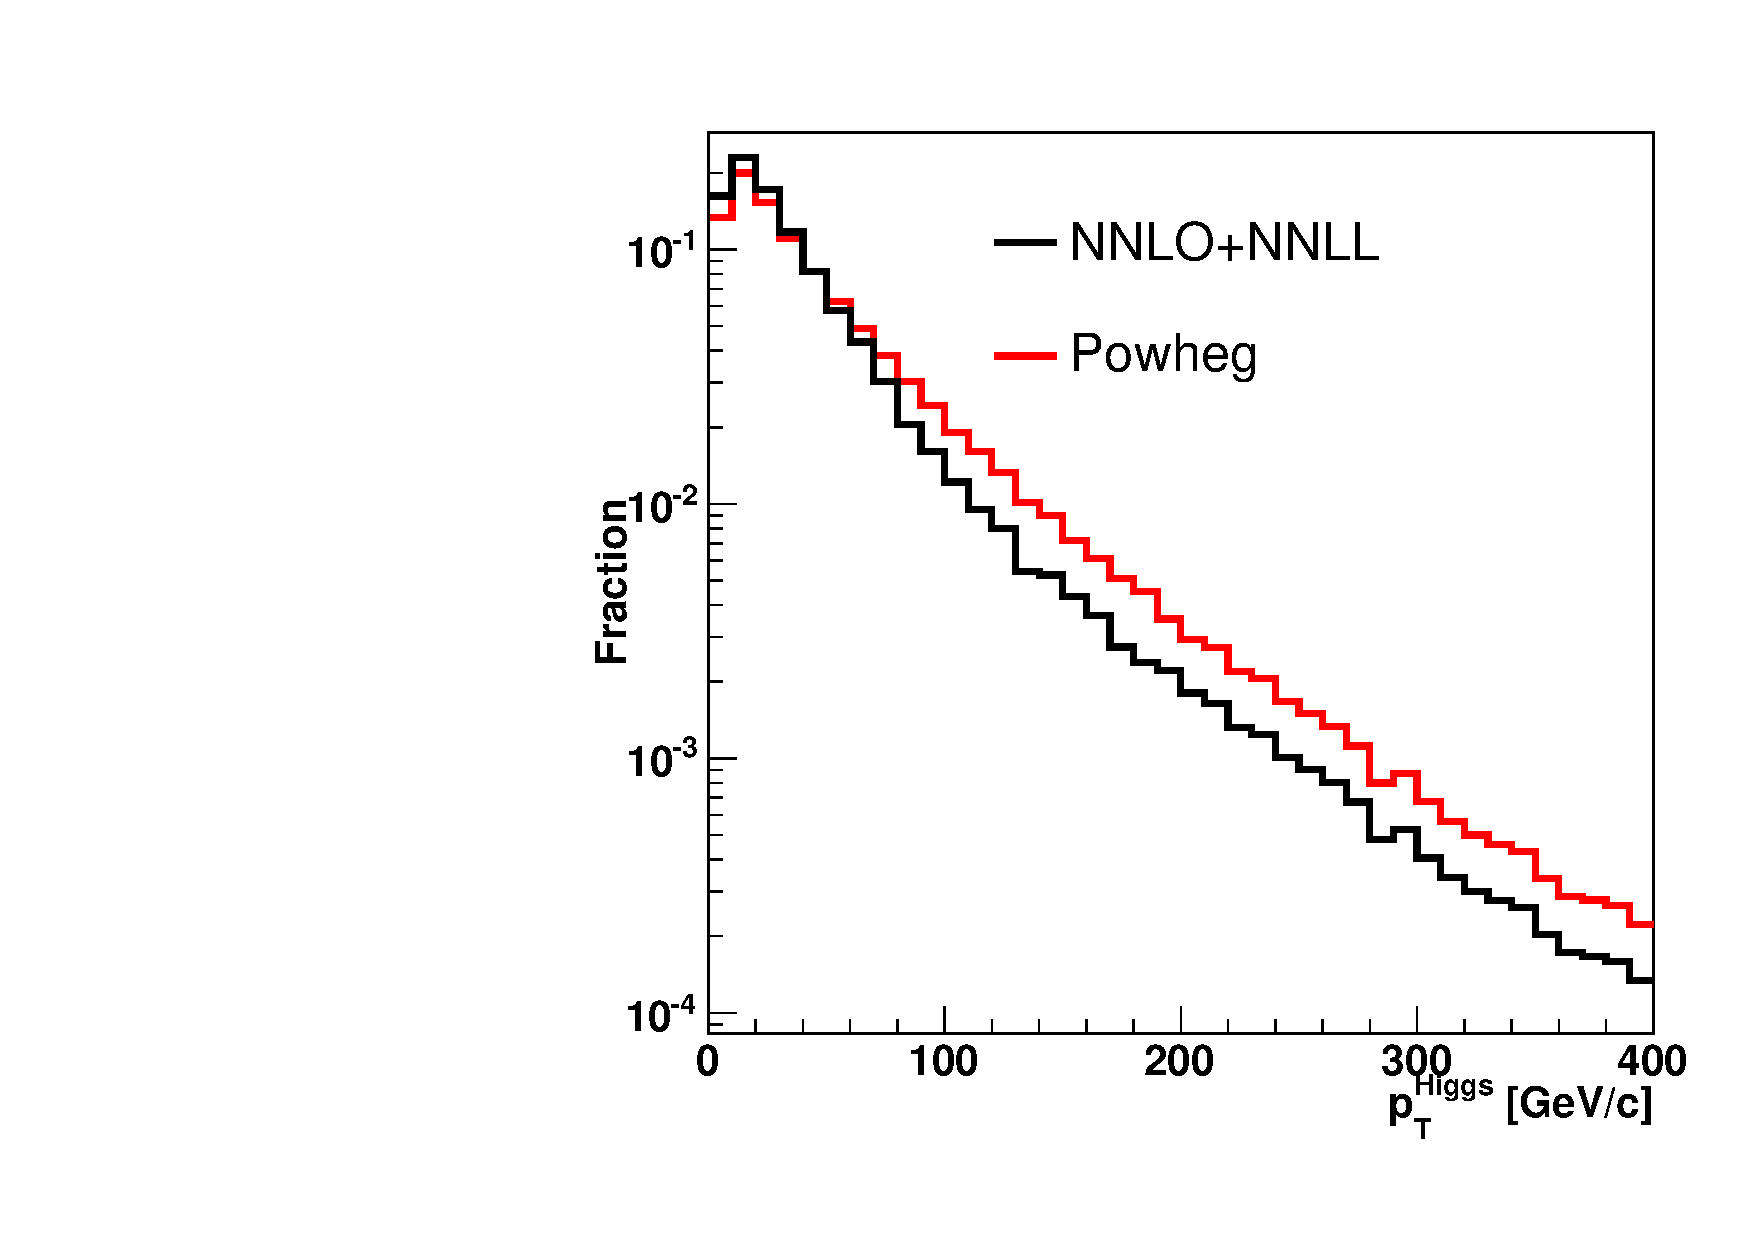
\includegraphics[width=0.49\textwidth]{figures/h160ww_pthiggs.pdf}}
   \subfigure[]{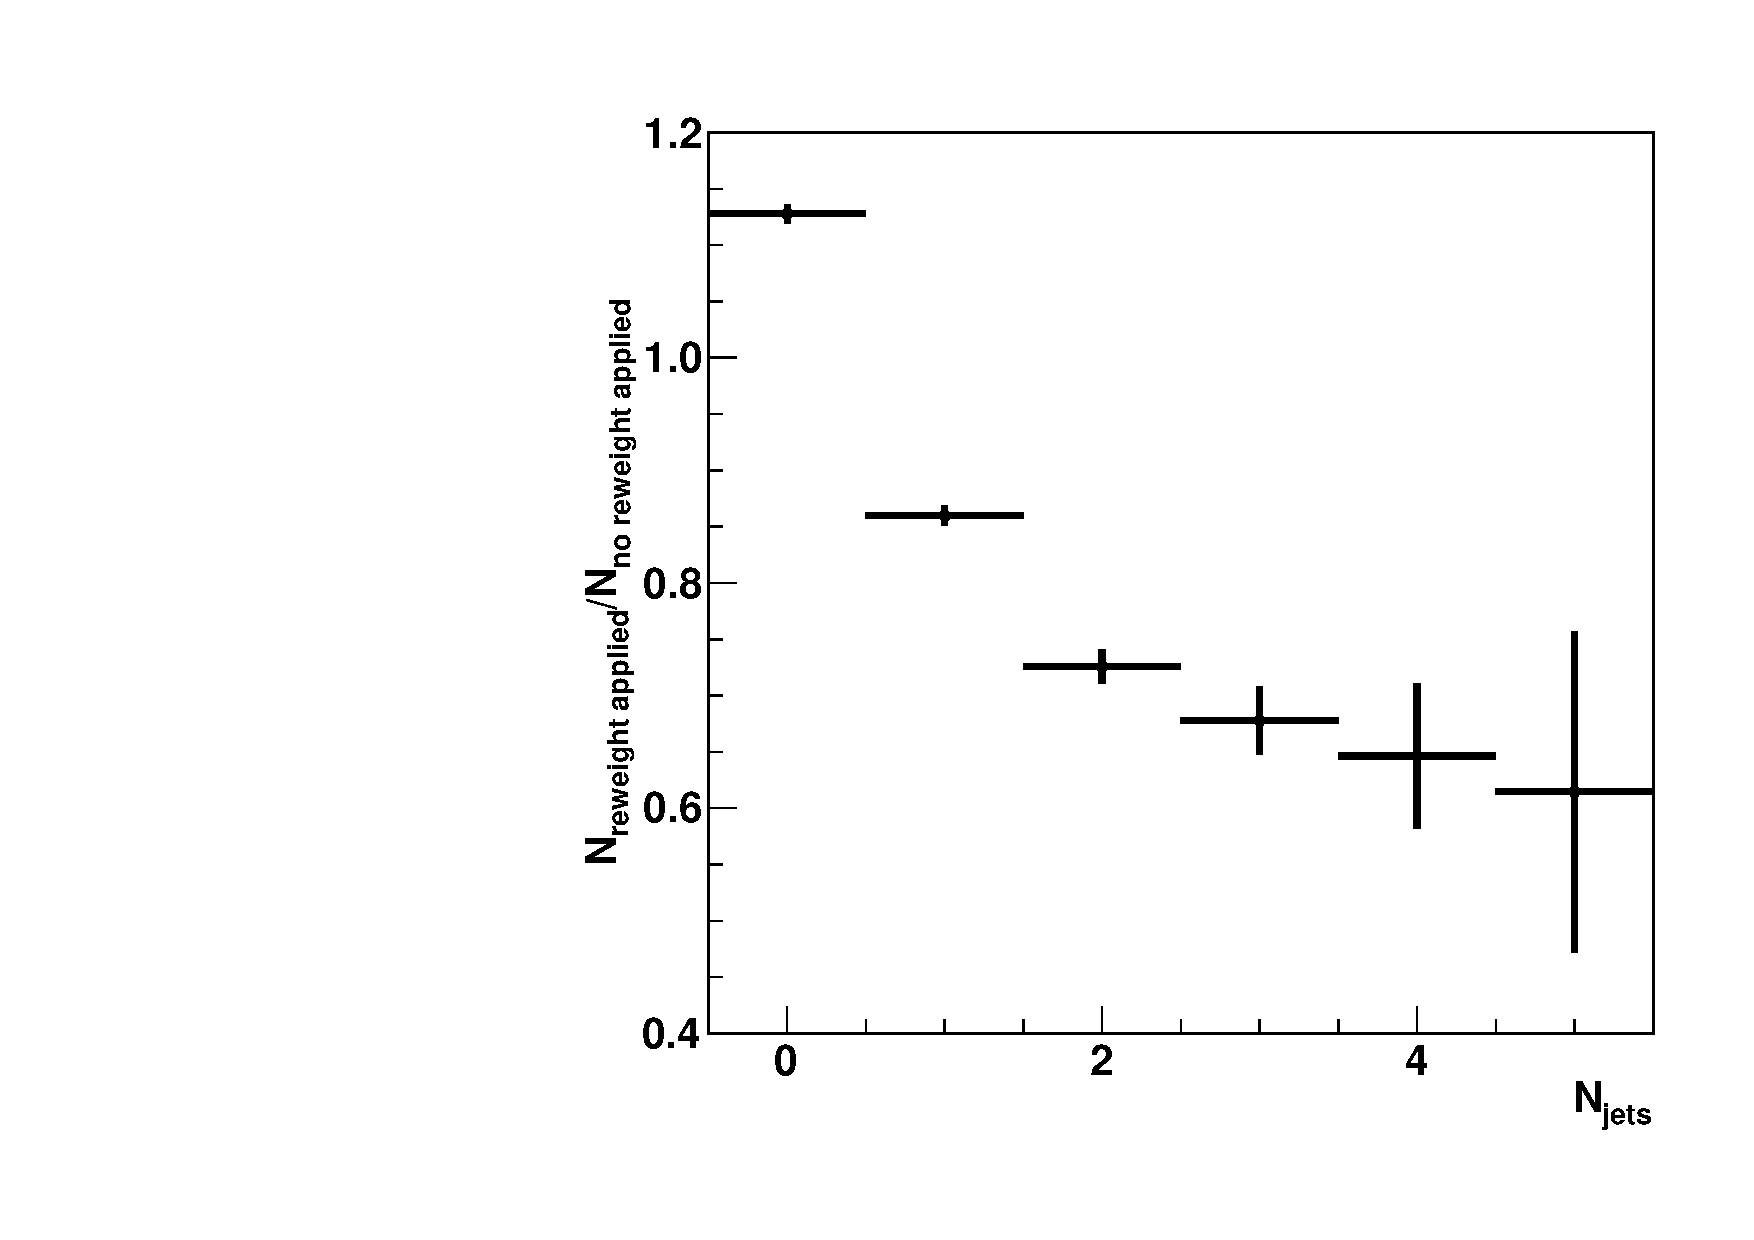
\includegraphics[width=0.49\textwidth]{figures/h160ww_njets_kfactor_ratio.pdf}} 
\caption{(a) Higgs transverse momentum spectrum as predicted by Powheg and the NNLO+NNLL calculation; (b) 
scale factors applied to each jet bin in the Powheg simulation.}
\label{fig:h160ww_pthiggs}
\end{center}
\end{figure}

\end{document}
